% Options for packages loaded elsewhere
\PassOptionsToPackage{unicode}{hyperref}
\PassOptionsToPackage{hyphens}{url}
\PassOptionsToPackage{dvipsnames,svgnames,x11names}{xcolor}
%
\documentclass[
  letterpaper,
  DIV=11,
  numbers=noendperiod]{scrreprt}

\usepackage{amsmath,amssymb}
\usepackage{iftex}
\ifPDFTeX
  \usepackage[T1]{fontenc}
  \usepackage[utf8]{inputenc}
  \usepackage{textcomp} % provide euro and other symbols
\else % if luatex or xetex
  \usepackage{unicode-math}
  \defaultfontfeatures{Scale=MatchLowercase}
  \defaultfontfeatures[\rmfamily]{Ligatures=TeX,Scale=1}
\fi
\usepackage{lmodern}
\ifPDFTeX\else  
    % xetex/luatex font selection
\fi
% Use upquote if available, for straight quotes in verbatim environments
\IfFileExists{upquote.sty}{\usepackage{upquote}}{}
\IfFileExists{microtype.sty}{% use microtype if available
  \usepackage[]{microtype}
  \UseMicrotypeSet[protrusion]{basicmath} % disable protrusion for tt fonts
}{}
\makeatletter
\@ifundefined{KOMAClassName}{% if non-KOMA class
  \IfFileExists{parskip.sty}{%
    \usepackage{parskip}
  }{% else
    \setlength{\parindent}{0pt}
    \setlength{\parskip}{6pt plus 2pt minus 1pt}}
}{% if KOMA class
  \KOMAoptions{parskip=half}}
\makeatother
\usepackage{xcolor}
\setlength{\emergencystretch}{3em} % prevent overfull lines
\setcounter{secnumdepth}{5}
% Make \paragraph and \subparagraph free-standing
\makeatletter
\ifx\paragraph\undefined\else
  \let\oldparagraph\paragraph
  \renewcommand{\paragraph}{
    \@ifstar
      \xxxParagraphStar
      \xxxParagraphNoStar
  }
  \newcommand{\xxxParagraphStar}[1]{\oldparagraph*{#1}\mbox{}}
  \newcommand{\xxxParagraphNoStar}[1]{\oldparagraph{#1}\mbox{}}
\fi
\ifx\subparagraph\undefined\else
  \let\oldsubparagraph\subparagraph
  \renewcommand{\subparagraph}{
    \@ifstar
      \xxxSubParagraphStar
      \xxxSubParagraphNoStar
  }
  \newcommand{\xxxSubParagraphStar}[1]{\oldsubparagraph*{#1}\mbox{}}
  \newcommand{\xxxSubParagraphNoStar}[1]{\oldsubparagraph{#1}\mbox{}}
\fi
\makeatother

\usepackage{color}
\usepackage{fancyvrb}
\newcommand{\VerbBar}{|}
\newcommand{\VERB}{\Verb[commandchars=\\\{\}]}
\DefineVerbatimEnvironment{Highlighting}{Verbatim}{commandchars=\\\{\}}
% Add ',fontsize=\small' for more characters per line
\usepackage{framed}
\definecolor{shadecolor}{RGB}{241,243,245}
\newenvironment{Shaded}{\begin{snugshade}}{\end{snugshade}}
\newcommand{\AlertTok}[1]{\textcolor[rgb]{0.68,0.00,0.00}{#1}}
\newcommand{\AnnotationTok}[1]{\textcolor[rgb]{0.37,0.37,0.37}{#1}}
\newcommand{\AttributeTok}[1]{\textcolor[rgb]{0.40,0.45,0.13}{#1}}
\newcommand{\BaseNTok}[1]{\textcolor[rgb]{0.68,0.00,0.00}{#1}}
\newcommand{\BuiltInTok}[1]{\textcolor[rgb]{0.00,0.23,0.31}{#1}}
\newcommand{\CharTok}[1]{\textcolor[rgb]{0.13,0.47,0.30}{#1}}
\newcommand{\CommentTok}[1]{\textcolor[rgb]{0.37,0.37,0.37}{#1}}
\newcommand{\CommentVarTok}[1]{\textcolor[rgb]{0.37,0.37,0.37}{\textit{#1}}}
\newcommand{\ConstantTok}[1]{\textcolor[rgb]{0.56,0.35,0.01}{#1}}
\newcommand{\ControlFlowTok}[1]{\textcolor[rgb]{0.00,0.23,0.31}{\textbf{#1}}}
\newcommand{\DataTypeTok}[1]{\textcolor[rgb]{0.68,0.00,0.00}{#1}}
\newcommand{\DecValTok}[1]{\textcolor[rgb]{0.68,0.00,0.00}{#1}}
\newcommand{\DocumentationTok}[1]{\textcolor[rgb]{0.37,0.37,0.37}{\textit{#1}}}
\newcommand{\ErrorTok}[1]{\textcolor[rgb]{0.68,0.00,0.00}{#1}}
\newcommand{\ExtensionTok}[1]{\textcolor[rgb]{0.00,0.23,0.31}{#1}}
\newcommand{\FloatTok}[1]{\textcolor[rgb]{0.68,0.00,0.00}{#1}}
\newcommand{\FunctionTok}[1]{\textcolor[rgb]{0.28,0.35,0.67}{#1}}
\newcommand{\ImportTok}[1]{\textcolor[rgb]{0.00,0.46,0.62}{#1}}
\newcommand{\InformationTok}[1]{\textcolor[rgb]{0.37,0.37,0.37}{#1}}
\newcommand{\KeywordTok}[1]{\textcolor[rgb]{0.00,0.23,0.31}{\textbf{#1}}}
\newcommand{\NormalTok}[1]{\textcolor[rgb]{0.00,0.23,0.31}{#1}}
\newcommand{\OperatorTok}[1]{\textcolor[rgb]{0.37,0.37,0.37}{#1}}
\newcommand{\OtherTok}[1]{\textcolor[rgb]{0.00,0.23,0.31}{#1}}
\newcommand{\PreprocessorTok}[1]{\textcolor[rgb]{0.68,0.00,0.00}{#1}}
\newcommand{\RegionMarkerTok}[1]{\textcolor[rgb]{0.00,0.23,0.31}{#1}}
\newcommand{\SpecialCharTok}[1]{\textcolor[rgb]{0.37,0.37,0.37}{#1}}
\newcommand{\SpecialStringTok}[1]{\textcolor[rgb]{0.13,0.47,0.30}{#1}}
\newcommand{\StringTok}[1]{\textcolor[rgb]{0.13,0.47,0.30}{#1}}
\newcommand{\VariableTok}[1]{\textcolor[rgb]{0.07,0.07,0.07}{#1}}
\newcommand{\VerbatimStringTok}[1]{\textcolor[rgb]{0.13,0.47,0.30}{#1}}
\newcommand{\WarningTok}[1]{\textcolor[rgb]{0.37,0.37,0.37}{\textit{#1}}}

\providecommand{\tightlist}{%
  \setlength{\itemsep}{0pt}\setlength{\parskip}{0pt}}\usepackage{longtable,booktabs,array}
\usepackage{calc} % for calculating minipage widths
% Correct order of tables after \paragraph or \subparagraph
\usepackage{etoolbox}
\makeatletter
\patchcmd\longtable{\par}{\if@noskipsec\mbox{}\fi\par}{}{}
\makeatother
% Allow footnotes in longtable head/foot
\IfFileExists{footnotehyper.sty}{\usepackage{footnotehyper}}{\usepackage{footnote}}
\makesavenoteenv{longtable}
\usepackage{graphicx}
\makeatletter
\def\maxwidth{\ifdim\Gin@nat@width>\linewidth\linewidth\else\Gin@nat@width\fi}
\def\maxheight{\ifdim\Gin@nat@height>\textheight\textheight\else\Gin@nat@height\fi}
\makeatother
% Scale images if necessary, so that they will not overflow the page
% margins by default, and it is still possible to overwrite the defaults
% using explicit options in \includegraphics[width, height, ...]{}
\setkeys{Gin}{width=\maxwidth,height=\maxheight,keepaspectratio}
% Set default figure placement to htbp
\makeatletter
\def\fps@figure{htbp}
\makeatother

\KOMAoption{captions}{tableheading}
\makeatletter
\@ifpackageloaded{tcolorbox}{}{\usepackage[skins,breakable]{tcolorbox}}
\@ifpackageloaded{fontawesome5}{}{\usepackage{fontawesome5}}
\definecolor{quarto-callout-color}{HTML}{909090}
\definecolor{quarto-callout-note-color}{HTML}{0758E5}
\definecolor{quarto-callout-important-color}{HTML}{CC1914}
\definecolor{quarto-callout-warning-color}{HTML}{EB9113}
\definecolor{quarto-callout-tip-color}{HTML}{00A047}
\definecolor{quarto-callout-caution-color}{HTML}{FC5300}
\definecolor{quarto-callout-color-frame}{HTML}{acacac}
\definecolor{quarto-callout-note-color-frame}{HTML}{4582ec}
\definecolor{quarto-callout-important-color-frame}{HTML}{d9534f}
\definecolor{quarto-callout-warning-color-frame}{HTML}{f0ad4e}
\definecolor{quarto-callout-tip-color-frame}{HTML}{02b875}
\definecolor{quarto-callout-caution-color-frame}{HTML}{fd7e14}
\makeatother
\makeatletter
\@ifpackageloaded{caption}{}{\usepackage{caption}}
\AtBeginDocument{%
\ifdefined\contentsname
  \renewcommand*\contentsname{Table of contents}
\else
  \newcommand\contentsname{Table of contents}
\fi
\ifdefined\listfigurename
  \renewcommand*\listfigurename{List of Figures}
\else
  \newcommand\listfigurename{List of Figures}
\fi
\ifdefined\listtablename
  \renewcommand*\listtablename{List of Tables}
\else
  \newcommand\listtablename{List of Tables}
\fi
\ifdefined\figurename
  \renewcommand*\figurename{Figure}
\else
  \newcommand\figurename{Figure}
\fi
\ifdefined\tablename
  \renewcommand*\tablename{Table}
\else
  \newcommand\tablename{Table}
\fi
}
\@ifpackageloaded{float}{}{\usepackage{float}}
\floatstyle{ruled}
\@ifundefined{c@chapter}{\newfloat{codelisting}{h}{lop}}{\newfloat{codelisting}{h}{lop}[chapter]}
\floatname{codelisting}{Listing}
\newcommand*\listoflistings{\listof{codelisting}{List of Listings}}
\makeatother
\makeatletter
\makeatother
\makeatletter
\@ifpackageloaded{caption}{}{\usepackage{caption}}
\@ifpackageloaded{subcaption}{}{\usepackage{subcaption}}
\makeatother

\ifLuaTeX
  \usepackage{selnolig}  % disable illegal ligatures
\fi
\usepackage{bookmark}

\IfFileExists{xurl.sty}{\usepackage{xurl}}{} % add URL line breaks if available
\urlstyle{same} % disable monospaced font for URLs
\hypersetup{
  pdftitle={Data Science at SAMY},
  colorlinks=true,
  linkcolor={blue},
  filecolor={Maroon},
  citecolor={Blue},
  urlcolor={Blue},
  pdfcreator={LaTeX via pandoc}}


\title{Data Science at SAMY}
\author{}
\date{}

\begin{document}
\maketitle

\renewcommand*\contentsname{Table of contents}
{
\hypersetup{linkcolor=}
\setcounter{tocdepth}{2}
\tableofcontents
}

\chapter{Welcome to the Data Science
Handbook}\label{welcome-to-the-data-science-handbook}

Welcome to our Data Science Handbook, your comprehensive guide to the
methods, case studies, and best practices that define our approach to
data science here at SAMY. This handbook is designed to be a dynamic
resource for our team, evolving with new insights, tools, and
technologies.

Within these pages, you'll find detailed case studies showcasing our
successful projects, high-level concepts that underpin our strategies,
and practical coding examples to help you apply these techniques in your
own work. Irrespective of your experience in data science, this handbook
aims to provide valuable insights and practical guidance to enhance your
skills and knowledge.

We believe that sharing knowledge and continuously learning are key to
staying ahead in the fast-paced world of data science. As such, this
handbook is not just a static document but a collaborative space where
ideas are exchanged, and innovation thrives.

Happy data sciencing!

\begin{tcolorbox}[enhanced jigsaw, colback=white, opacitybacktitle=0.6, coltitle=black, left=2mm, breakable, bottomtitle=1mm, toptitle=1mm, toprule=.15mm, colframe=quarto-callout-note-color-frame, titlerule=0mm, title=\textcolor{quarto-callout-note-color}{\faInfo}\hspace{0.5em}{Note}, colbacktitle=quarto-callout-note-color!10!white, rightrule=.15mm, bottomrule=.15mm, arc=.35mm, opacityback=0, leftrule=.75mm]

If you have any questions at all, ask any member of the team. Whilst
this Handbook aims to be a valuable resource for self-learning, it can
often be more beneficial to spend 5 minutes talking through a concept
with someone on the team who may be able to describe something in a
different manner to this document.

\end{tcolorbox}

\part{Introduction}

\chapter{The Data Science team}\label{the-data-science-team}

\section{Where we sit}\label{where-we-sit}

\begin{quote}
The Data Science department are a fully global resource within the
alliance
\end{quote}

Capture Intelligence is our biggest internal ``client'' as there are
plenty of opportunities to offer data science led services in the
research offering of Capture. But also have our own core central pipe
for development that supports \emph{all} agency brands.

What this means is as a team we have responsibilities that range from
continual development of our own tech stack to help answer specific
research questions for external clients to helping empower members of
the alliance to use mindful applications of emerging technologies.

\section{Who we are}\label{who-we-are}

\textbf{Mike Tapp}: Data Director

\textbf{Jack Penzer}: Global Data Product Lead

\textbf{Jamie Hudson}: Senior Data Scientist

\textbf{Aoife Ryan}: Data Scientist

\textbf{Sophie Thomas}: Jr.~Data Scientist

\part{Case Studies}

\chapter{Peaks and Pits}\label{peaks-and-pits}

``Peaks and Pits'' is one of our fundamental project offerings and a
workflow that is a solid representation of good data science work that
we perform.

\section{What is the concept/project
background?}\label{what-is-the-conceptproject-background}

Strong memories associated to brands or products go deeper than simple
positive or negative sentiment. Most of our experiences are not encoded
in memory, rather what we remember about experiences are changes,
significant moments, and endings. In their book ``The Power of
Moments'', two psychologists
(\href{https://heathbrothers.com/about/}{Chip and Dan Heath}) define
these core memories as Peak and Pits, impactful experiences in our
lives.

Broadly, peak moments are experiences that stand our memorable in our
lives in a positive sense, whereas pit moments are impactful negative
experiences.

Microsoft tasked us with finding a way to identify these moments in
social data- going beyond `simple' positive and negative sentiment which
does not tell the full story of consumer/user experience. The end goal
is that by providing Microsoft with these peak and pit moments in the
customer experience, they can design peak moments in addition to simply
removing pit moments.

\subsection{The end goal}\label{the-end-goal}

With these projects the core final `product' is a collection of
different peaks and pits, with suitable representative verbatims and an
explanation to understand the high-level intricacies of these different
emotional moments.

\begin{figure}[H]

{\centering \includegraphics{img/peaks_list.png}

}

\caption{Screenshot from a Peaks and Pits project showcasing the
identified Peak moments for a product at a high level}

\end{figure}%

\subsection{Key features of project}\label{key-features-of-project}

\begin{itemize}
\tightlist
\item
  There is no out-of-the-box ML model available whose purpose is to
  classify social media posts as either peaks or pits (i.e.~we cannot
  use a ready-made solution, we must design our own bespoke solution).
\item
  There is limited data available

  \begin{itemize}
  \tightlist
  \item
    Unlike the case of spam/ham or sentiment classification, there is
    not a bank of pre-labelled data available for us to leverage for
    `traditional ML'.
  \end{itemize}
\item
  Despite these issues, the research problem itself is well defined
  (\textbf{what} are the core peak and pit moments for a brand/product),
  and because there are only three classes (peak, pit, or neither) which
  are based on extensive research, the classes themselves are well
  described (even if it is case of ``you know a peak moment when you see
  it'').
\end{itemize}

\section{Overview of approach}\label{overview-of-approach}

Peaks and pits projects have gone through many iterations throughout the
past year and a half. Currently, the general workflow is to use utilise
a model framework known as
\href{https://huggingface.co/docs/setfit/conceptual_guides/setfit}{SetFit}
to efficiently train a text classification model with limited training
data. This fine-tuned model is then able to run inference over large
datasets to label posts as either peaks, pits, or neither. We then
utilise the LLM capabilities to refine these peak and pit moments into a
collection of posts we are extremely confident are peaks and/or pits. We
then employ topic modelling to identify groups of similar peaks and pits
to help us organise and discover hidden topics or themes within this
collection of core moments.

This whole process can be split into six distinct steps:

\begin{enumerate}
\def\labelenumi{\arabic{enumi}.}
\tightlist
\item
  \hyperref[step-one]{Extract brand/product mentions from Sprinklr (the
  start of any project)}
\item
  \hyperref[step-two]{Obtain project-specific exemplar posts to help
  fine-tune a text classification model}
\item
  \hyperref[step-three]{Perform model fine-tuning through contrastive
  learning}
\item
  \hyperref[step-four]{Run inference over all of the project specific
  data}
\item
  \hyperref[step-five]{Use GPT-3.5 for an extra layer of classification
  on identified peaks and pits}
\item
  \hyperref[step-six]{Turn moments into something interpretable using
  topic modelling}
\end{enumerate}

\begin{figure}[H]

{\centering \includegraphics[width=0.8\textwidth,height=\textheight]{./img/ar_workflow.png}

}

\caption{Schematic workflow from Project 706 - Peaks and Pits in M365
Apps}

\end{figure}%

\subsection{Obtain posts for the project (Step 1)}\label{step-one}

This step relies on the analysts to export relevant mentions from
Sprinklr (one of the social listening tools that analysts utilise to
obtain social data), and therefore is not detailed much here. What is
required is one dataset for each of the brands/products, so they can be
analysed separately.

\subsection{Identify project-specific exemplar peaks and pits to
fine-tune our ML model (Step 2)}\label{step-two}

This step is synonymous with data labelling required for any machine
learning project where annotated data is not already available.

Whilst there is no one-size-fits-all for determining the amount of data
required to train a machine learning model, for traditional models and
tasks, the number of examples per label is often in the region of
thousands, and often this isn't even enough for more complex problems.

The time required to accurately label thousands of peaks and pits to
train a classification model in the traditional way is sadly beyond the
scope of feasibility for our projects. As such we needed an approach
that did not rely on copious amounts of pre-labelled data.

This is where
\href{https://huggingface.co/docs/setfit/conceptual_guides/setfit}{SetFit}
comes in. As mentioned previously, SetFit is a framework that enables us
to efficiently train a text classification model with limited training
data.

\begin{tcolorbox}[enhanced jigsaw, colback=white, opacitybacktitle=0.6, coltitle=black, left=2mm, breakable, bottomtitle=1mm, toptitle=1mm, toprule=.15mm, colframe=quarto-callout-tip-color-frame, titlerule=0mm, title=\textcolor{quarto-callout-tip-color}{\faLightbulb}\hspace{0.5em}{How does it do this?}, colbacktitle=quarto-callout-tip-color!10!white, rightrule=.15mm, bottomrule=.15mm, arc=.35mm, opacityback=0, leftrule=.75mm]

\emph{Note the below is directly copied from the SetFit documentation.
It is so succinctly written that trying to rewrite it would not do it
justice.}

Every SetFit model consists of two parts: a \textbf{sentence
transformer} embedding model (the body) and a \textbf{classifier} (the
head). These two parts are trained in two separate phases: the
\textbf{embedding finetuning phase} and the \textbf{classifier training
phase}. This conceptual guide will elaborate on the intuition between
these phases, and why SetFit works so well.

\textbf{Embedding finetuning phase}

The first phase has one primary goal: finetune a sentence transformer
embedding model to produce useful embeddings for our classification
task. The Hugging Face Hub already has thousands of sentence transformer
available, many of which have been trained to very accurately group the
embeddings of texts with similar semantic meaning.

However, models that are good at Semantic Textual Similarity (STS) are
not necessarily immediately good at our classification task. For
example, according to an embedding model, the sentence of 1)
``\texttt{He\ biked\ to\ work.}'' will be much more similar to 2)
``\texttt{He\ drove\ his\ car\ to\ work.}'' than to 3)
``\texttt{Peter\ decided\ to\ take\ the\ bicycle\ to\ the\ beach\ party!}''.
But if our classification task involves classifying texts into
transportation modes, then we want our embedding model to place
sentences 1 and 3 closely together, and 2 further away.

To do so, we can finetune the chosen sentence transformer embedding
model. The goal here is to nudge the model to use its pretrained
knowledge in a different way that better aligns with our classification
task, rather than making the completely forget what it has learned.

For finetuning, SetFit uses \textbf{contrastive learning}. This training
approach involves creating \textbf{positive and negative pairs} of
sentences. A sentence pair will be positive if both of the sentences are
of the same class, and negative otherwise. For example, in the case of
binary ``positive''-``negative'' sentiment analysis,
(``\texttt{The\ movie\ was\ awesome}'', ``\texttt{I\ loved\ it}'') is a
positive pair, and (``\texttt{The\ movie\ was\ awesome}'',
``\texttt{It\ was\ quite\ disappointing}'') is a negative pair.

During training, the embedding model receives these pairs, and will
convert the sentences to embeddings. If the pair is positive, then it
will pull on the model weights such that the text embeddings will be
more similar, and vice versa for a negative pair. Through this approach,
sentences with the same label will be embedded more similarly, and
sentences with different labels less similarly.

Conveniently, this contrastive learning works with pairs rather than
individual samples, and we can create plenty of unique pairs from just a
few samples. For example, given 8 positive sentences and 8 negative
sentences, we can create 28 positive pairs and 64 negative pairs for 92
unique training pairs. This grows exponentially to the number of
sentences and classes, and that is why SetFit can train with just a few
examples and still correctly finetune the sentence transformer embedding
model. However, we should still be wary of overfitting.

\textbf{Classifier training phase}

Once the sentence transformer embedding model has been finetuned for our
task at hand, we can start training the classifier. This phase has one
primary goal: create a good mapping from the sentence transformer
embeddings to the classes.

Unlike with the first phase, training the classifier is done from
scratch and using the labelled samples directly, rather than using
pairs. By default, the classifier is a simple \textbf{logistic
regression} classifier from scikit-learn. First, all training sentences
are fed through the now-finetuned sentence transformer embedding model,
and then the sentence embeddings and labels are used to fit the logistic
regression classifier. The result is a strong and efficient classifier.

Using these two parts, SetFit models are efficient, performant and easy
to train, even on CPU-only devices.

\end{tcolorbox}

There is no perfect number of labelled examples to find per class
(i.e.~peak, pit, or neither). Whilst in general more exemplars (and
hence more training data) is beneficial, having fewer but high quality
labelled posts is far superior than more posts of poorer quality. This
is extremely important due to the contrastive nature of SetFit where
it's superpower is making the most of few, extremely good, labelled
data.

Okay so now we know why we need labelled data, and we know what the
model will do with it, \emph{what is our approach} for obtaining the
labelled data?

Broadly, we use our human judgement to read a post from the current
project dataset, and manually label whether we think it is a peak, a
pit, or neither. To avoid us just blindly reading through random posts
in the dataset in the hope of finding good examples (this is not a good
use of time), we can employ a couple of tricks to narrow our search
region to posts that have a reasonable likelihood of being suitable
examples.

\begin{enumerate}
\def\labelenumi{\arabic{enumi})}
\item
  The first trick is to use the OpenAI API to access a GPT model. This
  involves taking a sample of posts (say \textasciitilde1000) and
  running these through a GPT model, with a prompt that asks the model
  to classify each post into either a peak, pit, or neither. This is
  possible because GPT models have learned knowledge of peaks and pits
  from its training on large datasets. We can therefore get a human to
  only sense-check/label posts that GPT also believes are peaks or pits.
\item
  The second trick involves using a previously created SetFit model
  (i.e.~from an older project), and running inference over a similar
  sample of posts (again, say \textasciitilde1000).
\end{enumerate}

We would tend to suggest the OpenAI route, as it is simpler to implement
(in our opinion), and often the old SetFit model has been finetuned on
data from a different domain so it might struggle to understand domain
specific language in the current dataset. However, be aware if it not as
scalable as using an old SetFit model and has the drawback of being a
prompt based classification of a black-box model (as well as issues
relating to cost and API stability).

Irrespective of which approach is taken, by the end of this step we need
to have a list of example posts we are confident represent what a peak
or pit moment looks like for each particular product we are researching,
including posts that are ``neither''.

\begin{tcolorbox}[enhanced jigsaw, colback=white, opacitybacktitle=0.6, coltitle=black, left=2mm, breakable, bottomtitle=1mm, toptitle=1mm, toprule=.15mm, colframe=quarto-callout-note-color-frame, titlerule=0mm, title=\textcolor{quarto-callout-note-color}{\faInfo}\hspace{0.5em}{Why do we do this for each project?}, colbacktitle=quarto-callout-note-color!10!white, rightrule=.15mm, bottomrule=.15mm, arc=.35mm, opacityback=0, leftrule=.75mm]

After so many projects now don't we already have a good idea of what a
peak and pit moment for the purposes of model training?

Each peak and pit project we work on has the potential to introduce
`domain' specific language, which a machine learning classifier (model)
may not have seen before. By manually identifying exemplar peaks and
pits that are project-specific, this gives our model the best chance to
identify emotional moments appropriate to the project/data at hand.

The obvious case for this is with gaming specific language, where terms
that don't necessarily relate to an `obvious' peak or pit moment could
refer to one the gaming conversation, for example the terms/phrases
``GG'', ``camping'', ``scrub'', and ``goat'' all have very specific
meanings in this domain that differ from their use in everyday language.

\end{tcolorbox}

\subsection{Train our model using our labelled examples (Step
3)}\label{step-three}

Before we begin training our SetFit model with our data, it's necessary
to clean and wrangle the fine-tuning datasets. Specifically, we need to
mask any mentions of brands or products to prevent bias. For instance,
if a certain brand frequently appears in the training data within peak
contexts, the model could erroneously link peak moments to that brand
rather than learning the peak-language expressed in the text.

\begin{quote}
This precaution should extend to all aspects of our training data that
might introduce biases. For example, as we now have examples from
various projects, an overrepresentation of data from `gaming projects'
in our `peak' posts within our training set (as opposed to the `pit'
posts) could skew the model into associating gaming-related language
more with peaks than pits.
\end{quote}

Broadly the cleaning steps that should be applied to our data for
finetuning are:

\begin{itemize}
\tightlist
\item
  Mask brand/product mentions
\item
  Remove hashtags \#️⃣
\item
  Remove mentions 💬
\item
  Remove URLs 🌐
\item
  Remove emojis 🐙
\end{itemize}

\begin{tcolorbox}[enhanced jigsaw, colback=white, opacitybacktitle=0.6, coltitle=black, left=2mm, breakable, bottomtitle=1mm, toptitle=1mm, toprule=.15mm, colframe=quarto-callout-note-color-frame, titlerule=0mm, title=\textcolor{quarto-callout-note-color}{\faInfo}\hspace{0.5em}{What about other cleaning steps?}, colbacktitle=quarto-callout-note-color!10!white, rightrule=.15mm, bottomrule=.15mm, arc=.35mm, opacityback=0, leftrule=.75mm]

You will notice here we do not remove stop words-. As explained in the
previous step, part of the finetuning process is to finetune a sentence
embedding model, and we want to keep stop words so that we can use the
full context of the post in order to finetune accurate embeddings.

\end{tcolorbox}

At this step, we can split out our data into training, testing, and
validation datasets. A good rule of thumb is to split the data 70\% to
training data, 15\% to testing data, and 15\% to validation data. By
default,
\href{https://huggingface.co/docs/setfit/v1.0.3/en/conceptual_guides/sampling_strategies}{SetFit
oversamples} the minimum class within the training data, so we
\emph{shouldn't} have to worry too much about imbalanced datasets-
though be aware if we have extreme imbalanced we will end up sampling
the same contrastive pairs (normally positive pairs) multiple times.
However, our experimentation has shown that class imbalance doesn't seem
to have a significant effect to the training/output of the SetFit model
for peaks and pits.

We are now at the stage where we can actually fine-tune the model. There
are many different parameters we can change when fine-tuning the model,
such as the specific embedding model used, the number of epochs to train
for, the number of contrastive pairs of sentences to train on etc. For
more details, please refer to the
\href{https://jamiehshare.github.io/peaks-pits-bookdown/step-four.html}{Peaks
and Pits Playbook}

We can assess model performance on the testing dataset by looking at
accuracy, precision, recall, and F1 scores. For peaks and pits, the most
important metric is actually \textbf{recall} because in
\hyperref[step-four]{step 4} we reclassify posts using GPT, so we want
to make sure we are able to provide \emph{as many true peak/pit moments
as possible} to this step, even if it means we also provide a few false
positives.

\begin{tcolorbox}[enhanced jigsaw, colback=white, opacitybacktitle=0.6, coltitle=black, left=2mm, breakable, bottomtitle=1mm, toptitle=1mm, toprule=.15mm, colframe=quarto-callout-note-color-frame, titlerule=0mm, title=\textcolor{quarto-callout-note-color}{\faInfo}\hspace{0.5em}{Click here for more info as to why recall is most important}, colbacktitle=quarto-callout-note-color!10!white, rightrule=.15mm, bottomrule=.15mm, arc=.35mm, opacityback=0, leftrule=.75mm]

As a refresher, \texttt{precision} is the \emph{proportion of positive
identifications} that are actually \emph{correct} (it focuses on the
correctness of positive predictions) whereas \texttt{recall} is the
\emph{proportion of actual positives} that are identified correctly (it
focuses on capturing all relevant instances).

In cases where false positives need to be minimised (incorrectly
predicting a non-event as an event) we need to prioritise
\texttt{precision} - if you've built a model to identify hot dogs from
regular ol' doggos, high precision ensures that normal dogs are not
misclassified as hot dogs.

In cases where false negatives need to be minimised (failing to detect
an actual event) we need to prioritise \texttt{recall} - in medical
diagnoses we need to minimise the number of times a patient is
incorrectly told they \emph{do not} have a disease when in reality they
\emph{do} (or worded differently, we need to ensure that
\textbf{\emph{all}} patients with a disease are identified).

To apply this to our problem- we want to be sure that we capture all (or
as many as possible) relevant instances of peaks or pits- even if a few
false positives come in (neither posts that are incorrectly classified
as peaks or pits). As we use GPT to make further peak/pit
identifications, it's better to provide GPT with with a comprehensive
set of potential peaks and pits, including some incorrect ones, than to
miss out on critical data.

\end{tcolorbox}

\subsubsection*{Visualise model
separation}\label{visualise-model-separation}
\addcontentsline{toc}{subsubsection}{Visualise model separation}

As a bonus, we can actually neatly visualise how well our finetuning of
the sentence transformer embedding model has gone- by seeing how well
the model is able to separate our different classes in embedding space.

We can do this by visualising the 2-D structure of the embeddings and
see how they cluster:

This is what it looks the embeddings space looks like on an un-finetuned
model:

\begin{figure}[H]

{\centering \includegraphics{./img/embedding_untrained.png}

}

\caption{Un-finetuned embedding model}

\end{figure}%

Here we can see that posts we know are peaks, pits, and neither all
overlap and there is no real structure in the data. Any clustering of
points observed are probably due to the posts' semantic similarity (c.f.
the mode of transport example above). We would not be able to nicely use
a classifier model to get a good mapping from this embedding space to
our classes (i.e.~we couldn't easily separate classes here).

By visualising the same posts after finetuning the embedding model, we
get something more like this, where we can see that the embedding model
now clearly separates posts based on their peak/pit classification
(though we must be wary of overfitting!).

\begin{figure}[H]

{\centering \includegraphics{./img/embedding_trained.png}

}

\caption{Finetuned embedding model}

\end{figure}%

Finally, now we are happy with our model performance based on the
training and validation datasets, we can evaluate the performance of
this final model using our testing data. This is data that the model has
never seen, and we are hoping that the accuracy and performance is
similar to that of the validation data. This is Machine Learning 101 and
if a refresher is needed for this there are plenty of resources online
looking at the role of training, validation, and testing data.

\subsection{Run inference over project data (Step 4)}\label{step-four}

It is finally time to infer whether the project data contain peaks or
pits by using our fine-tuned SetFit model to classify the posts.

Before doing this again we need to make sure we do some data cleaning on
the project specific data.

Broadly, this needs to match the high-level cleaning we did during
fine-tuning stage:

\begin{itemize}
\tightlist
\item
  Mask brand/product mentions (using RoBERTa-based model {[}or
  similar{]} and \texttt{Rivendell} functions)
\item
  Remove hashtags \#️⃣
\item
  Remove mentions 💬
\item
  Remove URLs 🌐
\item
  Remove emojis 🐙
\end{itemize}

\begin{tcolorbox}[enhanced jigsaw, colback=white, opacitybacktitle=0.6, coltitle=black, left=2mm, breakable, bottomtitle=1mm, toptitle=1mm, toprule=.15mm, colframe=quarto-callout-warning-color-frame, titlerule=0mm, title=\textcolor{quarto-callout-warning-color}{\faExclamationTriangle}\hspace{0.5em}{Note on social media sources}, colbacktitle=quarto-callout-warning-color!10!white, rightrule=.15mm, bottomrule=.15mm, arc=.35mm, opacityback=0, leftrule=.75mm]

Currently all peak and pit projects have been done on Twitter or Reddit
data, but if a project includes web/forum data quirky special
characters, numbered usernames, structured quotes etc. should also be
removed.

\end{tcolorbox}

Okay now we can \emph{finally} run inference. This is extremely simple
and only requires a couple of lines of code (again see the
\href{https://jamiehshare.github.io/peaks-pits-bookdown/step-five.html}{Peaks
and Pits Playbook for code implementation})

\subsection{The metal detector, GPT-3.5 (Step 5)}\label{step-five}

During \hyperref[step-four]{step 4} we obtained peak and pit
classification using few-shot classification with SetFit. The benefit of
this approach (as outlined previously) is its speed and ability to
classify with very few labelled samples due to contrastive learning.

However, during our iterations of peak and pit projects, we've realised
that this step still classifies a fair amount of non-peak and pit posts
incorrectly. This can cause noise in the downstream analyses and be very
time consuming for us to further trudge through verbatims.

As such, the aim of this step is to further our confidence in our final
list of peaks and pits to be \emph{actually} peaks and pits. Remember
before we explained that for SetFit, we focussed on \textbf{recall}
being the most important measure in our business case? This is where we
assume that GPT-3.5 enables us to remove the false positives due to it's
incredibly high performance.

\begin{tcolorbox}[enhanced jigsaw, colback=white, opacitybacktitle=0.6, coltitle=black, left=2mm, breakable, bottomtitle=1mm, toptitle=1mm, toprule=.15mm, colframe=quarto-callout-important-color-frame, titlerule=0mm, title=\textcolor{quarto-callout-important-color}{\faExclamation}\hspace{0.5em}{Why not use GPT from the start?}, colbacktitle=quarto-callout-important-color!10!white, rightrule=.15mm, bottomrule=.15mm, arc=.35mm, opacityback=0, leftrule=.75mm]

Using GPT-3.5 for inference, even over relatively few posts as in peaks
and pits, is expensive both in terms of time and money. Preliminary
tests have suggested it is in the order of magnitude of thousands of
times slower than SetFit. It is for these reasons why we do not use
GPT-x models from the get go, despite it's obvious incredible
understanding of natural language.

\end{tcolorbox}

Whilst prompt-based classification such as those with GPT-3.5 certainly
has its drawbacks (dependency on prompt quality, prompt injections in
posts, handling and version control of complex prompts, unexpected
updates to the model weights rendering prompts ineffective), the
benefits include increased flexibility in what we can ask the model to
do. As such, in the absence of an accurate, cheap, and quick model to
perform span detection, we have found that often posts identified as
peaks/pits did indeed use peak/pit language, but the context of the
moment was not related to the brand/product at the core of the research
project.

For example, take the post that we identified in the project 706,
looking for peaks and pits relating to PowerPoint:

\begin{quote}
This brings me so much happiness! Being a non-binary graduate student in
STEM academia can be challenging at times. Despite using my they/them
pronouns during introductions, emails, powerpoint presentations, name
tags, etc. my identity is continuously mistaken. Community is key!
\end{quote}

This is clearly a `peak', however it is not accurate or valid to
attribute this memorable moment to PowerPoint. Indeed, PowerPoint is
merely mentioned in the post, but is not a core driver of the Peak which
relates to feeling connection and being part of a community. This is as
much a PowerPoint Peak as it is a Peak for the use of emails.

Therefore, we can engineer our prompt to include a caveat to say that
the specific peak or pit moment must relate directly to the
brand/product usage (if relevant).

\subsection{Topic modelling to make sense of our data (Step
6)}\label{step-six}

Now we have an extremely refined set of posts classified as either peak
or pits. The next step is to identify what these moments actually relate
to (i.e.~identify the topics of these moments through statistical
methods).

To do this, we employ topic modelling via
\href{https://maartengr.github.io/BERTopic/index.html}{BERTopic} to
identifying high-level topics that emerge within the peak and pit
conversation. This is done separately for each product and peak/pit
dataset (i.e.~there will be one BERTopic model for product A peaks,
another BERTopic model for product A pits, an additional BERTopic model
for product B peaks etc).

We implement BERTopic using the R package BertopicR. As there is already
\href{https://aoiferyan-sc.github.io/BertopicR/}{good documentation on
BertopicR} this section will not go into any technical detail in regards
to implementation.

From BertopicR. we end up with a topic label for each post in our
dataset, meaning we can easily quantify the size of each topics and
visualise temporal patterns of topic volume etc.

\chapter{Conversation Landscape}\label{conversation-landscape}

The `Conversation Landscape' method has proven to be an effective tool
for querying, auditing, and analysing both broad concepts and finely
grained topics across social conversations on all major platforms, as
well as web pages and forums.

\section{Project Background}\label{project-background}

Working with semi-structured or unstructured high-dimensional data, such
as text (and in our case, social media posts), poses significant
challenges in measuring or quantifying the language used to describe any
specific phenomena. One common approach to quantifying language is topic
modelling, where a corpus (or collection of documents) is processed and
later represented in neater and simplified format. This often involves
displaying top terms, verbatims, or threads highlighting any nuances or
differences within the data. Traditional topic modelling or text
analysis methods, such as Latent Dirichlet Allocation (LDA), operate on
the probability or likelihood of terms or n-grams belonging to a set
number of topics.

The Conversation Landscape workflow offers a slightly different solution
and one that partitions text data without a specific need for burdening
the user with sifting through rows of data in order to segment documents
with hopes of understanding or recognising any differences in language,
which would ideally be defined more simply as topics. The is mostly
achieved through sentence transforming, where documents are converted
from words to numerical values, which are often referred to as
`embeddings'. These values are calculated based on their content's
semantic and syntactic properties. The transformed values are then
processed again using dimension reduction techniques, making the data
more suitable for visualisation. Typically, this involves reducing to
two dimensions, though three dimensions may be used to introduce another
layer of abstraction between our data points. The example provided
throughout this chapter, represents some text data as nodes upon a
two-dimensional space.

\begin{tcolorbox}[enhanced jigsaw, colback=white, opacitybacktitle=0.6, coltitle=black, left=2mm, breakable, bottomtitle=1mm, toptitle=1mm, toprule=.15mm, colframe=quarto-callout-note-color-frame, titlerule=0mm, title=\textcolor{quarto-callout-note-color}{\faInfo}\hspace{0.5em}{Note}, colbacktitle=quarto-callout-note-color!10!white, rightrule=.15mm, bottomrule=.15mm, arc=.35mm, opacityback=0, leftrule=.75mm]

\emph{This documentation will delve deeper into the core concepts of
sentence transforming and dimension reduction, along with the different
methods used to cluster or group topics once the overall landscape is
mapped out, referring back to our illustrated real-world business use
case of these techniques. We will then later look at best practices and
any downstream flourishes that will help us operate within this
work-stream.}

\end{tcolorbox}

\section{Final output of project}\label{final-output-of-project}

An ideal output, like the one shown below should always showcase the
positioning of our reduced data points onto the semantic space, along
with any topic or subtopic explanations alongside, using color coding
where appropriate. While we sometimes provide raw counts of documents
per topic/subtopic, we always include the percentage of topic
distribution across our data, occasionally referred to as Share of Voice
(SOV).

\begin{figure}[H]

{\centering \includegraphics{img/ai_landscape_output_example.png}

}

\caption{Screenshot Taken from the Final Output of an AI Landscape
Microsoft Project - Q2 FY24}

\end{figure}%

\section{How to get there}\label{how-to-get-there}

As promised, we will provide some more context as well as the
appropriate information surrounding the required steps taken, so that a
reader may replicate and implement the methods mentioned throughout so
far, providing an efficient analysis tool to use for any set of
documents, regardless of domain specifics. While the example output
provided displays a simplified means for visualising complex and
multifaceted noisy data such as the `Artificial Intelligence'
conversation on social, there are a number of steps that one must take
carefully and be mindful of throughout, in order to create the best fit
model appropriate for a typical Conversation Landscape project.

The broad steps would include, and as one might find across many
projects within the realms of Natural Language Processing (NLP):

\begin{itemize}
\item
  Initial Exploratory Data Analysis (EDA): Checking that the data is
  relevant and fit to answer the brief.
\item
  Cleaning and Processing: Removal of spam, unhelpful or irrelevant
  data, and pre-processing of text variable for embedding.
\item
  Transforming/Embedding: Turning our words into numbers which will
  later be transformed again before being visualised.
\item
  Dimension Reduction: Reducing our representational values of documents
  to a manageable state in order to visualise.
\item
  Topic Modelling/Clustering: Scientifically modelling and defining our
  data into a more digestible format.
\end{itemize}

\subsection{Exploratory Data Analysis
(EDA):}\label{exploratory-data-analysis-eda}

Whether the user is responsible for data querying/collection or not, the
first steps in our workflow should always involve some high-level checks
before we proceed with any of the following steps in order to save time
downstream and give us confidence to carry over into the data cleaning
and processing steps and beyond.

First, one should always check things like the existing variables and
clean or rename any where necessary. This step requires a little forward
thinking as to what columns are necessary to complete each stage of the
project. Once happy with our variables, we can then check for things
such as missing dates, and/or if there are any abnormal distributions
across columns like `Social Platform' that might skew any findings or
help us understand or perhaps justify the resulting topic model. Next,
we can do some bespoke or project specific checks like searching for
likely-to-find terms or strings within our text variable to ensure that
the data is relevant and query has captured the phenomena we are aiming
to model.

\subsection{Data Cleaning/Processing:}\label{data-cleaningprocessing}

Again, as we may not always be responsible for data collection, we can
expect that our data may contain unhelpful or even problematic
information which is often the result of data being unwillingly bought
in by the query. Our job at this stage is to minimize the amount of
unhelpful data existing in our corpus to ensure our findings are
accurate as well as appropriate for the data which we will be modelling.

Optimal procedures for spam detection and removal are covered in more
detail {[}here{]}\emph{will include link when data cleaning section is
complete}. However, there are steps the user absolutely must take to
ensure that the text variable which will be provided to the sentence
transformer model is clean and concise so that an accurate embedding
process can take place upon our documents. This includes the removal of:

\begin{itemize}
\tightlist
\item
  Hashtags \#️⃣
\item
  User/Account Mentions 💬
\item
  URLs or Links 🌐
\item
  Emojis 🐙
\item
  Non-English Characters 🉐
\end{itemize}

Often, we might also choose to remove punctuation and/or digits, however
in our provided example, we have not done so. There are also things to
beware of such as documents beginning with numbers that can influence
the later processes, so unless we deem them necessary we should remove
these where possible to ensure no inappropriate grouping of documents
takes place based on these minor similarities. This is because when
topic modelling, we aim to capture the pure essence of clusters which is
ultimately defined by the underlying semantic meaning of documents, as
apposed to any similarities across the chosen format of said documents.

\subsection{Sentence
Transforming/Embedding:}\label{sentence-transformingembedding}

Once we are happy with the cleanliness and relevance of our data,
including the processing steps we have taken with our chosen text
variable, we can begin embedding our documents so that we have a
numerical representation that can later be reduced and visualised for
each. Typically, and in this case we have used already pre-trained
sentence transformer models that are hosted on Hugging Face, such as
\texttt{all-mpnet-base-v2} which is the specific model we had decided to
use in our AI Conversation Landscape example. This is because during
that time, the model had boasted great performance scores for how
lightweight it was, however with models such as these being open-source,
community-lead contributions are made to further train and improve model
performance which means that these performance metrics are always
increasing, so one may wish to consult the
\href{https://huggingface.co/spaces/mteb/leaderboard}{Hugging Face
leaderboard}, or simply do some desk research before settling on an
ideal model appropriate for their own specific use case.

While the previous steps taken might have involved using R and Rstudio
and making use of SHARE's suite of data cleaning, processing and parsing
functionality, the embedding process will need to be completed using
Google Colab. This is to take advantage of their premium GPUs and high
RAM option, as embedding documents can require large amounts of compute,
so much so that most fairly competent machines with standard tech specs
will struggle. It is also worth noting that an embedding output may
depend on the specific GPU being utilized as well as the version of
Python that Colab is currently running, it's good practice to make note
of both of these specifics, along with other modules and library
versions that one may wish to use in the same session, such as
\texttt{umap-learn} (you may thank yourself at a later stage for doing
so). To get going with sentence transformers and for
downloading/importing a model such as
\href{https://huggingface.co/sentence-transformers/all-mpnet-base-v2}{all-mpnet-bas-v2},
there are step-by-step guides purposed to enable users with the know-how
to use them and deal with model outputs upon the Hugging Face website.

\subsection{Dimension Reduction:}\label{dimension-reduction}

At this stage, we would expect to have our data cleaned along with the
representative embeddings for each document, which is output by the
sentence transforming process. This next step, explains how we take this
high-dimensional embeddings object and then simplify/reduce columns down
enough to a more manageable size in order to map our documents onto a
semantic space. Documents can then be easily represented as a node and
are positioned within this abstract space based upon their nature,
meaning that those more semantically similar will be situated closer
together upon our two (or sometimes three-dimensional) plot, which then
forms our landscape.

There are a number of ways the user can process an embeddings output.
Each method has its own merits as well as appropriate use cases, which
mostly depend whether the user intends to focus on either the local or
global structure of their data. For more on the alternative dimension
reduction techniques, the
\href{https://maartengr.github.io/BERTopic/getting_started/dim_reduction/dim_reduction.html}{BERTopic
documentation} provides some further detail while staying relevant to
the subject matter of Topic Modelling and NLP.

Once we have reduced our embeddings, and for the sake of staying
consistent to the context of our given example, lets say we have decided
to use Uniform Manifold Approximation and Projection (UMAP), a technique
which is helpful for when we wish to represent both the local and global
structures of our data. The output of this step should have resulted in
taking our high dimensional embedding data (often 768 columns or
sometimes more) and reduced these values down to just 2 columns so that
we can plot them onto our semantic space (our conversation landscape
plot), using these 2 reduced values as if to serve as X and Y
coordinates to appropriately map each data point, we often name these
two columns \texttt{V1} and \texttt{V2}.

At this stage, we can use the \texttt{LandscapeR} package to render a
static visualisation of the entire landscape, and we can select the
desired colour of our nodes by making use of the \texttt{fill\_colour}
parameter. In this instance, we've mapped our documents onto the
semantic space represented as nodes using columns \texttt{V1} and
\texttt{V2} and coloured them a dark grey.

\begin{Shaded}
\begin{Highlighting}[]
\NormalTok{data }\SpecialCharTok{\%\textgreater{}\%} 
\NormalTok{  LandscapeR}\SpecialCharTok{::}\FunctionTok{ls\_plot\_static}\NormalTok{(}\AttributeTok{x\_var =}\NormalTok{ V1,}
                             \AttributeTok{y\_var =}\NormalTok{ V2,}
                             \AttributeTok{fill\_colour =} \StringTok{"\#808080"}\NormalTok{)}
\end{Highlighting}
\end{Shaded}

\begin{figure}[H]

{\centering \includegraphics{img/ai_landscape_grey.png}

}

\caption{Grey Colourless Landscape Plot from an AI Landscape Microsoft
Project - Q2 FY24}

\end{figure}%

It's worth pointing out, that there are a number of ways for the user to
interactively explore the landscape at this stage by scanning over each
node, checking the documents contents. This helps the user to
familiarise with each region of the landscape before clustering. The
\texttt{plotly} package serves as a user friendly means for this
purpose, helping us gather a `lay of the land' and identify the dense
and not so dense sections of our data.

\begin{tcolorbox}[enhanced jigsaw, colback=white, opacitybacktitle=0.6, coltitle=black, left=2mm, breakable, bottomtitle=1mm, toptitle=1mm, toprule=.15mm, colframe=quarto-callout-note-color-frame, titlerule=0mm, title=\textcolor{quarto-callout-note-color}{\faInfo}\hspace{0.5em}{Note}, colbacktitle=quarto-callout-note-color!10!white, rightrule=.15mm, bottomrule=.15mm, arc=.35mm, opacityback=0, leftrule=.75mm]

\emph{This shows just a 20K sample from our data, which is done only to
comply with data size limits on GitHub and to be more conservative with
compute and memory usage. Here, we also use a message column with breaks
every 10 words to ensure the visual is neater.}

\end{tcolorbox}

\begin{Shaded}
\begin{Highlighting}[]
\NormalTok{data }\SpecialCharTok{\%\textgreater{}\%}\NormalTok{ plotly}\SpecialCharTok{::}\FunctionTok{plot\_ly}\NormalTok{(}
  \AttributeTok{x =} \SpecialCharTok{\textasciitilde{}}\NormalTok{V1,}
  \AttributeTok{y =} \SpecialCharTok{\textasciitilde{}}\NormalTok{V2,}
  \AttributeTok{type =} \StringTok{\textquotesingle{}scatter\textquotesingle{}}\NormalTok{,}
  \AttributeTok{mode =} \StringTok{\textquotesingle{}markers\textquotesingle{}}\NormalTok{,}
  \AttributeTok{marker =} \FunctionTok{list}\NormalTok{( }\AttributeTok{color =} \StringTok{\textquotesingle{}\#808080\textquotesingle{}}\NormalTok{, }\AttributeTok{size =} \DecValTok{1}\NormalTok{),}
  \AttributeTok{text =} \SpecialCharTok{\textasciitilde{}}\FunctionTok{paste}\NormalTok{(}\StringTok{\textquotesingle{}Message: \textquotesingle{}}\NormalTok{, message\_with\_breaks),}
  \AttributeTok{hoverinfo =} \StringTok{\textquotesingle{}text\textquotesingle{}}
\NormalTok{)}
\end{Highlighting}
\end{Shaded}

\begin{verbatim}
PhantomJS not found. You can install it with webshot::install_phantomjs(). If it is installed, please make sure the phantomjs executable can be found via the PATH variable.
\end{verbatim}

\includegraphics{conversation_landscape_files/figure-pdf/unnamed-chunk-3-1.pdf}

\subsection{Topic
Modelling/Clustering:}\label{topic-modellingclustering}

The final steps taken are arguably the most important, this is where we
will define our documents and simplify our findings byway of scientific
means, in this case using Topic Modelling.

There are a number of algorithms that serve this purpose, but the more
commonly used clustering techniques are KMeans and HDBSCAN. However, the
example we have shown uses KMeans, where we define the number of
clusters that we would expect to find beforehand and perform clustering
on either the original embeddings object output by the sentence
transformer model, or we can reduce those embeddings to something much
smaller like 10 dimensions and cluster documents based on those. If we
were to opt for HDBSCAN however, we would allow the model to determine
how many clusters were formed based on some input parameters such as
\texttt{min\_cluster\_size} which are provided by the user. For more on
these two techniques and when/how to use them in a topic modelling
setting, we can consult the
\href{https://maartengr.github.io/BERTopic/getting_started/clustering/clustering.html\#hdbscan}{BERTopic
documentation} once more.

It's also worth noting that this step requires a significant amount of
human interpretation, so the user can definitely expect to partake in an
iterative process of trial and error, trying out different values for
the clustering parameters which determine the models output, with hopes
of finding the model of best fit, which they feel accurately represents
the given data.

In practise, this visualisation can be derived using our original data
object with topic/cluster information appended, as well as the original
\texttt{V1} and \texttt{V2} coordinates that we had used previously. To
ensure our topics are coloured appropriately, we can create and use a
named character vector and some additional \texttt{ggplot2} syntax to
manually assign topics with specific hex codes or colours.

\begin{Shaded}
\begin{Highlighting}[]
\CommentTok{\# assign colours to topics}
\NormalTok{topic\_colours }\OtherTok{\textless{}{-}} \FunctionTok{c}\NormalTok{(}\StringTok{"Ethics \& Regulation"} \OtherTok{=} \StringTok{"\#C1E1C1"}\NormalTok{,}
                   \StringTok{"Technological Innovations"} \OtherTok{=} \StringTok{"\#6e88db"}\NormalTok{, }
                   \StringTok{"AI in an Artistic Domain"} \OtherTok{=} \StringTok{"\#7e2606"}\NormalTok{,}
                   \StringTok{"Cultural \& Social Impact"} \OtherTok{=} \StringTok{"\#ff6361"}\NormalTok{,}
                   \StringTok{"Business \& Wider{-}Markets"} \OtherTok{=} \StringTok{"\#063852"}\NormalTok{,}
                   \StringTok{"Future of Learning \& Personal Growth"} \OtherTok{=} \StringTok{"\#ffa600"}\NormalTok{,}
                   \StringTok{"Future of Work \& Security"} \OtherTok{=} \StringTok{"\#9e1ad6"}
\NormalTok{                   )}
\end{Highlighting}
\end{Shaded}

\begin{Shaded}
\begin{Highlighting}[]
\NormalTok{data }\SpecialCharTok{\%\textgreater{}\%} 
\NormalTok{  LandscapeR}\SpecialCharTok{::}\FunctionTok{ls\_plot\_group\_static}\NormalTok{(}\AttributeTok{x\_var =}\NormalTok{ V1,}
                                   \AttributeTok{y\_var =}\NormalTok{ V2,}
                                   \AttributeTok{group\_var =}\NormalTok{ topic\_name) }\SpecialCharTok{+}
\NormalTok{  ggplot2}\SpecialCharTok{::}\FunctionTok{scale\_colour\_manual}\NormalTok{(}\AttributeTok{values =}\NormalTok{ topic\_colours) }\CommentTok{\# colour nodes manually}
\end{Highlighting}
\end{Shaded}

\begin{figure}[H]

{\centering 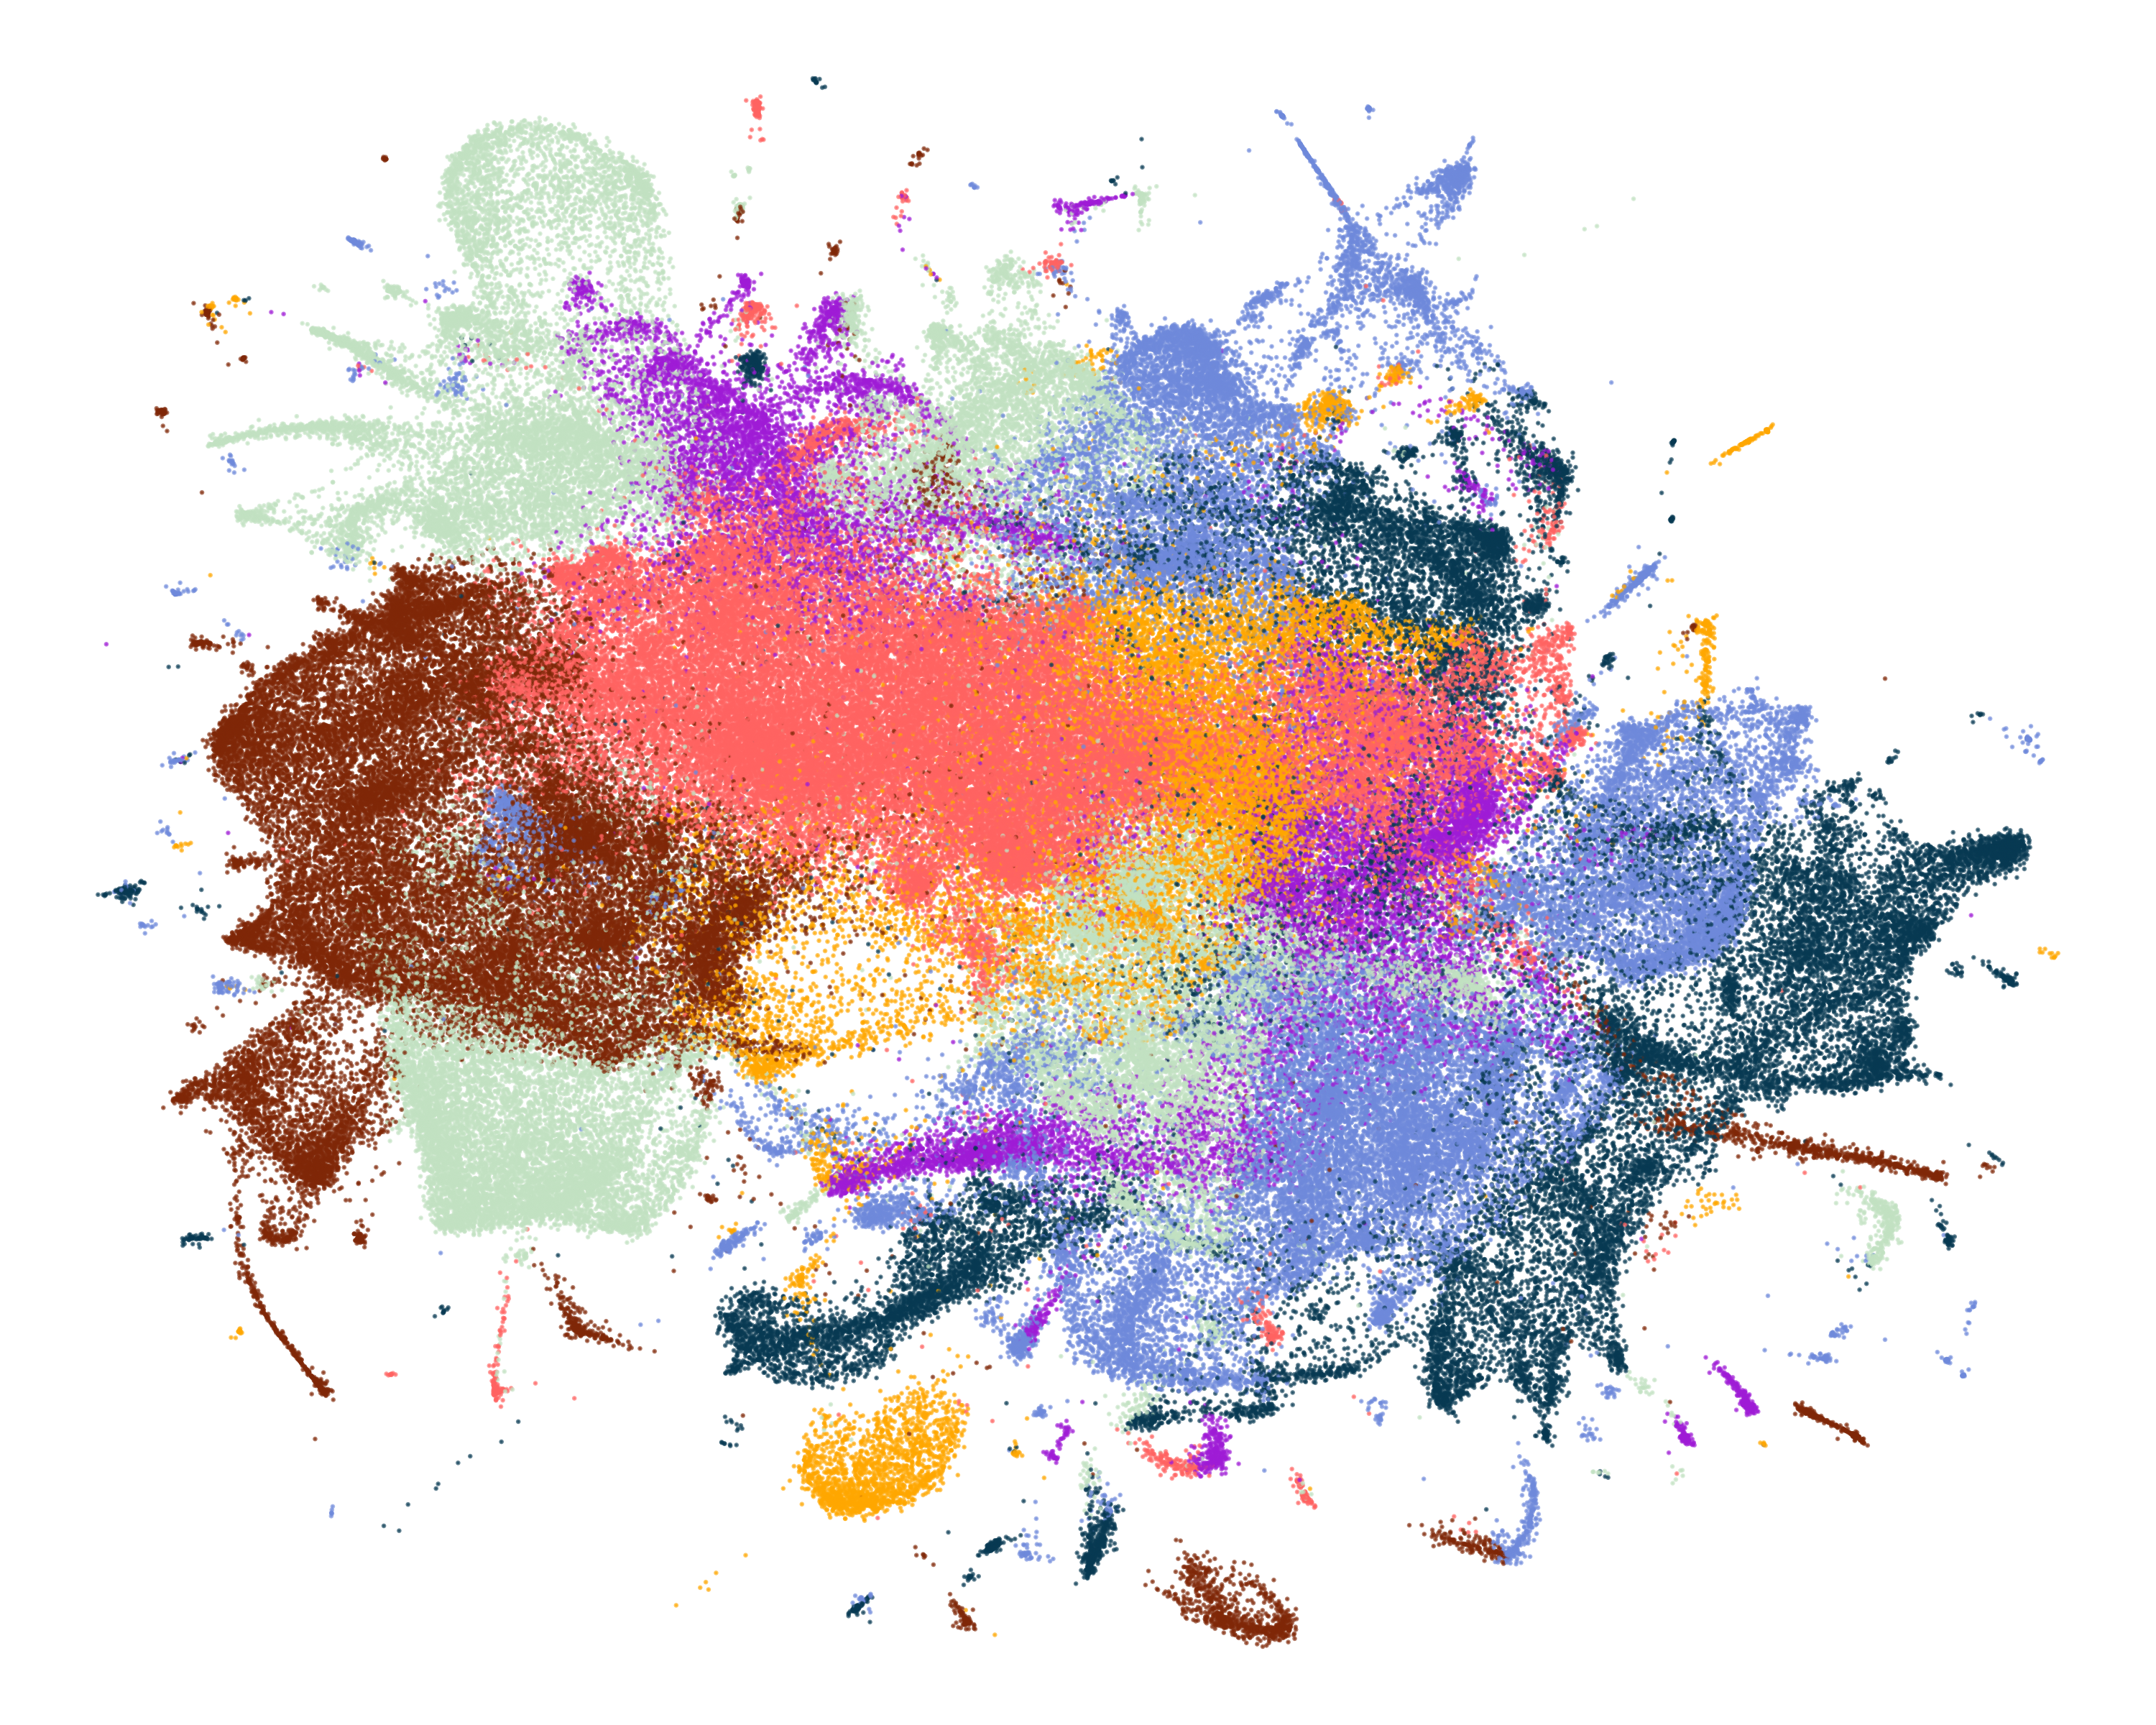
\includegraphics[width=7.03125in,height=\textheight]{img/ai_landscape_coloured.png}

}

\caption{Segmented Colourful Landscape Plot from an AI Landscape
Microsoft Project - Q2 FY24}

\end{figure}%

\section{Downstream Flourishes}\label{downstream-flourishes}

With the basics of each step covered, we will now touch on a few
potentially beneficial concepts worth grasping that may help us overcome
anything else that may occur when working within the Conversation
Landscape project domain.

\subsection{Model Saving \&
Reusability:}\label{model-saving-reusability}

Occasionally, a client may want us to track topics over time or perform
a landscape change analysis. In these cases, we need to save both our
Dimension Reduction and Clustering models so that new data can be
processed using these models, tp produce consistent and comparable
results.

This requires careful planning. When we initially reduce embeddings and
perform clustering, we use the \texttt{.fit()} method from
\texttt{sklearn} when either reducing the dimensions of or clustering on
the original embeddings. This ensures that the models are trained on the
data they are intended to represent, making future outputs comparable.

We had earlier, mentioned, that it is crucial to document the versions
of the modules and Python interpreter used. When we reduce or cluster
new data using our pre-fitted models, it is essential to do so with the
exact same versions of important libraries and Python. The reason is
that the internal representations and binary structures of the models
can differ between versions. If we attempt to load and apply previously
saved models with different versions, we risk encountering
incompatibility errors. By maintaining version control and documenting
the environment in which the models were created, we can ensure the
reusability of our models. Overall, this practice allows for us to be
accurate when tracking and comparing topics and noting any landscape
changes.

\subsection{Efficient Parameter
Tuning:}\label{efficient-parameter-tuning}

When we're performing certain steps within this workflow, more
specifically the Dimension Reduction with likes of UMAP, or if we were
to decide we'd want to cluster using HDBSCAN for example, being mindful
of and efficient with tuning the different parameters at each step will
definitely improve the outcome of our overall model. Therefore,
understanding these key parameters and how they can interact will
significantly enhance the performance of the techniques being used here.

\subsubsection{Dimension Reduction with
UMAP:}\label{dimension-reduction-with-umap}

n\_neighbors: This parameter controls the local neighborhood size used
in UMAP. A smaller value focuses more on capturing the local structure,
while a larger value considers more global aspects. Efficiently tuning
this parameter involves considering the nature of your data and the
scale at which you want to observe patterns.

min\_dist: The min distance argument determines quite literally how
tight our nodes are allowed to be positioned together within our
semantic space, a lower value for this will mean nodes will be tightly
packed together, whereas a higher number will ensure larger spacing of
data points.

n\_components: Here is where we decide how many dimensions we wish to
reduce our high-dimensional embeddings object down to, for visualisation
we will likely set this parameter to a value of 2.

\subsubsection{KMeans CLustering}\label{kmeans-clustering}

n\_clusters: KMeans is a relatively simple algorithm compared to other
methods and components, requiring very little input. Here we just
provide a value for the number of clusters we wish to form, this will
either be clusters in the embeddings or a smaller, more manageable
reduced embeddings object as mentiioned previously.

\subsubsection{HDBSCAN Clustering:}\label{hdbscan-clustering}

min\_samples: This parameter defines the minimum number of points
required to form a dense region. It helps determine the density
threshold for clusters and can determine how conservative we want the
clustering model to be. Put simply, a higher value can lead to fewer,
larger clusters, while a lower value can result in more, smaller
clusters.

min\_cluster\_size: This parameter sets the minimum size of clusters.
Like \texttt{min\_samples} it can directly influence the granularity of
the clustering results. In this case, smaller values allow the formation
of smaller clusters, while larger values prevent the algorithm from
identifying any small clusters(or those below the size of the provided
value). It's worth noting that the relationship between
\texttt{min\_samples} and \texttt{min\_cluster\_size} is crucial.
\texttt{min\_samples} should generally be less than or equal to
\texttt{min\_cluster\_size}. Adjusting these parameters in tandem helps
us to control the sensitivity of HDBSCAN, and for us to define what
qualifies as a cluster.

\subsubsection{Tip: Try starting with the default value for all of these
parameters, and incrementally adjust based on the desired granularity or
effect of any that we wish to
amend.}\label{tip-try-starting-with-the-default-value-for-all-of-these-parameters-and-incrementally-adjust-based-on-the-desired-granularity-or-effect-of-any-that-we-wish-to-amend.}

\subsection{Supporting Data
Visualisation:}\label{supporting-data-visualisation}

Once we have our landscape output, as shown in
\href{http://localhost:6377/conversation_landscape.html\#final-output-of-project}{Final
output of project}, we will inevitably need to display some further
information regarding our topics, most commonly; Volume over Time (VOT)
and Sentiment Distribution for each.

When doing so, we would ideally keep some formatting consistencies when
plotting, as we mentioned previously, the colouring of our topics must
remain the same throughout so that they match up with any previous
representations in existing visuals such as the landscape output. We
would also want to ensure that any plot we create orders our topics by
volume or at least in the same order throughout our project. We can
order our topics in terms of volume easily with just a few lines of
code.

First, we'll make sure to set the factor levels of our topics by using
\texttt{dplyr::count()} on the \texttt{topic\_name} column, and setting
the levels feature of the \texttt{factor()} base function based on the
counted output.

\begin{Shaded}
\begin{Highlighting}[]
\CommentTok{\# sort topics by order of volume}
\NormalTok{topic\_order }\OtherTok{\textless{}{-}}\NormalTok{ data }\SpecialCharTok{\%\textgreater{}\%}\NormalTok{ dplyr}\SpecialCharTok{::}\FunctionTok{count}\NormalTok{(topic\_name, }\AttributeTok{sort =} \ConstantTok{TRUE}\NormalTok{)}
\CommentTok{\# set levels determined by volume of topic, this orders the group variable for plotting}
\NormalTok{data }\OtherTok{\textless{}{-}}\NormalTok{ data }\SpecialCharTok{\%\textgreater{}\%} 
\NormalTok{  dplyr}\SpecialCharTok{::}\FunctionTok{mutate}\NormalTok{(}\AttributeTok{topic\_name =} \FunctionTok{factor}\NormalTok{(topic\_name, }\AttributeTok{levels =}\NormalTok{ topic\_order}\SpecialCharTok{$}\NormalTok{topic\_name))}
\end{Highlighting}
\end{Shaded}

\subsubsection{Topic Volume over Time}\label{topic-volume-over-time}

Starting with volume over time, we often choose to render a faceted plot
that includes all topics and their VOT for comparison. We can do so by
using functionality found in packages such as \texttt{JPackage} for
this.

\begin{Shaded}
\begin{Highlighting}[]
\CommentTok{\# plot topic volume over time using \textquotesingle{}plot\_group\_vol\_time()\textquotesingle{} function}
\NormalTok{data }\SpecialCharTok{\%\textgreater{}\%} 
\NormalTok{  JPackage}\SpecialCharTok{::}\FunctionTok{plot\_group\_vol\_time}\NormalTok{(}\AttributeTok{group\_var =}\NormalTok{ topic\_name,}
                                \AttributeTok{date\_var =}\NormalTok{ date,}
                                \AttributeTok{unit =} \StringTok{"day"}\NormalTok{,}
                                \AttributeTok{nrow =} \DecValTok{2}\NormalTok{) }\SpecialCharTok{+}
\NormalTok{  ggplot2}\SpecialCharTok{::}\FunctionTok{scale\_fill\_manual}\NormalTok{(}\AttributeTok{values =}\NormalTok{ topic\_colours) }\CommentTok{\# apply colours manually!}
\end{Highlighting}
\end{Shaded}

\includegraphics{conversation_landscape_files/figure-pdf/unnamed-chunk-7-1.pdf}

\subsubsection{Topic Sentiment
Distribution}\label{topic-sentiment-distribution}

Next, we might want/need to break each of our topics out by their
sentiment distribution to help shine light on any of particular interest
or to help us tell a more refined story using our topic model. This can
be done by using the \texttt{dr\_plot\_sent\_group()} function of the
\texttt{DisplayR} package.

\begin{Shaded}
\begin{Highlighting}[]
\NormalTok{data }\SpecialCharTok{\%\textgreater{}\%} 
\NormalTok{  DisplayR}\SpecialCharTok{::}\FunctionTok{dr\_plot\_sent\_group}\NormalTok{(}\AttributeTok{group\_var =}\NormalTok{ topic\_name,}
                               \AttributeTok{sentiment\_var =}\NormalTok{ sentiment,}
                               \StringTok{"percent"}\NormalTok{, }\AttributeTok{bar\_labels =} \StringTok{"none"}\NormalTok{, }
                               \AttributeTok{sentiment\_colours =} \FunctionTok{c}\NormalTok{(}\StringTok{"POSITIVE"} \OtherTok{=} \StringTok{"darkgreen"}\NormalTok{,}
                                                     \StringTok{"NEGATIVE"} \OtherTok{=} \StringTok{"darkred"}\NormalTok{))}
\end{Highlighting}
\end{Shaded}

\includegraphics{conversation_landscape_files/figure-pdf/unnamed-chunk-8-1.pdf}

\subsubsection{Alternative
Visualisations}\label{alternative-visualisations}

While the two visuals we have displayed so far are relatively basic and
commonly used, this does not mean that we won't require alternative
methods to display topic-level information. Often, we may render n-grams
per topic to display the relationships that exist between terms/phrases,
and we may create plots to showcase things such as data source or social
network/platform distributions across topics.

Finally, it's worth noting that the need for specific data visualisation
methods entirely depends on the project domain and brief, as well as any
outcomes/findings derived throughout. This means we ought to be flexible
in our approach to utilising any technique that may assist with
strengthening our understanding of the data and/or supporting our
analyses.

\part{Project work}

\chapter{A Data Science project}\label{a-data-science-project}

\section{What is a Data Science
project?}\label{what-is-a-data-science-project}

Aside from the obvious definition of a project (a piece of work planned
and executed to achieve a particular aim- in this case facilitate a
client's needs), what this section is referring to is the structure and
usage of a coding project.

\section{Where are projects
saved/located?}\label{where-are-projects-savedlocated}

All projects need to be saved onto the Google Drive. We have our own
Data Science section, where we save our project and internal work (code,
data, visualisations etc), which is in the filepath:

\texttt{Share\_Clients/data\_science\_project\_work/}

You should get access to this directory straight away.

Within the \texttt{data\_science\_project\_work} directory there are
subdirectories of all of our clients, such as
\texttt{data\_science\_project\_work/microsoft},
\texttt{data\_science\_project\_work/dyson} etc.

\begin{figure}[H]

{\centering \includegraphics{./img/drive_screenshot.png}

}

\caption{Screenshot of the \texttt{data\_science\_project\_work/}
directory with client-specific subdirectories}

\end{figure}%

\begin{tcolorbox}[enhanced jigsaw, colback=white, opacitybacktitle=0.6, coltitle=black, left=2mm, breakable, bottomtitle=1mm, toptitle=1mm, toprule=.15mm, colframe=quarto-callout-caution-color-frame, titlerule=0mm, title=\textcolor{quarto-callout-caution-color}{\faFire}\hspace{0.5em}{File paths}, colbacktitle=quarto-callout-caution-color!10!white, rightrule=.15mm, bottomrule=.15mm, arc=.35mm, opacityback=0, leftrule=.75mm]

You will see that we refer to the location of directories mainly by
their filepath, with the above screenshot of the Google Drive just for
full transparency and clarity.

There are no two ways about it, getting familiar with working with
filepaths in the command line (or in a script) is non-negotiable, but
will become second nature and you will be tab-completing filepaths in no
time at all!

\end{tcolorbox}

\section{RStudio Projects}\label{rstudio-projects}

We are primarily an \texttt{R} focused team, and as such we utilise
\href{https://support.posit.co/hc/en-us/articles/200526207-Using-RStudio-Projects}{RStudio
projects} to help keep all the files associated with a given project
together in one directory.

To create a RStudio Project, click File \textgreater{} New Project and
then follow the below steps, but call the directory the name of the
project (if a Microsoft project, appended by the project number) rather
than `r4ds'. Be sure to make sure the option `Create project as
subdirectory of' is the client directory on the Drive (in the case of
Microsoft, this is
\texttt{Share\_Clients/data\_science\_project\_work/microsoft/project\_work/}).

\begin{figure}[H]

{\centering \includegraphics{./img/new_project_workflow.png}

}

\caption{Steps to create a new project, taken from R for Data Science
(2e) https://r4ds.hadley.nz/workflow-scripts.html\#projects}

\end{figure}%

Once this process is complete, there should be a new project folder in
the client directory, with a \texttt{.Rproj} file within it.

If this is your first time using RStudio Projects, we recommend reading
\href{https://r4ds.hadley.nz/workflow-scripts.html\#projects}{this
section within the R for Data Science book}, to familiarise yourself
with some more intricacies of Project work within R (such as relative
and absolute paths) which we would not do justice summarising here.

\section{Components of a DS project}\label{components-of-a-ds-project}

DS projects consist of a parent project directory, with an associated
\texttt{.Rproj} file, and three compulsory subdirectories \texttt{code},
\texttt{data}, and \texttt{viz} (all of which are made manually).

\begin{center}
\includegraphics[width=0.4\textwidth,height=\textheight]{./img/project_directory.png}
\end{center}

Whilst there are no prizes for what goes in each subdirectory, it can be
useful to have a structure in place to facilitate workflow ease.

\subsubsection{\texorpdfstring{\texttt{code}}{code}}\label{code}

Within the \texttt{code} subdirectory is where all scripts should be
kept. We utilise \texttt{.Rmd} (R Markdown) documents rather than basic
\texttt{.R} scripts for our code.

We do this for a few reasons, but the main benefits include:

\begin{itemize}
\tightlist
\item
  It acts as an environment in which to do data science- we can capture
  not only what we did, but importantly \emph{why} we did it
\item
  We can easily build and export a variety of different output formats
  from a R Markdown document (PDF, HTML, slideshow etc)
\end{itemize}

As part of our commitment to literate programming, there are some good
practices that we can implement at this level of abstraction.

Firstly, do not have extremely long \texttt{.Rmd} documents, as this is
no good for anybody. Instead split up your documents into different
sections based on the purpose of the code.

Whilst this can be a bit subjective, a good rule of thumb is to have a
separate \texttt{.Rmd} for each aspect of a workflow. For example, we
might have one \texttt{.Rmd} for reading in raw data, another for
cleaning the data, another for EDA, and another for performing topic
modelling etc.

We should also follow the
\href{https://style.tidyverse.org/index.html}{tidyverse style guide} in
the naming of files, which states:

\begin{quote}
If files should be run in a particular order, prefix them with numbers
\end{quote}

Therefore it makes sense to prefix our files, as we must load in the raw
data before we can clean the data, and we must clean the data before we
can perform certain analyses etc.

So we might have something like \texttt{00\_load\_data.Rmd},
\texttt{01\_clean\_data.Rmd}, \texttt{02\_topic\_modelling.Rmd}.

\subsubsection{\texorpdfstring{\texttt{data}}{data}}\label{data}

\texttt{data} is where we save any data file that comes from a project.

The vast majority of projects will involve analysing an export from a
social listening platform, such as Sprinklr. Analysts will save the
export in the form of \texttt{.csv} or \texttt{.xlsx} files on the Drive
(not within the Data Science section). As Sprinklr limits its exports to
10k rows of data per export file, we often are presented with 10s/100s
of files with raw mentions. Therefore once we read these files into R,
it is a good opportunity to save them as an \texttt{.Rds} in the
\texttt{code} folder using the function \texttt{write\_rds()} to avoid
having to reread the raw excel or csv files in again.

It is within \texttt{data} where you would also save cleaned datasets
and the outputs of different analyses (not visualisations though). This
is not limited to \texttt{.Rds} files, but could also be word documents,
excel spreadsheets etc.

As projects get more complex with many analyses, it can be easy to
clutter this subdirectory. As such, it is recommended to make folders
within \texttt{data} to help maintain structure. This means it is easy
to navigate where cleaned data is because it will be in a folder such as
\texttt{data/cleaned\_data} and a dataframe with topic labels would be
in \texttt{data/topic\_modelling}.

\begin{tcolorbox}[enhanced jigsaw, colback=white, opacitybacktitle=0.6, coltitle=black, left=2mm, breakable, bottomtitle=1mm, toptitle=1mm, toprule=.15mm, colframe=quarto-callout-tip-color-frame, titlerule=0mm, title=\textcolor{quarto-callout-tip-color}{\faLightbulb}\hspace{0.5em}{Save liberally}, colbacktitle=quarto-callout-tip-color!10!white, rightrule=.15mm, bottomrule=.15mm, arc=.35mm, opacityback=0, leftrule=.75mm]

Generally speaking, space is cheaper than time. If in doubt, save an
intermediate dataframe after an analysis if you \emph{think} you'll need
it in the future. It is better to run an analysis once and save the
output to never look at it again, than to run an analysis, not save the
output, and then need to rerun the analysis the following week.

\end{tcolorbox}

\subsubsection{\texorpdfstring{\texttt{viz}}{viz}}\label{viz}

Any visualisation that is made throughout the project should be saved
here. Again, this directory should be split into separate folders to
keep different analyses separate, navigable, and clear. This is
especially useful if there is are visualisations being made of the same
analysis mapped over different variables or parameters, or if the
project involves the analysis of separate products or brands.

For example, the below shows a screenshot of a \texttt{viz} folder for a
project that looked at three products. Within \texttt{viz} the plots for
each brand are in their own folder, and within each brand
(\texttt{chatgpt}, \texttt{copilot}, \texttt{gemini}) there are further
folders to split up the type of visualisations created
(\texttt{area\_charts}, \texttt{eda} etc), with even a third level of
subdirectory (\texttt{area\_charts/peaks} and
\texttt{area\_charts/pits}).

\begin{figure}[H]

{\centering \includegraphics[width=0.4\textwidth,height=\textheight]{./img/viz_directory.png}

}

\caption{Example viz directory hierarchy for a Peaks and Pits project}

\end{figure}%

\chapter{Project key players}\label{project-key-players}

\section{Insights Analyst}\label{insights-analyst}

Analysts add the bit of human-insight sparkle to our projects. They work
closely with the client and stakeholder to help frame our findings so
they are suitable for the clients business needs. At a high level, we
may say ``Our clustering analysis identified five distinct regions of
conversation based on the semantics of the language used'' whereas an
analyst would translate that to ``We have five key conversational themes
that can be targeted with tailored marketing strategies to boost product
reach on socials''. Though this does vary on a project by project basis
and we often have to act as a conduit between the science and the client
too.

Insight analysts are who work closely with Sprinklr and other social
listening platforms to obtain the data we analyse. They will craft
queries to pull the relevant data from a variety of sources and save the
data on the Drive for us to access and do science on.

\section{Account Manager}\label{account-manager}

Account Managers (AMs) are the point of contact between our business and
the client, bridging the gap between the technical teams (in our cases
DS or Insights) and the client/stakeholder. They will arrange meetings
with the client, help us understand the client's needs and business
objectives, and coordinate project logistics, timelines, and
deliverables. As project deadlines approach, account managers will help
QA our deliveries (normally in the form of a PowerPoint or Keynote
presentation), providing valuable opinion from a non-technical
background (it can be easy for us to get stuck in the weeds and forget
that stakeholders do not know as much about data as we do). Broadly, AMs
make sure both us as a company, and the client, are held accountable for
the work we are contracted to do.

\section{Data/Insight Director}\label{datainsight-director}

Depending on the project, there will be a Data Director or Insight
Director involved on the project too. You will notice that they will
normally be resources on Float Whilst not working on the nitty gritty of
the project, they are there to help steer the project in the appropriate
direction based on the clients business needs. They will also be
checking the final delivery as it is created, making sure the
deliverables and story we have thread is suitable and valid.

\part{Development}

\chapter{Our Packages}\label{our-packages}

We have a suite of R packages that have been developed internally. They
all serve different purposes on a project, but together aim to empower
the SAMY Alliance. We don't license the software to clients. What we
sell is the knowledge that they can produce.

\section{\texorpdfstring{\href{https://parser.shareldn.com/index.html}{ParseR}}{ParseR}}\label{parser}

\includegraphics[width=0.2\textwidth,height=\textheight]{./img/hex/parser.png}

ParseR is the collective name for the techniques SAMY uses for text
analysis. It's primarily based on the tidytext philosophy and the
analysis is normally carried out in R.

\section{\texorpdfstring{\href{https://avery-island.github.io/ConnectR/index.html}{ConnectR}}{ConnectR}}\label{connectr}

\includegraphics[width=0.2\textwidth,height=\textheight]{./img/hex/connectr.png}

ConnectR is our package for network analysis. It helps the user find
important individuals by graphing retweets and important communities by
graphing mentions.

\section{\texorpdfstring{\href{https://avery-island.github.io/SegmentR/index.html}{SegmentR}}{SegmentR}}\label{segmentr}

\includegraphics[width=0.2\textwidth,height=\textheight]{./img/hex/segmentr.png}

SegmentR is the collective name for the techniques SAMY uses to find
latent groups in data.

\section{\texorpdfstring{\href{https://aoiferyan-sc.github.io/BertopicR/articles/manipulating-the-model.html}{BertopicR}}{BertopicR}}\label{bertopicr}

BertopicR is our package which allows access to
\href{https://maartengr.github.io/BERTopic/index.html}{BERTopic's}
modelling suite in \texttt{R} via \texttt{reticulate}.

\section{\texorpdfstring{\href{https://github.com/jpcompartir/LandscapeR}{LandscapeR}}{LandscapeR}}\label{landscaper}

\includegraphics[width=0.2\textwidth,height=\textheight]{./img/hex/landscaper.png}

LandscapeR is our package for exploring text data which has been
transformed into a navigable landscape. The package makes use of
cutting-edge language models and their dense word embeddings,
dimensionality reduction techniques, clustering and/or topic modelling
as well as Shiny for an interactive data-exploration \& cleaning UI.

If the conversation has been mapped appropriately, you will find that
mentions close together in the Shiny application/UMAP plot have similar
meanings, posts far apart have less similar meanings. This makes it
possible to understand and explore thousands, hundreds of thousands, or
even millions of posts at a level which was previously impossible.

\section{\texorpdfstring{\href{https://github.com/jpcompartir/LimpiaR}{LimpiaR}}{LimpiaR}}\label{limpiar}

\includegraphics[width=0.2\textwidth,height=\textheight]{./img/hex/limpiar.png}

LimpiaR is an R library of functions for cleaning \& pre-processing text
data. The name comes from `limpiar' the Spanish verb'to clean'.
Generally when calling a LimpiaR function, you can think of it as
`clean\ldots{}'.

LimpiaR is primarily used for cleaning unstructured text data, such as
that which comes from social media or reviews. In its initial release,
it is focused around the Spanish language, however, some of its
functions are language-ambivalent.

\section{\texorpdfstring{\href{https://jpcompartir.github.io/DisplayR/}{DisplayR}}{DisplayR}}\label{displayr}

DisplayR is our package for data visualization, offering a wide array of
functions tailored to meet various data visualization needs. This
versatile package aims to improve data presentation and communication by
providing visually engaging and informative graphics.

\section{\texorpdfstring{\href{https://avery-island.github.io/HelpR/index.html}{HelpR}}{HelpR}}\label{helpr}

\includegraphics[width=0.2\textwidth,height=\textheight]{./img/hex/helpr.png}

HelpR is SAMY's R package for miscellaneous functions that can come in
handy across a variety of workflows.

As you progress through your data science journey, you may take an
interest in developing your own package. Depending on your previous
experience developing software, this might be daunting, but don't worry
none of us had much experience building packages when we joined; we all
learned on the job - and so can you. If you want to.

See the \href{package_development.qmd}{Package Development} document for
more information.

\chapter{Package Development}\label{package-development}

One of the beautiful things about Data Science at SAMY is that you get
to choose your path between research, development, or a hybrid. If
you're reading this, you've probably decided that you want to explore
some development - what better way to start than building your own
package?

\begin{tcolorbox}[enhanced jigsaw, colback=white, opacitybacktitle=0.6, coltitle=black, left=2mm, breakable, bottomtitle=1mm, toptitle=1mm, toprule=.15mm, colframe=quarto-callout-note-color-frame, titlerule=0mm, title=\textcolor{quarto-callout-note-color}{\faInfo}\hspace{0.5em}{Note}, colbacktitle=quarto-callout-note-color!10!white, rightrule=.15mm, bottomrule=.15mm, arc=.35mm, opacityback=0, leftrule=.75mm]

For a high-level overview of our existing packages, refer to the
\href{packages.qmd}{our packages} document.

\end{tcolorbox}

We build packages because they are convenient ways to share our code \&
data and democratise access to our tools \& workflows - besides, that
Google Doc of functions is getting heavy, and copying \& pasting code
from project to project is getting tiresome. Eventually you'll want the
familiar \texttt{library()} syntax.

Historically our packages have been built in R for two key reasons:

\begin{enumerate}
\def\labelenumi{\arabic{enumi}.}
\tightlist
\item
  The profile/experience of people in the team
\item
  The ecosystem for building packages is well-maintained and documented
\end{enumerate}

In recent times we have moved to more of a hybrid approach between R \&
Python - the former we find to be considerably more easy to use for data
wrangling and visualisation, and the latter for modelling and anything
to do with LLMs. Internal development for Python has lagged behind R,
but we expect this to change over time as we seek to be tool agnostic
and focus on the right tool for the job at hand.

\begin{tcolorbox}[enhanced jigsaw, colback=white, opacitybacktitle=0.6, coltitle=black, left=2mm, breakable, bottomtitle=1mm, toptitle=1mm, toprule=.15mm, colframe=quarto-callout-note-color-frame, titlerule=0mm, title=\textcolor{quarto-callout-note-color}{\faInfo}\hspace{0.5em}{Reticulate}, colbacktitle=quarto-callout-note-color!10!white, rightrule=.15mm, bottomrule=.15mm, arc=.35mm, opacityback=0, leftrule=.75mm]

Reticulate is an R package that allows us to import Python packages and
functions in R. Currently this is a one-way street - we can't use
reticulate to import R functions and packages. This has impacted our
decision in the past, e.g.~with BertopicR. We envisioned Insight
Analysts using BertopicR as a drop-in or replacement for topic modelling
with SegmentR. Weighing up the additional difficulty in development vs
the time and resource necessary for Analysts to learn Python as well as
R, we opted for reticulate.

Using reticulate requires managing Python environments from R, this
leads to difficulties of its own.

\end{tcolorbox}

\chapter{R}\label{r}

Here we'll look at how to get off the ground in R using the R package
stack - \{usethis\}, \{pkgdown\}, \{devtools\}, \{testthat\} and
\{roxygen2\}.

\section{Building your own package}\label{building-your-own-package}

The (nearly) DIY way:

This check-list should get you \textbf{most of the way} there, but it's
always possible that we've forgotten something or there has been a
disturbance in the force a change in the package ecosystem. When this
happens, open up an issue or submit a PR and help the next person who
comes along.

\begin{itemize}
\tightlist
\item[$\square$]
  Create a new repository on GitHub
\item[$\square$]
  Clone the repository
\end{itemize}

\begin{tcolorbox}[enhanced jigsaw, colback=white, opacitybacktitle=0.6, coltitle=black, left=2mm, breakable, bottomtitle=1mm, toptitle=1mm, toprule=.15mm, colframe=quarto-callout-tip-color-frame, titlerule=0mm, title=\textcolor{quarto-callout-tip-color}{\faLightbulb}\hspace{0.5em}{Folder management}, colbacktitle=quarto-callout-tip-color!10!white, rightrule=.15mm, bottomrule=.15mm, arc=.35mm, opacityback=0, leftrule=.75mm]

Create a folder at your home directory named `git\_repos' and store all
of your repositories here:

\end{tcolorbox}

\begin{itemize}
\tightlist
\item[$\square$]
  Open RStudio and call \texttt{usethis::create\_package()}
\item[$\square$]
  \texttt{usethis::use\_git()} in the console and commit files
\item[$\square$]
  Check git has been set up with \texttt{usethis::git\_sitrep()} (or
  \texttt{git\ status} in the terminal)
\item[$\square$]
  Set an upstream branch
  e.g.~\texttt{git\ remote\ add\ upstream\ \textless{}link\_to\_repo\_main\textgreater{}}
  in the terminal
\item[$\square$]
  \texttt{usethis::use\_vignette()} to add a vignettes folder and start
  your first vignette
\item[$\square$]
  Add individual functions/scripts with \texttt{use\_r("script\_name")}
  - these appear in your R/ folder
\item[$\square$]
  Document each function following roxygen2's structure
  \hyperref[roxygen2-gl]{Roxygen2 guidelines}
\item[$\square$]
  Call \texttt{use\_package()} whenever you use an external package
  inside your package.
\end{itemize}

\begin{tcolorbox}[enhanced jigsaw, colback=white, opacitybacktitle=0.6, coltitle=black, left=2mm, breakable, bottomtitle=1mm, toptitle=1mm, toprule=.15mm, colframe=quarto-callout-tip-color-frame, titlerule=0mm, title=\textcolor{quarto-callout-tip-color}{\faLightbulb}\hspace{0.5em}{DESCRIPTION}, colbacktitle=quarto-callout-tip-color!10!white, rightrule=.15mm, bottomrule=.15mm, arc=.35mm, opacityback=0, leftrule=.75mm]

Your package will now have a DESCRIPTION file, add external packages
your package requires to Imports. Add additional packages used in
vignettes to Suggests. - But be careful, it's generally not advisable to
use packages just for vignettes!

You can use the \texttt{usethis::use\_latest\_dependencies()} to add
recent versions to your packages, but beware this can be restrictive.
Ideally you would add the minimum package version necessary to run your
code.

\end{tcolorbox}

\begin{itemize}
\tightlist
\item[$\square$]
  \texttt{usethis::use\_*\_license()} - default to
  usethis::use\_mit\_license()
\item[$\square$]
  \texttt{usethis::use\_testthat()} and
  \texttt{use\_test("script\_name")} to start writing units tests for
  your functions and add testthat to suggests.
\item[$\square$]
  Call \texttt{usethis::use\_readme\_rmd()} to allow for markdown code
  chunks in your readme - just remember to
  \texttt{devtools::build\_readme()} when you're done.
\item[$\square$]
  Call \texttt{usethis::use\_news\_md()}
\item[$\square$]
  When you're ready to add a website, call
  \texttt{usethis::use\_pkgdown()} \texttt{pkgdown::init\_site()},
  \texttt{pkgdown::build\_home\_index()},
  \texttt{pkgdown::build\_search()},
  \texttt{pkgdown::build\_reference()},
  \texttt{pgkdown::build\_articles()}, and then
  \texttt{pkgdown::build\_site()}
\item[$\square$]
  Add each function to pkgdown.yml's reference section (we recommend
  viewing a working yml file from one of the other packages to get you
  started).
\end{itemize}

The Easy Way (Tidy functions) Read through the
\href{https://usethis.r-lib.org/articles/usethis-setup.html}{usethis-setup
guide} and then use the \texttt{usethis::create\_tidy\_package()} to
create a package with some guardrails.

\begin{tcolorbox}[enhanced jigsaw, colback=white, opacitybacktitle=0.6, coltitle=black, left=2mm, breakable, bottomtitle=1mm, toptitle=1mm, toprule=.15mm, colframe=quarto-callout-tip-color-frame, titlerule=0mm, title=\textcolor{quarto-callout-tip-color}{\faLightbulb}\hspace{0.5em}{Guardrails or no guardrails?}, colbacktitle=quarto-callout-tip-color!10!white, rightrule=.15mm, bottomrule=.15mm, arc=.35mm, opacityback=0, leftrule=.75mm]

The \texttt{usethis::create\_tidy\_package()} function is a helpful
abstraction, but it will be better for your long-term development if you
know how to do this stuff without the abstraction. That way, when you
need to fix something, or do something slightly different than the
prescribed way, you'll have a better chance of success.

\end{tcolorbox}

Want to go deeper? Check out the \href{https://r-pkgs.org/}{R Packages
Book}, we recommend skimming first and then using it as a reference
manual.

\section{Development workflow}\label{development-workflow}

Once you've built the package there are some things you will want to do
regularly to ensure your package stays in good shape. This is by no
means an exhaustive list - be sure to add your tips \& tricks as you
amass them.

\includegraphics{img/bernie.png}

\begin{itemize}
\tightlist
\item[$\square$]
  Run \texttt{testthat::test\_package()} often to check for regressions
  in your code
\item[$\square$]
  Run \texttt{devtools::check()} occasionally to make sure you haven't
  made any obvious mistakes - try to keep notes, warnings and errors to
  0!
\item[$\square$]
  Use \texttt{devtools::load\_all()} to reload the package when you've
  made changes. (\texttt{devtools::document()} also calls
  \texttt{load\_all()} when called)
\item[$\square$]
  Run \texttt{roxygen2::roxygenise(clean\ =\ TRUE)} if your
  documentation doesn't look as you expect after
\item[$\square$]
  Use \texttt{pkgdown::build\_site()} when you expect to see changes in
  your package's website
\item[$\square$]
  Use \texttt{pkgdown::clean\_site()} and
  \texttt{pkgdown::build\_site()} when expected changes aren't
  reflecting in your preview
\end{itemize}

\section{Contributing to existing
packages}\label{contributing-to-existing-packages}

\begin{itemize}
\item[$\square$]
  Pull current state of repo/package from origin
\item[$\square$]
  Create a new branch, can use \texttt{usethis::pr\_init()} from usethis
  to make this a bit easier, otherwise
  \texttt{git\ checkout\ -b\ "branch\_name"}
\item[$\square$]
  Run \texttt{devtools::test()} \texttt{devtools::check()} at regular
  intervals, keep errors, warnings, notes down to minimum
\item[$\square$]
  Build out logic for new changes, add to R/ where necessary.
  \texttt{usethis::use\_r()} function to add new scripts properly
\item[$\square$]
  Build out tests for new logic in tests/
\item[$\square$]
  Ensure function-level documentation is added to any new logic,
  including @title, @description, @details, @param, @returns, @examples
  and @export if function is to be exported, or @internal otherwise. Let
  roxygen2 take care of @usage.
\item[$\square$]
  Keep re-running tests and check!
\item[$\square$]
  If you're introducing something new, update package-level
  documentation e.g.~vignettes and/or readme explaining what you've
  introduced and how it should be used. Provide examples where possible.
  If you're building out a new capability you may need a whole new
  vignette, use the \texttt{usethis::use\_vignette()} function.
\end{itemize}

\begin{tcolorbox}[enhanced jigsaw, colback=white, opacitybacktitle=0.6, coltitle=black, left=2mm, breakable, bottomtitle=1mm, toptitle=1mm, toprule=.15mm, colframe=quarto-callout-tip-color-frame, titlerule=0mm, title=\textcolor{quarto-callout-tip-color}{\faLightbulb}\hspace{0.5em}{What are vignettes?}, colbacktitle=quarto-callout-tip-color!10!white, rightrule=.15mm, bottomrule=.15mm, arc=.35mm, opacityback=0, leftrule=.75mm]

Vignettes are long-form guides that provide in-depth documentation for
your package. They go beyond the basic function documentation and
explain how to use the package to solve specific problems, often with
detailed examples and code. Vignettes showcase your package's full range
of capabilities and help users understand how to effectively utilise its
features

\end{tcolorbox}

\begin{itemize}
\item[$\square$]
  If you're updating legacy code, check that vignettes are up-to-date
  with the changes you've made - we want to avoid code-documentation
  drift where possible.
\item[$\square$]
  Add your function to the reference section in \_pkgdown,yml if it's
  being exported.
\item[$\square$]
  Add data objects, \texttt{.Rhistory}, \texttt{*.Rproj},
  \texttt{.Rprofile}, \texttt{.DS\_Store}, to \texttt{.gitignore}
\item[$\square$]
  Run \texttt{pkgdown::clean\_site()} and
  \texttt{pkgdown::build\ site()}, visually inspect each section of the
  site
\end{itemize}

Pull request when ready.

\subsection{Code}\label{code-1}

Generally code should sit in the R/ folder, you can choose between a
script per function or use scripts as modules, where a module is a
particular use case, or logical unit. Historically we sided on the
former, but as a package grows it can become difficult to
manage/navigate, and there can be a decoupling of logic. Ultimately this
is a matter of taste in R.

\subsubsection{Exercises - code}\label{exercises---code}

\begin{tcolorbox}[enhanced jigsaw, colback=white, opacitybacktitle=0.6, coltitle=black, left=2mm, breakable, bottomtitle=1mm, toptitle=1mm, toprule=.15mm, colframe=quarto-callout-warning-color-frame, titlerule=0mm, title=\textcolor{quarto-callout-warning-color}{\faExclamationTriangle}\hspace{0.5em}{Exercises}, colbacktitle=quarto-callout-warning-color!10!white, rightrule=.15mm, bottomrule=.15mm, arc=.35mm, opacityback=0, leftrule=.75mm]

You may need to consult external resources to answer the exercises,
we've tried to provide links to help you along the way, but we encourage
you to embrace the joy of discovery and find relevant sources/fill in
the gaps where necessary!

\end{tcolorbox}

\begin{enumerate}
\def\labelenumi{\arabic{enumi}.}
\tightlist
\item
  What are the practical differences between \texttt{.gitignore} and
  \texttt{.Rbuildignore}?
\end{enumerate}

\begin{itemize}
\tightlist
\item
  What objects should go in \texttt{.gitignore} but not
  \texttt{.Rbuildignore}, and vice versa?
\end{itemize}

\begin{enumerate}
\def\labelenumi{\arabic{enumi}.}
\setcounter{enumi}{1}
\tightlist
\item
  What does the DESCRIPTION file do?
\item
  Write your own description for each of the following packages,
  detailing what they are for where they sit in the R package stack:
\end{enumerate}

\begin{itemize}
\tightlist
\item[$\square$]
  testthat
\item[$\square$]
  roxygen2
\item[$\square$]
  devtools
\item[$\square$]
  pkgdown
\item[$\square$]
  usethis
\end{itemize}

\subsection{Tests}\label{tests}

\begin{quote}
In a perfect world, every dog implementation detail would have a home
test and every home test would have an implementation detail.
\end{quote}

There is a balance to be struck between testing \emph{absolutely
everything} and testing what needs to be tested. Before we get into the
finer details, let's establish why we're writing tests in the first
place. The first reason for writing tests is to help you write software
that works. The second reason is to help you do this fast, and with
confidence.

Testing is not to prove that your code has no bugs, or cannot have any
bugs in the future. Whenever you do find a bug, or someone reports one,
write a test as you fix the issue.

For more information and another opinion, check out the
\href{https://r-pkgs.org/testing-basics.html}{R Packages testing
section}, and the \href{testing.qmd}{Testing document}

\begin{tcolorbox}[enhanced jigsaw, colback=white, opacitybacktitle=0.6, coltitle=black, left=2mm, breakable, bottomtitle=1mm, toptitle=1mm, toprule=.15mm, colframe=quarto-callout-tip-color-frame, titlerule=0mm, title=\textcolor{quarto-callout-tip-color}{\faLightbulb}\hspace{0.5em}{Tip}, colbacktitle=quarto-callout-tip-color!10!white, rightrule=.15mm, bottomrule=.15mm, arc=.35mm, opacityback=0, leftrule=.75mm]

Don't let testing paralyse your development process, they're there to
help not hinder. As a rule-of-thumb, if your tests for a function are
more complex than your function, you've gone too far.

\end{tcolorbox}

\subsection{Documentation}\label{documentation}

We use \{roxygen2\} tags to document our functions. Visit the
\href{https://roxygen2.r-lib.org/articles/rd.html}{documenting
functions} article for a primer.

Using the roxygen2 skeleton promotes consistent documentation, check out
a function's help page (e.g.~\texttt{?ParseR::count\_ngram}) to see how
rendered documentation looks - do this regularly with your own
functions.

We tend to find our documentation could always be better, more complete.
You can't hope to cover \textbf{everything} a user could do with your
function, but make sure it's clear from the documentation what your
function is for and what its primary uses are.

\includegraphics{img/parser_documentation.png}

\begin{tcolorbox}[enhanced jigsaw, colback=white, opacitybacktitle=0.6, coltitle=black, left=2mm, breakable, bottomtitle=1mm, toptitle=1mm, toprule=.15mm, colframe=quarto-callout-warning-color-frame, titlerule=0mm, title=\textcolor{quarto-callout-warning-color}{\faExclamationTriangle}\hspace{0.5em}{Warning}, colbacktitle=quarto-callout-warning-color!10!white, rightrule=.15mm, bottomrule=.15mm, arc=.35mm, opacityback=0, leftrule=.75mm]

Most people will scroll straight past the @description and @details and
go directly to your code examples.

\end{tcolorbox}

\subsubsection{Guidelines for commonly-used Roxygen
tags}\label{roxygen2-gl}

\begin{longtable}[]{@{}
  >{\raggedright\arraybackslash}p{(\columnwidth - 2\tabcolsep) * \real{0.2778}}
  >{\raggedright\arraybackslash}p{(\columnwidth - 2\tabcolsep) * \real{0.7222}}@{}}
\toprule\noalign{}
\begin{minipage}[b]{\linewidth}\raggedright
Tag
\end{minipage} & \begin{minipage}[b]{\linewidth}\raggedright
Description
\end{minipage} \\
\midrule\noalign{}
\endhead
\bottomrule\noalign{}
\endlastfoot
@title & One-line description of what your function does \\
@description & A paragraph elaborating on your title \\
@details & A more detailed description of the function e.g.~explaining
how its arguments interact, or other key implementation details. \\
@param & A description of the function's parameters \\
@return & A description of the function's return value \\
@examples & Examples of how to use the function \\
@export & Whether the function is exported or not \\
\end{longtable}

\subsubsection{Exercises -
Documentation}\label{exercises---documentation}

\begin{enumerate}
\def\labelenumi{\arabic{enumi}.}
\tightlist
\item
  What is the title of \{dplyr\}'s \texttt{mutate()} function?
\item
  @examples must be self-contained, create an example that is not
  self-contained, and one that is.
\item
  Which package(s) (any programming language) stick out in your mind as
  being well-documented and easy to use, what did the creators do well?
\item
  Audit SAMY's R packages, find a function with sub-par documentation
  and upgrade it. Then fire in a Pull Request!
\end{enumerate}

\subsection{Data}\label{data-1}

You're probably going to need some package-level data for your @examples
or your vignettes. Before going off and finding or creating a new data
set:

\begin{enumerate}
\def\labelenumi{\arabic{enumi}.}
\tightlist
\item
  Check whether you can demonstrate what you need with existing datasets
  - call \texttt{data()} in your console
\item
  Make sure the dataset you have chosen comes from a package your
  package explicitly Imports or Suggests
\end{enumerate}

If you still can't find the right dataset, create one!

\begin{enumerate}
\def\labelenumi{\arabic{enumi}.}
\tightlist
\item
  Load the dataset into memory
\item
  Call \texttt{usethis::use\_data(dataset\_variable\_name)}
\item
  Document the columns
\end{enumerate}

If you choose this route, some interesting problems may lie in wait.
Skip to Exercises 1.

To go deeper view the \href{https://r-pkgs.org/data.html}{R Packages
Dataset Section}

Datasets from the \{datasets\} package come with base R

\subsubsection{Exercises - Data}\label{exercises---data}

\begin{enumerate}
\def\labelenumi{\arabic{enumi}.}
\tightlist
\item
  Why might you add your data artefacts to \texttt{.Rbuildignore} or
  \texttt{.gitignore}?
\item
  Which package does the \texttt{diamonds} dataset ship with?
\end{enumerate}

You're probably going to need some data\ldots{} existing data\ldots{}
adding new usethis::use\_data() usethis::use\_data\_raw()

\subsection{Website}\label{website}

pkgdown .nojekyll

\subsubsection{Exercises - Website}\label{exercises---website}

\begin{enumerate}
\def\labelenumi{\arabic{enumi}.}
\tightlist
\item
  Explain in your own words what .nojekyll is for.
\end{enumerate}

\begin{itemize}
\tightlist
\item
  Where should it be placed in your package?
\item
  What problems arise when you don't have one?
\end{itemize}

\begin{enumerate}
\def\labelenumi{\arabic{enumi}.}
\setcounter{enumi}{1}
\tightlist
\item
\end{enumerate}

\chapter{Python}\label{python}

\begin{tcolorbox}[enhanced jigsaw, colback=white, opacitybacktitle=0.6, coltitle=black, left=2mm, breakable, bottomtitle=1mm, toptitle=1mm, toprule=.15mm, colframe=quarto-callout-warning-color-frame, titlerule=0mm, title=\textcolor{quarto-callout-warning-color}{\faExclamationTriangle}\hspace{0.5em}{Warning}, colbacktitle=quarto-callout-warning-color!10!white, rightrule=.15mm, bottomrule=.15mm, arc=.35mm, opacityback=0, leftrule=.75mm]

This document is very much a work in progress, key steps may be missing.

\end{tcolorbox}

\section{Folder Setup}\label{folder-setup}

The first step in creating a Python package is setting up the project
structure. Create a new directory for your project and organize it with
the following subdirectories and files:

\begin{itemize}
\tightlist
\item[$\square$]
  your\_package\_name/: The main package directory containing your
  Python modules and code. Make sure to add a \texttt{\_\_init\_\_.py}
  file to the source and any modules.
\end{itemize}

\begin{tcolorbox}[enhanced jigsaw, colback=white, opacitybacktitle=0.6, coltitle=black, left=2mm, breakable, bottomtitle=1mm, toptitle=1mm, toprule=.15mm, colframe=quarto-callout-tip-color-frame, titlerule=0mm, title=\textcolor{quarto-callout-tip-color}{\faLightbulb}\hspace{0.5em}{\textbf{init}.py}, colbacktitle=quarto-callout-tip-color!10!white, rightrule=.15mm, bottomrule=.15mm, arc=.35mm, opacityback=0, leftrule=.75mm]

Create a directory for your package and place an empty \textbf{init}.py
file inside it. If your package has sub-packages or modules, create
additional directories for them and place \textbf{init}.py files in each
directory. Import your package or its modules in your Python scripts
using the import statement or the from package import module syntax.

\end{tcolorbox}

\begin{itemize}
\tightlist
\item[$\square$]
  tests/: Directory for test files to ensure the correctness of your
  package's functionality.
\item[$\square$]
  docs/: Directory for storing comprehensive documentation files.
\item[$\square$]
  setup.py: File specifying package metadata, dependencies, and build
  instructions.
\item[$\square$]
  MANIFEST.in: File listing the files to include in the package
  distribution.
\item[$\square$]
  requirements.txt: File listing the package dependencies for easy
  installation.
\item[$\square$]
  README.md: File providing an overview, installation instructions, and
  usage examples for your package.
\item[$\square$]
  LICENSE: File specifying the license under which your package is
  distributed.
\item[$\square$]
  .gitignore: File specifying files and directories to ignore in version
  control.
\item[$\square$]
  Initialize a Git repository in your project directory and create a new
  repository on GitHub for collaboration and issue tracking.
\end{itemize}

\section{Git - Terminal}\label{git---terminal}

To set up a Git repository for your Python package from the terminal,
follow these steps:

\begin{enumerate}
\def\labelenumi{\arabic{enumi}.}
\item
  Open your terminal and navigate to the root directory of your Python
  package using the cd command. For example:
  \texttt{cd\ /path/to/your/package}
\item
  Initialize a new Git repository by running the git init command:
  \texttt{git\ init}
\item
  Add all the files in your package directory to the Git staging area
  using the git add command: \texttt{git\ add\ .}
\item
  Create an initial commit to save the current state of your package by
  running the git commit command with a meaningful commit message:
  \texttt{git\ commit\ -m\ "Initial\ commit"}
\item
  Add the remote repository URL to your local Git repository using the
  git remote add command:
  \texttt{git\ remote\ add\ origin\ \textless{}repo\_url\textgreater{}}
\item
  Push your local commits to the remote repository using the git push
  command: \texttt{git\ push\ -u\ origin\ main}
\end{enumerate}

\section{Vignettes}\label{vignettes}

\begin{itemize}
\tightlist
\item[$\square$]
  Write the vignette content in a readable format such as Markdown (.md)
  or reStructuredText (.rst).
\item[$\square$]
  Place the vignette file in a dedicated directory within your package,
  typically named vignettes/ or docs/vignettes/
\item[$\square$]
  Use a documentation tool like Quarto, Sphinx or MkDocs to convert the
  vignette file into HTML or PDF format. We advise using Quarto to keep
  it simple.
\item[$\square$]
  Configure your package's setup.py file to include the vignette files
  in the package distribution. Add the vignette directory to the
  package\_data argument of the setup() function.
\item[$\square$]
  If using Sphinx or mkdocs: Generate the package documentation by
  running the documentation tool's build command, such as sphinx-build
  or mkdocs build. This will create the HTML or PDF files for your
  vignettes.
\item[$\square$]
  Publish the generated vignette files along with your package
  distribution. Include them in the source distribution (sdist) and
  wheel distribution (bdist\_wheel) that you upload to PyPI or conda.
\end{itemize}

\section{Tests}\label{tests-1}

There are multiple viable frameworks, but for simplicity we recommend
\href{https://docs.pytest.org/en/stable/contents.html}{Pytest} which
functions quite similarly to \{testthat\}.

Pytest has great docs, work through the
\href{https://docs.pytest.org/en/stable/how-to/index.html}{how-to
guides} to get up to speed.

\chapter{Continuous Integration/Continuous
Deployment}\label{continuous-integrationcontinuous-deployment}

R templates etc. from RStudio Python templates

\chapter{Testing in R}\label{testing-in-r}

\begin{tcolorbox}[enhanced jigsaw, colback=white, opacitybacktitle=0.6, coltitle=black, left=2mm, breakable, bottomtitle=1mm, toptitle=1mm, toprule=.15mm, colframe=quarto-callout-warning-color-frame, titlerule=0mm, title=\textcolor{quarto-callout-warning-color}{\faExclamationTriangle}\hspace{0.5em}{Warning}, colbacktitle=quarto-callout-warning-color!10!white, rightrule=.15mm, bottomrule=.15mm, arc=.35mm, opacityback=0, leftrule=.75mm]

This document is not rendered by the handbook so some code samples may
be out of date/not working. (sorry!)

\end{tcolorbox}

When developing packages in R, we usually lean on \{testthat\}. Creating
unit tests with \{testthat\} (leaving aside integration tests for now)
is pretty simple, first we write a function which performs some actions,
then we write some tests which check that our function still performs
those actions - or if following Test Driven Development (TDD) practices,
we write the tests first and then write the functionality, in either
case, \{testthat\} makes it pretty seamless.

As a quick refresher, let's look at how to write some basic unit tests
in R; for brevity we won't follow a strict TDD workflow - we'll test a
couple of functions that we've inherited - \texttt{is\_even()} and
\texttt{is\_odd()}.

\begin{tcolorbox}[enhanced jigsaw, colback=white, opacitybacktitle=0.6, coltitle=black, left=2mm, breakable, bottomtitle=1mm, toptitle=1mm, toprule=.15mm, colframe=quarto-callout-tip-color-frame, titlerule=0mm, title=\textcolor{quarto-callout-tip-color}{\faLightbulb}\hspace{0.5em}{Tip}, colbacktitle=quarto-callout-tip-color!10!white, rightrule=.15mm, bottomrule=.15mm, arc=.35mm, opacityback=0, leftrule=.75mm]

The \texttt{is\_odd()} function calls the \texttt{is\_even()} function,
so it makes sense to test the \texttt{is\_even()} function first. Once
we've tested the implementation of \texttt{is\_even()}, we only need to
test the additional logic introduced by \texttt{is\_odd()}.

\end{tcolorbox}

\section{Testable Functions}\label{testable-functions}

\begin{Shaded}
\begin{Highlighting}[]
\NormalTok{is\_even }\OtherTok{\textless{}{-}} \ControlFlowTok{function}\NormalTok{(number) \{}
  
  \FunctionTok{stopifnot}\NormalTok{(}\FunctionTok{is.numeric}\NormalTok{(number), number }\SpecialCharTok{!=} \DecValTok{0}\NormalTok{)}
  
  \FunctionTok{return}\NormalTok{(number }\SpecialCharTok{\%\%} \DecValTok{2} \SpecialCharTok{==} \DecValTok{0}\NormalTok{)}
\NormalTok{\}}


\NormalTok{is\_odd }\OtherTok{\textless{}{-}} \ControlFlowTok{function}\NormalTok{(number) \{}
  \FunctionTok{stopifnot}\NormalTok{(}\FunctionTok{is.numeric}\NormalTok{(number), number }\SpecialCharTok{!=} \DecValTok{0}\NormalTok{)}
  
  \FunctionTok{return}\NormalTok{(}\SpecialCharTok{!}\FunctionTok{is\_even}\NormalTok{(number))}
\NormalTok{\}}
\end{Highlighting}
\end{Shaded}

Our two functions should take a number as an input, and check that the
number isn't zero. \texttt{is\_even} should return TRUE if the number is
divisible by 2 and FALSE otherwise. \texttt{is\_odd} calls
\texttt{is\_even} and then flips the truth value, so that if a number
isn't even, and it's not 0, it's odd.

It clearly makes sense to test \texttt{is\_even} first, because
\texttt{is\_odd} depends on it. So what should we test? Echoing
Einstein's famous words on simplicity, tests should test everything the
function does, nothing more and nothing less. Obviously we should check
that our input validation is working, if we input 0 do we get an error,
the same if we input a non-numeric. Then we should check a few return
values, some that the function should return FALSE to and some that the
function should return TRUE to. And then there's a slightly less obvious
test - our function has one argument and that argument is mandatory,
i.e.~it has no default value; if we've made this decision we should have
made it for a reason, so we should test the function does error if no
value is set.

Reminder that unit tests should:

\begin{itemize}
\tightlist
\item
  \textbf{be simple}: \emph{tests are not the place to show off what you
  can do, you should be able to understand at a glance what's being
  tested and how the test works i.e.~favour writing each test out rather
  than wrapping a bunch in a \texttt{vapply()} or a \texttt{map()}.}
\item
  \textbf{be lightweight}: \emph{you're usually going to want to write
  hundreds of them for a package and check them often. Each test should
  run in fractions of a second, a heavy test suite won't be used and so
  becomes self-defeating}
\item
  \textbf{be self-contained}: \emph{don't pass data around between
  tests, each test\_that block should be able to start and terminate in
  isolation}
\item
  \textbf{be informative}: \emph{they should provide helpful error
  messages when they fail, so that you know precisely which part of your
  code's logic is broken and where}
\item
  \textbf{be comprehensive}: \emph{if your code should do something,
  write a test to show it does}
\item
  \textbf{look both ways}: \emph{if your code shouldn't do something,
  write a test to show it doesn't}
\end{itemize}

Writing tests may at times feel cumbersome, but only at the beginning.
Once you've got a good test suite up development becomes more enjoyable
- less anxiety associated with each change you make or feature you
implement - and faster (trust!). You should often feel like you're
insulting your own intelligence and that of your colleagues' by writing
such a simple test ``Well duh, of course it does that\ldots{}''

\section{Our First Tests}\label{our-first-tests}

There are a number of other, more specific tests for more advanced
users, but let's stick to expect\_error, expect\_true, and expect\_false
for now.

\begin{Shaded}
\begin{Highlighting}[]
\FunctionTok{library}\NormalTok{(testthat)}
\FunctionTok{test\_that}\NormalTok{(}\StringTok{"is\_even has an argument called number and it requires an input"}\NormalTok{, \{}
  
  \FunctionTok{expect\_true}\NormalTok{(}\FunctionTok{names}\NormalTok{(}\FunctionTok{formals}\NormalTok{(is\_even)) }\SpecialCharTok{==} \StringTok{"number"}\NormalTok{)}
  \FunctionTok{expect\_error}\NormalTok{(}\FunctionTok{is\_even}\NormalTok{(),}
               \AttributeTok{regexp =} \StringTok{\textquotesingle{}argument "number" is missing\textquotesingle{}}\NormalTok{)}
\NormalTok{\})}
\end{Highlighting}
\end{Shaded}

We're going to make a change to is\_even, to show that these tests can
fail if the underlying logic of is\_even changes resulting in changes in
the function's behaviour (this isn't necessary except for explanatory
purposes).

\begin{Shaded}
\begin{Highlighting}[]
\NormalTok{is\_even\_inputs }\OtherTok{\textless{}{-}} \ControlFlowTok{function}\NormalTok{() \{}
  \FunctionTok{test\_that}\NormalTok{(}\StringTok{"is\_even has an argument called number and it requires an input"}\NormalTok{, \{}
    
    \FunctionTok{expect\_true}\NormalTok{(}
      \FunctionTok{names}\NormalTok{(}\FunctionTok{formals}\NormalTok{(is\_even)) }\SpecialCharTok{==} \StringTok{"number"}\NormalTok{)}
    
    \FunctionTok{expect\_error}\NormalTok{(}
      \FunctionTok{is\_even}\NormalTok{(),}
      \AttributeTok{regexp =} \StringTok{\textquotesingle{}argument "number" is missing\textquotesingle{}}
\NormalTok{    )}
\NormalTok{  \})}
\NormalTok{\}}


\FunctionTok{is\_even\_inputs}\NormalTok{()}
\end{Highlighting}
\end{Shaded}

Ok, so the test passes. But what if I want to change the input is\_even
takes to `x' which is a more common input?

\begin{Shaded}
\begin{Highlighting}[]
\NormalTok{is\_even }\OtherTok{\textless{}{-}}\NormalTok{ is\_even }\OtherTok{\textless{}{-}} \ControlFlowTok{function}\NormalTok{(x) \{}
  
  \FunctionTok{stopifnot}\NormalTok{(}\FunctionTok{is.numeric}\NormalTok{(x), x }\SpecialCharTok{!=} \DecValTok{0}\NormalTok{)}
  
  \FunctionTok{return}\NormalTok{(x }\SpecialCharTok{\%\%} \DecValTok{2} \SpecialCharTok{==} \DecValTok{0}\NormalTok{)}
\NormalTok{\}}

\FunctionTok{is\_even\_inputs}\NormalTok{()}
\end{Highlighting}
\end{Shaded}

We see that we get a test failure: -- Failure: is\_even has an argument
called number and it requires an input ----- names(formals(is\_even)) ==
``number'' is not TRUE

This is exactly what we wanted. We wrote a function, wrote some tests,
changed the function's behaviour and then running our tests told us that
we'd altered the function's behaviour. At this point we should either
fix our function - if indeed we broke it - or update our tests. We'll
fix the function as the tests are still doing what we want them to. Then
we'll check our old tests still pass.

\begin{Shaded}
\begin{Highlighting}[]
\NormalTok{is\_even }\OtherTok{\textless{}{-}} \ControlFlowTok{function}\NormalTok{(number) \{}
  
  \FunctionTok{stopifnot}\NormalTok{(}\FunctionTok{is.numeric}\NormalTok{(number), number }\SpecialCharTok{!=} \DecValTok{0}\NormalTok{)}
  
  \FunctionTok{return}\NormalTok{(number }\SpecialCharTok{\%\%} \DecValTok{2} \SpecialCharTok{==} \DecValTok{0}\NormalTok{)}
\NormalTok{\}}

\FunctionTok{is\_even\_inputs}\NormalTok{()}
\end{Highlighting}
\end{Shaded}

Ok, so let's carry on with testing the function. We'll establish that
our function doesn't take 0 as an input, and that if we feed it a
string, or a string that could be coerced into a numeric that the
function errors. This last one might seem like a funny test, but we
haven't explicitly asked our function to coerce its inputs, so we should
check that it does not.

\begin{Shaded}
\begin{Highlighting}[]
\FunctionTok{test\_that}\NormalTok{(}\StringTok{"is\_even errors if given a non{-}numeric input, or 0 as an input"}\NormalTok{, \{}
  \FunctionTok{expect\_error}\NormalTok{(}\FunctionTok{is\_even}\NormalTok{(}\DecValTok{0}\NormalTok{),}
               \AttributeTok{regexp =}\NormalTok{ stringr}\SpecialCharTok{::}\FunctionTok{fixed}\NormalTok{(}\StringTok{\textquotesingle{}number != 0\textquotesingle{}}\NormalTok{))}
  
  \FunctionTok{expect\_error}\NormalTok{(}
    \FunctionTok{is\_even}\NormalTok{(}\StringTok{"string"}\NormalTok{),}
    \AttributeTok{regexp =} \StringTok{"is}\SpecialCharTok{\textbackslash{}\textbackslash{}}\StringTok{.numeric"}
\NormalTok{  )}
  
  \FunctionTok{expect\_error}\NormalTok{(}
    \FunctionTok{is\_even}\NormalTok{(}\StringTok{"10"}\NormalTok{),}
    \AttributeTok{regexp =} \StringTok{"is}\SpecialCharTok{\textbackslash{}\textbackslash{}}\StringTok{.numeric"}
\NormalTok{  )}
\NormalTok{\})}
\end{Highlighting}
\end{Shaded}

And then finally we can test that the return values are what we expect:

\begin{Shaded}
\begin{Highlighting}[]
\FunctionTok{test\_that}\NormalTok{(}\StringTok{"is\_even returns a logical, and that logical is TRUE if given an even input, and FALSE if given an odd."}\NormalTok{, \{}
  \FunctionTok{expect\_true}\NormalTok{(}
    \FunctionTok{inherits}\NormalTok{(}\FunctionTok{is\_even}\NormalTok{(}\DecValTok{10}\NormalTok{), }\StringTok{"logical"}\NormalTok{)}
\NormalTok{  )}
  
  \FunctionTok{expect\_true}\NormalTok{(}
    \FunctionTok{inherits}\NormalTok{(}\FunctionTok{is\_even}\NormalTok{(}\DecValTok{9}\NormalTok{), }\StringTok{"logical"}\NormalTok{)}
\NormalTok{  )}
  
  \FunctionTok{expect\_true}\NormalTok{(}
    \FunctionTok{is\_even}\NormalTok{(}\DecValTok{10}\NormalTok{) }\SpecialCharTok{==} \ConstantTok{TRUE}
\NormalTok{  )}
  \FunctionTok{expect\_false}\NormalTok{(}
    \FunctionTok{is\_even}\NormalTok{(}\DecValTok{9}\NormalTok{) }\SpecialCharTok{==} \ConstantTok{TRUE}
\NormalTok{    )}
  
  \CommentTok{\#and another value, just to be sure...}
  \FunctionTok{expect\_true}\NormalTok{(}
    \FunctionTok{is\_even}\NormalTok{(}\DecValTok{10002}\NormalTok{) }\SpecialCharTok{==} \ConstantTok{TRUE}
\NormalTok{  )}
\NormalTok{\})}
\end{Highlighting}
\end{Shaded}

\section{Refactoring is\_odd}\label{refactoring-is_odd}

We've now tested that our is\_even function does what it should, and
doesn't do what it shouldn't. We could add more tests, like what happens
if we input a data frame as number, or a factor? Or if 8938957 and 23665
are odds, but we feel quite confident that our current cases take care
of those.

We haven't tested is\_odd yet, but let's take another look at our
function definitions and see if we can't simplify the logic somehwat.

\begin{Shaded}
\begin{Highlighting}[]
\NormalTok{is\_even }\OtherTok{\textless{}{-}} \ControlFlowTok{function}\NormalTok{(number) \{}
  
  \FunctionTok{stopifnot}\NormalTok{(}\FunctionTok{is.numeric}\NormalTok{(number), number }\SpecialCharTok{!=} \DecValTok{0}\NormalTok{)}
  
  \FunctionTok{return}\NormalTok{(number }\SpecialCharTok{\%\%} \DecValTok{2} \SpecialCharTok{==} \DecValTok{0}\NormalTok{)}
\NormalTok{\}}

\NormalTok{is\_odd }\OtherTok{\textless{}{-}} \ControlFlowTok{function}\NormalTok{(number) \{}
  \FunctionTok{stopifnot}\NormalTok{(}\FunctionTok{is.numeric}\NormalTok{(number), number }\SpecialCharTok{!=} \DecValTok{0}\NormalTok{)}
  
  \FunctionTok{return}\NormalTok{(}\SpecialCharTok{!}\FunctionTok{is\_even}\NormalTok{(number))}
\NormalTok{\}}
\end{Highlighting}
\end{Shaded}

We've written a pretty lightweight and comprehensive test suite for
is\_even, so do we just go ahead and write the same tests for is\_odd?
We don't really need to, because is\_odd calls is\_even anyway. So let's
simplify is\_odd:

\begin{Shaded}
\begin{Highlighting}[]
\NormalTok{is\_odd }\OtherTok{\textless{}{-}} \ControlFlowTok{function}\NormalTok{(number) \{}
  \FunctionTok{return}\NormalTok{(}\SpecialCharTok{!}\FunctionTok{is\_even}\NormalTok{(number))}
\NormalTok{\}}
\end{Highlighting}
\end{Shaded}

Informally test a few values:

\begin{Shaded}
\begin{Highlighting}[]
\FunctionTok{is\_odd}\NormalTok{(}\StringTok{"string"}\NormalTok{)}
\FunctionTok{is\_odd}\NormalTok{(}\DecValTok{0}\NormalTok{)}
\end{Highlighting}
\end{Shaded}

So we can see that is\_odd is producing the errors we would expect it
to, because the logic is cemented in is\_even. Our tests for is\_odd
don't \emph{really} need to duplicate this logic, so we could test one
each odd-signalling end digit, and each even-signalling end digit.

\begin{Shaded}
\begin{Highlighting}[]
\FunctionTok{test\_that}\NormalTok{(}\StringTok{"is\_odd returns TRUE for odd numbers and FALSE for even numbers"}\NormalTok{, \{}
    
  \FunctionTok{expect\_true}\NormalTok{(}\FunctionTok{is\_odd}\NormalTok{(}\DecValTok{11}\NormalTok{))}
  \FunctionTok{expect\_true}\NormalTok{(}\FunctionTok{is\_odd}\NormalTok{(}\DecValTok{333}\NormalTok{))}
  \FunctionTok{expect\_true}\NormalTok{(}\FunctionTok{is\_odd}\NormalTok{(}\DecValTok{555}\NormalTok{))}
  \FunctionTok{expect\_true}\NormalTok{(}\FunctionTok{is\_odd}\NormalTok{(}\DecValTok{37}\NormalTok{))}
  \FunctionTok{expect\_true}\NormalTok{(}\FunctionTok{is\_odd}\NormalTok{(}\DecValTok{49}\NormalTok{))}
  
  
  \FunctionTok{expect\_false}\NormalTok{(}\FunctionTok{is\_odd}\NormalTok{(}\DecValTok{10}\NormalTok{))}
  \FunctionTok{expect\_false}\NormalTok{(}\FunctionTok{is\_odd}\NormalTok{(}\DecValTok{4}\NormalTok{))}
  \FunctionTok{expect\_false}\NormalTok{(}\FunctionTok{is\_odd}\NormalTok{(}\DecValTok{638}\NormalTok{))}
  \FunctionTok{expect\_false}\NormalTok{(}\FunctionTok{is\_odd}\NormalTok{(}\DecValTok{132}\NormalTok{))}
  \FunctionTok{expect\_false}\NormalTok{(}\FunctionTok{is\_odd}\NormalTok{(}\DecValTok{666}\NormalTok{))}
\NormalTok{\})}
\end{Highlighting}
\end{Shaded}

It's overkill to do this, but there's an important point to be made. You
might look at this and think `shouldn't I just apply a list of numbers,
rather than write each test out, to avoid duplication?'

\begin{Shaded}
\begin{Highlighting}[]
\FunctionTok{test\_that}\NormalTok{(}\StringTok{"is\_odd returns TRUE for odd numbers and FALSE for even numbers"}\NormalTok{, \{}
\NormalTok{  odds }\OtherTok{\textless{}{-}} \FunctionTok{list}\NormalTok{(}\DecValTok{11}\NormalTok{, }\DecValTok{333}\NormalTok{, }\DecValTok{555}\NormalTok{, }\DecValTok{37}\NormalTok{, }\DecValTok{49}\NormalTok{)}
  \FunctionTok{lapply}\NormalTok{(odds, }\ControlFlowTok{function}\NormalTok{(odd) \{}
    \FunctionTok{expect\_true}\NormalTok{(}\FunctionTok{is\_odd}\NormalTok{(odd))}
\NormalTok{  \})}
  
\NormalTok{  evens }\OtherTok{\textless{}{-}} \FunctionTok{list}\NormalTok{(}\DecValTok{10}\NormalTok{, }\DecValTok{4}\NormalTok{, }\DecValTok{638}\NormalTok{, }\DecValTok{132}\NormalTok{, }\DecValTok{666}\NormalTok{)}
  \FunctionTok{lapply}\NormalTok{(evens, }\ControlFlowTok{function}\NormalTok{(even)\{}
    \FunctionTok{expect\_false}\NormalTok{(}\FunctionTok{is\_odd}\NormalTok{(even))}
\NormalTok{  \})}
\NormalTok{\})}
\end{Highlighting}
\end{Shaded}

\section{Keep it Simple, Stupid}\label{keep-it-simple-stupid}

Whilst this is generally good practice, it's not ideal in the case of
testing because when a test fails, our error messages are less
informative. For brevity we'll add an odd value to our evens list, and
apply that list over our tests:

\begin{Shaded}
\begin{Highlighting}[]
\FunctionTok{test\_that}\NormalTok{(}\StringTok{"is\_odd returns FALSE when given even inputs"}\NormalTok{,\{}
\NormalTok{  evens }\OtherTok{\textless{}{-}} \FunctionTok{list}\NormalTok{(}\DecValTok{10}\NormalTok{, }\DecValTok{4}\NormalTok{, }\DecValTok{638}\NormalTok{, }\DecValTok{132}\NormalTok{, }\DecValTok{666}\NormalTok{, }\DecValTok{17}\NormalTok{)}
  \FunctionTok{lapply}\NormalTok{(evens, }\ControlFlowTok{function}\NormalTok{(even)\{}
    \FunctionTok{expect\_false}\NormalTok{(}\FunctionTok{is\_odd}\NormalTok{(even))}
\NormalTok{  \})}
\NormalTok{\})}
\end{Highlighting}
\end{Shaded}

We see that the error message we get back doesn't tell us which of our
inputs failed, just that we expected a FALSE and we got a TRUE,
somewhere. In this case it's pretty obvious, but there are times when
testing things like shiny UI components where it's tempting to put all
the UI tags into a list of tags and l/vapply them into an expect
function to keep the testing code concise and avoid duplication.
However, we want our tests to be informative more than we want them to
adhere to Do Not Repeat Yourself principles.

\chapter{Testing Shiny apps}\label{testing-shiny-apps}

Testing feels pretty straightforward for R packages with \{testthat\}
but it was not built with Shiny in mind. Shiny introduces reactive
programming to R users, and it's not self-evident how to test reactive
components and applications via \{testthat\}`s traditional testing
approach. In fact, when I sat down to start testing Shiny apps, I
realised that not only could I not see how to do it, I didn't know how
to articulate why I couldn't \texttt{just\ do\ it}. I stared at the
screen for a while with that unpleasant sense of 'I don't know what I'm
doing', looked at a few help pages, and eventually went back to building
out more features (don't do this!).

Let's steal a basic shiny app from the \texttt{sidebarLayout}
documentation. From the code it's pretty clear that we'll have a one
page app, with a sidebar layout. In the sidebar we'll have a slider
input which allows us to select a number of observations and then in the
main panel we'll output a histogram. The server then reacts to changes
in the slider's input, and generates a new histogram each time.

\begin{Shaded}
\begin{Highlighting}[]
\FunctionTok{library}\NormalTok{(shiny)}

\CommentTok{\# Define UI}
\NormalTok{ui }\OtherTok{\textless{}{-}} \FunctionTok{fluidPage}\NormalTok{(}

  \CommentTok{\# Application title}
  \FunctionTok{titlePanel}\NormalTok{(}\StringTok{"Hello Shiny!"}\NormalTok{),}
  \FunctionTok{sidebarLayout}\NormalTok{(}
    \CommentTok{\# Sidebar with a slider input}
    \FunctionTok{sidebarPanel}\NormalTok{(}
      \FunctionTok{sliderInput}\NormalTok{(}\StringTok{"obs"}\NormalTok{,}
                  \StringTok{"Number of observations:"}\NormalTok{,}
                  \AttributeTok{min =} \DecValTok{0}\NormalTok{,}
                  \AttributeTok{max =} \DecValTok{1000}\NormalTok{,}
                  \AttributeTok{value =} \DecValTok{500}\NormalTok{)}
\NormalTok{    ),}
    \CommentTok{\# Show a plot of the generated distribution}
    \FunctionTok{mainPanel}\NormalTok{(}
      \FunctionTok{plotOutput}\NormalTok{(}\StringTok{"distPlot"}\NormalTok{)}
\NormalTok{    )}
\NormalTok{  )}
\NormalTok{)}

\CommentTok{\# Server logic}
\NormalTok{server }\OtherTok{\textless{}{-}} \ControlFlowTok{function}\NormalTok{(input, output, session) \{}
\NormalTok{  output}\SpecialCharTok{$}\NormalTok{distPlot }\OtherTok{\textless{}{-}} \FunctionTok{renderPlot}\NormalTok{(\{}
    \FunctionTok{hist}\NormalTok{(}\FunctionTok{rnorm}\NormalTok{(input}\SpecialCharTok{$}\NormalTok{obs))}
\NormalTok{  \})}
\NormalTok{\}}
\ControlFlowTok{if}\NormalTok{ (}\FunctionTok{interactive}\NormalTok{()) \{}
\CommentTok{\# Complete app with UI and server components}
\FunctionTok{shinyApp}\NormalTok{(ui, server)}
\NormalTok{\}}
\end{Highlighting}
\end{Shaded}

\section{What's the problem?}\label{whats-the-problem}

Ideally we want to test the three main components - the UI, the server,
and the call to combine the two. The first obstacle is the UI, it's not
a function like we're used to testing. And we don't need to write a test
to check that it's still not a function going forwards, we let the Shiny
developers write their own tests.

\begin{Shaded}
\begin{Highlighting}[]
\FunctionTok{inherits}\NormalTok{(ui, }\StringTok{"function"}\NormalTok{)}
\end{Highlighting}
\end{Shaded}

I think it's quite common to build Shiny apps without really knowing
what a shiny.tag.list is, and that's what a UI is.

\begin{Shaded}
\begin{Highlighting}[]
\FunctionTok{S3Class}\NormalTok{(ui)}
\end{Highlighting}
\end{Shaded}

And then there's the slightly puzzling unnamed list which has 4 elements

\begin{Shaded}
\begin{Highlighting}[]
\FunctionTok{length}\NormalTok{(ui); }\FunctionTok{names}\NormalTok{(ui)}
\end{Highlighting}
\end{Shaded}

What are the elements, and what kinds of test can we run on them?

\begin{Shaded}
\begin{Highlighting}[]
\NormalTok{ui[[}\DecValTok{1}\NormalTok{]]}
\NormalTok{ui[[}\DecValTok{2}\NormalTok{]]}
\NormalTok{ui[}\DecValTok{2}\NormalTok{]}
\NormalTok{ui[}\DecValTok{3}\NormalTok{]}
\FunctionTok{class}\NormalTok{(ui[}\DecValTok{4}\NormalTok{][[}\DecValTok{1}\NormalTok{]][[}\DecValTok{1}\NormalTok{]])}
\end{Highlighting}
\end{Shaded}

We'll come back to this shortly.

The next problem is the server object - which is a function - but a
slightly esoteric one.

\begin{Shaded}
\begin{Highlighting}[]
\FunctionTok{S3Class}\NormalTok{(server)}
\end{Highlighting}
\end{Shaded}

It takes three mandatory arguments - input, output, and session. The
input argument is quite transparent - we use it to access inputs all the
time when building Shiny apps, and similar for outputs with the output\$
object. As we can index them with \$ we think they're probably named
lists of some description. But session is a little more opaque.

\begin{Shaded}
\begin{Highlighting}[]
\FunctionTok{formals}\NormalTok{(server)}
\end{Highlighting}
\end{Shaded}

So we know that if we want to test the server function we'll need to add
input, output, and session but we don't really know what we should add
there. Like the UI, we'll come back to this shortly.

So the shinyApp function, which has a more familiar look about it. It
takes our ui and server as inputs, and builds the Shiny app for us.
Source code:

\begin{Shaded}
\begin{Highlighting}[]
\ControlFlowTok{function}\NormalTok{ (ui, server, }\AttributeTok{onStart =} \ConstantTok{NULL}\NormalTok{, }\AttributeTok{options =} \FunctionTok{list}\NormalTok{(), }\AttributeTok{uiPattern =} \StringTok{"/"}\NormalTok{, }
    \AttributeTok{enableBookmarking =} \ConstantTok{NULL}\NormalTok{) }
\NormalTok{\{}
    \ControlFlowTok{if}\NormalTok{ (}\SpecialCharTok{!}\FunctionTok{is.function}\NormalTok{(server)) \{}
        \FunctionTok{stop}\NormalTok{(}\StringTok{"\textasciigrave{}server\textasciigrave{} must be a function"}\NormalTok{, }\AttributeTok{call. =} \ConstantTok{FALSE}\NormalTok{)}
\NormalTok{    \}}
\NormalTok{    uiPattern }\OtherTok{\textless{}{-}} \FunctionTok{sprintf}\NormalTok{(}\StringTok{"\^{}\%s$"}\NormalTok{, uiPattern)}
\NormalTok{    httpHandler }\OtherTok{\textless{}{-}} \FunctionTok{uiHttpHandler}\NormalTok{(ui, uiPattern)}
\NormalTok{    serverFuncSource }\OtherTok{\textless{}{-}} \ControlFlowTok{function}\NormalTok{() \{}
\NormalTok{        server}
\NormalTok{    \}}
    \ControlFlowTok{if}\NormalTok{ (}\SpecialCharTok{!}\FunctionTok{is.null}\NormalTok{(enableBookmarking)) \{}
\NormalTok{        bookmarkStore }\OtherTok{\textless{}{-}} \FunctionTok{match.arg}\NormalTok{(enableBookmarking, }\FunctionTok{c}\NormalTok{(}\StringTok{"url"}\NormalTok{, }
            \StringTok{"server"}\NormalTok{, }\StringTok{"disable"}\NormalTok{))}
        \FunctionTok{enableBookmarking}\NormalTok{(bookmarkStore)}
\NormalTok{    \}}
\NormalTok{    appOptions }\OtherTok{\textless{}{-}} \FunctionTok{captureAppOptions}\NormalTok{()}
    \FunctionTok{structure}\NormalTok{(}\FunctionTok{list}\NormalTok{(}\AttributeTok{httpHandler =}\NormalTok{ httpHandler, }\AttributeTok{serverFuncSource =}\NormalTok{ serverFuncSource, }
        \AttributeTok{onStart =}\NormalTok{ onStart, }\AttributeTok{options =}\NormalTok{ options, }\AttributeTok{appOptions =}\NormalTok{ appOptions), }
        \AttributeTok{class =} \StringTok{"shiny.appobj"}\NormalTok{)}
\NormalTok{\}}
\end{Highlighting}
\end{Shaded}

There's some input validation,

inputs is a list of reactiveValues, output is a list of some values too.
Session is\ldots{} a bit different. And how do we access it
programmatically?

Later - refactor to have min \textgreater{} 0, as why would you want 0
breaks and to allow the erro?

\chapter{Testing a Golem Module}\label{testing-a-golem-module}

There is another layer of complexity if we build our apps with
frameworks like \{golem\}. For the rest of this post, we'll assume some
familiarity with \{golem\} and its modules.

In my case, the modules that I want to test take reactiveValues from
other modules, or reactive objects, such as reactive data frames from
other modules. This presents a barrier to testing, as in a general R or
testthat session, we're not in a reactive context.

Now - I'm pretty sure I first read this in
\texttt{Mastering\ Shiny\ by\ Hadley\ Wickham} - but it's important to
remember that in R, virtually everything is a function, and reactives
are no different. This means that we can mimic the behaviour of a
reactive, by passing in a function to a module.

To make it more concrete, I have a module's server function which takes
an id and a data frame. The function then calls the moduleServer
function, which takes the id from my\_module\_server, and a server
function as an input.

\begin{Shaded}
\begin{Highlighting}[]
\NormalTok{my\_module\_server }\OtherTok{\textless{}{-}} \ControlFlowTok{function}\NormalTok{(id, highlighted\_dataframe) \{}
  \FunctionTok{moduleServer}\NormalTok{(id, }
               \ControlFlowTok{function}\NormalTok{(input, output, session) }\CommentTok{\# This is what we\textquotesingle{}d usually have as our server, e.g. server \textless{}{-} function(input, output, session)}
\NormalTok{  ) \{}
    
\NormalTok{  \} }
\NormalTok{\}}
\end{Highlighting}
\end{Shaded}

At the moment the module doesn't actually do anything, but we have a
skeleton in place and we can see that when we call
\texttt{my\_module\_server} we have to provide an input for id and
highlighted\_dataframe.

Let's add some real logic, so that our module creates a reactive object,
which updates whenever there's a change in our highlighted\_dataframe
input, or the updatePlotButton is pressed, and needs to have an x column
in the highlighted\_dataframe, plus an input set for topN and width +
height. This module is a bit more complex, but still less complex than
many modules will be.

\begin{Shaded}
\begin{Highlighting}[]
\NormalTok{my\_module\_server }\OtherTok{\textless{}{-}} \ControlFlowTok{function}\NormalTok{(id, highlighted\_dataframe) \{}
  \FunctionTok{moduleServer}\NormalTok{(id, }\ControlFlowTok{function}\NormalTok{(input, output, session)) \{}
    
\NormalTok{    reactive\_plot }\OtherTok{\textless{}{-}}\NormalTok{ shiny}\SpecialCharTok{::}\FunctionTok{eventReactive}\NormalTok{( }\FunctionTok{c}\NormalTok{(}\FunctionTok{highlighted\_dataframe}\NormalTok{(), input}\SpecialCharTok{$}\NormalTok{updatePlotButton), \{}
\NormalTok{      module\_plot }\OtherTok{\textless{}{-}} \FunctionTok{highlighted\_dataframe}\NormalTok{() }\SpecialCharTok{\%\textgreater{}\%}
        \FunctionTok{make\_module\_plot}\NormalTok{(}
          \AttributeTok{x\_var =}\NormalTok{ x,}
          \AttributeTok{top\_n =}\NormalTok{ input}\SpecialCharTok{$}\NormalTok{topN}
\NormalTok{        )}
      \FunctionTok{return}\NormalTok{(module\_plot)}
\NormalTok{    \}}
    
\NormalTok{    output}\SpecialCharTok{$}\NormalTok{modulePlot }\OtherTok{\textless{}{-}}\NormalTok{ shiny}\SpecialCharTok{::}\FunctionTok{renderPlot}\NormalTok{(\{}
      \FunctionTok{reactive\_plot}\NormalTok{()}
\NormalTok{    \}, }\AttributeTok{res =} \DecValTok{100}\NormalTok{, }\AttributeTok{width =} \ControlFlowTok{function}\NormalTok{() input}\SpecialCharTok{$}\NormalTok{width, }\AttributeTok{height =} \ControlFlowTok{function}\NormalTok{() input}\SpecialCharTok{$}\NormalTok{height}
\NormalTok{    )}
    \ErrorTok{\}} 
  \ErrorTok{\}}
\ErrorTok{\}}
\end{Highlighting}
\end{Shaded}

In testing this module we want to know that given the right inputs, a
plot is rendered. So how do we go about testing it?

My first pass with testServer was to do something like:

\begin{Shaded}
\begin{Highlighting}[]
\FunctionTok{testServer}\NormalTok{(}
  \AttributeTok{app =}\NormalTok{ my\_module\_server,}
  \AttributeTok{args =} \FunctionTok{list}\NormalTok{(),}
  \AttributeTok{expr =}\NormalTok{ \{}
\NormalTok{    ns }\OtherTok{\textless{}{-}}\NormalTok{ session}\SpecialCharTok{$}\NormalTok{ns}
    
    \CommentTok{\#Check input isn\textquotesingle{}t set}
    \FunctionTok{expect\_true}\NormalTok{(}\FunctionTok{is.null}\NormalTok{(session}\SpecialCharTok{$}\NormalTok{topN))}
    
    \CommentTok{\#Set input}
\NormalTok{    session}\SpecialCharTok{$}\FunctionTok{setInputs}\NormalTok{(}\AttributeTok{topN =} \DecValTok{5}\NormalTok{)}
    \FunctionTok{expect\_true}\NormalTok{(input}\SpecialCharTok{$}\NormalTok{topN }\SpecialCharTok{==} \DecValTok{5}\NormalTok{)}
    
    \CommentTok{\#... some other code}
\NormalTok{  \}}
\NormalTok{)}
\end{Highlighting}
\end{Shaded}

This test passed, as did the other tests that I wrote for the inputs,
but then I realised that I could set anything as an input here, and the
test would pass

\begin{Shaded}
\begin{Highlighting}[]
\FunctionTok{testServer}\NormalTok{(}
  \AttributeTok{app =}\NormalTok{ my\_module\_server,}
  \AttributeTok{args =} \FunctionTok{list}\NormalTok{(),}
  \AttributeTok{expr =}\NormalTok{ \{}
\NormalTok{    ns }\OtherTok{\textless{}{-}}\NormalTok{ session}\SpecialCharTok{$}\NormalTok{ns}
    
    \CommentTok{\#Check input isn\textquotesingle{}t set}
    \FunctionTok{expect\_true}\NormalTok{(}\FunctionTok{is.null}\NormalTok{(session}\SpecialCharTok{$}\NormalTok{topN))}
    
    \CommentTok{\#Set input}
\NormalTok{    session}\SpecialCharTok{$}\FunctionTok{setInputs}\NormalTok{(}\AttributeTok{topN =} \DecValTok{5}\NormalTok{)}
    \FunctionTok{expect\_true}\NormalTok{(input}\SpecialCharTok{$}\NormalTok{topN }\SpecialCharTok{==} \DecValTok{5}\NormalTok{)}
    
\NormalTok{    session}\SpecialCharTok{$}\FunctionTok{setInputs}\NormalTok{(}\AttributeTok{shalabadaba =} \StringTok{"shalabadooo"}\NormalTok{)}
    \FunctionTok{expect\_equal}\NormalTok{(input}\SpecialCharTok{$}\NormalTok{shalabadaba, }\StringTok{"shalabadooo"}\NormalTok{)}
\NormalTok{  \}}
\NormalTok{)}
\end{Highlighting}
\end{Shaded}

So I realised that I wasn't testing what I thought I was, or what I
needed to test. So I wanted to get a bit more information about what's
actually happening in the testServer, like is there actually a
reactive\_plot being generated?

\begin{Shaded}
\begin{Highlighting}[]
\FunctionTok{testServer}\NormalTok{(}
  \AttributeTok{app =}\NormalTok{ my\_module\_server,}
  \AttributeTok{args =} \FunctionTok{list}\NormalTok{(),}
  \AttributeTok{expr =}\NormalTok{ \{}
\NormalTok{    ns }\OtherTok{\textless{}{-}}\NormalTok{ session}\SpecialCharTok{$}\NormalTok{ns}
    
    \FunctionTok{print}\NormalTok{(}\FunctionTok{reactive\_plot}\NormalTok{())}
\NormalTok{  \}}
\NormalTok{)}
\end{Highlighting}
\end{Shaded}

So now I get the error that `highlighted\_dataframe was missing', which
is a mandatory argument for the module server, now we're getting
somewhere. Whereas before the tests were passing because they weren't
really testing anything, the test is now failing in meaningful ways.

In more familiar R terms, the server was waiting until it had to do
anything with reactive\_plot before raising an error. So how do we solve
it and check that a plot really is being generated?

\chapter{Notes from other resources}\label{notes-from-other-resources}

\section{Mastering Shiny - Testing (Chapter 21
presently)}\label{mastering-shiny---testing-chapter-21-presently}

You can use browser() inside testServer to see what's going on with
specific values/what your changes do and what will / won't work\ldots{}

stopifnot(is.reactive(var)) - nice little trick for input validation in
modules, e.g.~for highlighted\_dataframe()

testServer - Unlike the real world, time does not advance automatically.
So if you want to test code that relies on reactiveTimer() or
invalidateLater(), you'll need to manually advance time by calling
session\$elapse(millis = 300).

testServer() ignores UI. That means inputs don't get default values, and
no JavaScript works. Most importantly this means that you can't test the
update* functions, because they work by sending JavaScript to the
browser to simulates user interactions. You'll require the next
technique to test such code.

Wrap testServer in test\_that

\section{Shiny App Packages - Testing (Section
3)}\label{shiny-app-packages---testing-section-3}

Testing the UI

\begin{Shaded}
\begin{Highlighting}[]
\FunctionTok{mod\_bigram\_network\_ui}\NormalTok{(}\AttributeTok{id =} \StringTok{"test"}\NormalTok{)}
\end{Highlighting}
\end{Shaded}

\section{Gotchas + Reminders}\label{gotchas-reminders}

Browse{[}1{]}\textgreater{} class(bigram\_reactive) {[}1{]}
``reactive.event'' ``reactiveExpr'' ``reactive'' ``function''\\
Browse{[}1{]}\textgreater{} x \textless- bigram\_reactive()
Browse{[}1{]}\textgreater{} class(x) {[}1{]} ``ggraph'' ``gg''
``ggplot''

bigram\_reactive is the reactive expression, untriggered.
bigram\_reactive() is the actual ggraph/gg/ggplot object now triggered.
Always good to remind onself of this and what that means when
interacting with the objects at various points of the SWD process.

Can use
\texttt{ui\ \textless{}-\ mod\_bigram\_network\_ui(id\ =\ "test")} and
type ui to see all of the shiny tags, and then type ui{[}{[}1{]}{]} to
render the UI in a viewer object, maybe easier than end app, run\_app()
-\textgreater{} click to app.

\section{Testing interaction with nested
modules}\label{testing-interaction-with-nested-modules}

the mod\_group\_vol\_time\_server gets its filtered data out of the
mod\_daterange\_input\_server. This presents a challenge because each
module is namespaced, so we can't just
\texttt{setInputs(dateRange\ =\ list(as.Date("2023-01-03"),\ as.Date("2023-01-09"))}
because we'd be setting the value of dateRange inside the wrong
namespace - the namespace of mod\_group\_vol\_time\_server.

This means when we try to access the
\texttt{group\_date\_range\_vot\$over\_time\_data()} to generate our
groupued volume over time char, we get an error that the dateRange isn't
set. So with the help of
\texttt{ui\ \textless{}-\ mod\_group\_vol\_time\_ui(id\ =\ "test")} we
can look for the correct input to set \texttt{dateRange} to, which is
\texttt{dateRangeGroupVol-dateRange}. We've unearthed a general truth
about nested modules. Our parent module is dateRangeGroupVol, our child
is dateRange, so we join the two with
\texttt{dateRangeGroupVol-dateRange}, if dateRange had a child module
called dateRangeChild, we'd join the three with
\texttt{dateRangeGroupVol-dateRange-dateRangeChild}!

\begin{Shaded}
\begin{Highlighting}[]
\NormalTok{session}\SpecialCharTok{$}\FunctionTok{setInputs}\NormalTok{(}
  \CommentTok{\# ns("dateRange") = list(as.Date("2023{-}01{-}03"), as.Date("2023{-}01{-}09")),}
  \AttributeTok{dateBreak =} \StringTok{"day"}\NormalTok{,}
  \AttributeTok{height =} \DecValTok{600}\NormalTok{,}
  \AttributeTok{width =} \DecValTok{400}\NormalTok{,}
  \AttributeTok{nrow =} \DecValTok{2}\NormalTok{,}
  \CommentTok{\#So to pass stuff into the modules that need them we can pre{-}prepend the namespace with syms}
  \StringTok{\textasciigrave{}}\AttributeTok{dateRangeGroupVol{-}dateRange}\StringTok{\textasciigrave{}} \OtherTok{=} \FunctionTok{list}\NormalTok{(}\FunctionTok{as.Date}\NormalTok{(}\StringTok{"2023{-}01{-}03"}\NormalTok{), }\FunctionTok{as.Date}\NormalTok{(}\StringTok{"2023{-}01{-}09"}\NormalTok{))}
\NormalTok{)}
\end{Highlighting}
\end{Shaded}

\section{Emulating a reactive with the return values
specified:}\label{emulating-a-reactive-with-the-return-values-specified}

because in our module we try to: label\_ids \textless-
as.numeric(selected\_range()\$key)

We can't just send in selected\_range as c(1, 2, 3). We need to send it
in as an object which imitates a reactive, with a return value of
list(key = c(\ldots)) so that when we call it in the module later on, we
get the current value, and we can access the key. Tricky.

selected\_range = function()\{ return(list(key = c(1, 2, 3))) \}

If wanting to change the length of the generate\_dummy\_data for
whatever reason: function()\{return(generate\_dummy\_data(length =
20))\}

\part{Tips and Tricks}

\chapter{Coding best practices}\label{coding-best-practices}

First, make sure you've read the the
\href{project_management.qmd}{Project Management} document for general
tips on setting up an RStudio project and working with file paths.

\begin{tcolorbox}[enhanced jigsaw, colback=white, opacitybacktitle=0.6, coltitle=black, left=2mm, breakable, bottomtitle=1mm, toptitle=1mm, toprule=.15mm, colframe=quarto-callout-note-color-frame, titlerule=0mm, title=\textcolor{quarto-callout-note-color}{\faInfo}\hspace{0.5em}{Note}, colbacktitle=quarto-callout-note-color!10!white, rightrule=.15mm, bottomrule=.15mm, arc=.35mm, opacityback=0, leftrule=.75mm]

To avoid being cumbersome, we'll use `notebook' to refer to the set of
interactive software in which data science usually takes place. They'll
tend to end with one of the following extensions: .md, .Rmd, .qmd, or
.ipynb.

\end{tcolorbox}

\section{Why are we here?}\label{why-are-we-here}

At SAMY, code is the language of both our research and our development,
so it pays to invest in your coding abilities. There are many
\hyperref[great-coding-resources]{great} (and many terrible) resources
on learning how to code. This document will focus on practical tips on
how to structure your code to reduce
\href{https://link.springer.com/article/10.1007/s10648-019-09465-5}{cognitive
strain} and do the best work you can.

Let's be clear about what coding is:
\href{https://news.ycombinator.com/item?id=40103407\#:~:text=Programming\%20Is\%20Mostly\%20Thinking\%20(2014)\%20\%7C\%20Hacker\%20News&text=While\%20that\%20may\%20be\%20true,at\%20all\%20is\%20extremely\%20limited.}{coding
is thinking not typing}, so good coding is simply good thinking and
arranging our code well will help us to think better.

\section{Reproducible Analyses}\label{reproducible-analyses}

Above everything else, notebooks must be
\href{https://jennhuck.github.io/workshops/repro_analysis_R_RStudio.html}{reproducible}.
What do we mean by reproducible? You and your collaborators should be
able to get back to any place in your analysis simply by executing code
in the order it occurs in your scripts and notebooks. Hopefully the
truth of this statement is self-evident. But if that's the case, why are
we talking about it?

For some projects you'll get away with a folder structure which looks
something like this:

\begin{verbatim}
example_folder
+-- code
|   \-- analysis.Rmd
\-- data
    +-- clean_data.csv
    \-- raw_data.csv
\end{verbatim}

However, in weeks-long or even months-long research projects, if you're
not careful your project will quickly spiral out of control (see the
lovely surprise below for a tame example), your R Environment will begin
to store many variables, and you'll begin to pass data objects around
between scripts and markdowns in an unstructured way, e.g.~you'll
reference a variable created inside `wrangling.Rmd' inside the
`colab\_cleaning.Rmd', such that colab\_cleaning.Rmd becomes
unreproducible.

A lovely surprise

\begin{verbatim}
example_folder_complex
+-- code
|   +-- colab_cleaning.Rmd
|   +-- edited_functions.R
|   +-- images
|   |   \-- outline_image.png
|   +-- initial_analysis.Rmd
|   +-- quick_functions.R
|   +-- topic_modelling.Rmd
|   \-- wrangling.Rmd
\-- data
    +-- clean
    |   +-- all_data_clean.csv
    |   +-- all_data_clean_two.csv
    |   +-- all_data_cleaner.csv
    |   +-- data_topics_clean.csv
    |   \-- data_topics_newest.csv
    \-- raw
        +-- sprinklr_export_1.xlsx
        +-- sprinklr_export_10.xlsx
        +-- sprinklr_export_11.xlsx
        +-- sprinklr_export_12.xlsx
        +-- sprinklr_export_13.xlsx
        +-- sprinklr_export_14.xlsx
        +-- sprinklr_export_15.xlsx
        +-- sprinklr_export_16.xlsx
        +-- sprinklr_export_17.xlsx
        +-- sprinklr_export_18.xlsx
        +-- sprinklr_export_19.xlsx
        +-- sprinklr_export_2.xlsx
        +-- sprinklr_export_20.xlsx
        +-- sprinklr_export_21.xlsx
        +-- sprinklr_export_22.xlsx
        +-- sprinklr_export_23.xlsx
        +-- sprinklr_export_24.xlsx
        +-- sprinklr_export_25.xlsx
        +-- sprinklr_export_26.xlsx
        +-- sprinklr_export_27.xlsx
        +-- sprinklr_export_28.xlsx
        +-- sprinklr_export_29.xlsx
        +-- sprinklr_export_3.xlsx
        +-- sprinklr_export_30.xlsx
        +-- sprinklr_export_4.xlsx
        +-- sprinklr_export_5.xlsx
        +-- sprinklr_export_6.xlsx
        +-- sprinklr_export_7.xlsx
        +-- sprinklr_export_8.xlsx
        \-- sprinklr_export_9.xlsx
\end{verbatim}

\subsection{Literate Programming}\label{literate-programming}

\begin{quote}
``a script, notebook, or computational document that contains an
explanation of the program logic in a natural language (e.g.~English or
Mandarin), interspersed with snippets of macros and source code, which
can be compiled and rerun. You can think of it as an executable paper!''
\end{quote}

Notebooks have become the de factor vehicles for
\href{https://guides.nyu.edu/datascience/literate-prog}{Literate
Programming} and reproducible research. They allow you to couple your
code, data, visualisations, interpretations and analysis. You can and
should use the knit/render buttons regularly (found in the RStudio IDE)
to keep track of whether your code is reproducible or not - follow the
error messages to ensure reproducibility.

\begin{itemize}
\tightlist
\item[$\square$]
  Have I turned off the restore .RData setting in tools --\textgreater{}
  global options?
\item[$\square$]
  Have I separated raw data and clean data?
\item[$\square$]
  Have I recorded in code my data cleaning \& transformation steps?
\item[$\square$]
  Do my markdowns and notebooks render?
\item[$\square$]
  Am I using relative or absolute filepaths within my scripts \&
  notebooks?
\item
  {[} {]}
\item
  {[} {]}
\end{itemize}

\section{On flow and focus}\label{on-flow-and-focus}

Most of us cannot do our best work on the most difficult challenges for
8 hours per day. In fact, conservative estimates suggest we have 2-3
hours per day, or 4 hours on a good day, where we can work at maximum
productivity on challenging tasks. Knowing that about ourselves, we
should proactively introduce periods of high \textbf{and} low intensity
to our days.

In periods of high intensity we'll be problem solving - inspecting our
data, selecting cleaning steps, running small scale experiments on our
data: `What happens if I\ldots{}' and recording and interpreting the
results. When the task is at the correct difficulty, you'll naturally
fall into a flow state. Try your best to prevent interruptions during
this time. Protect your focus - don't check your work emails, turn Slack
off etc.

Whilst these high-intensity periods are rewarding and hyper-productive,
at the other end there is often a messy notebook or some questionable
coding practices. Allocate time each and every day to revisit the code,
add supporting comments, write assertions and tests, rename variables to
be more descriptive, tidy up unused data artefacts, study your
visualisations to understand what the data can really tell you etc. or
anything else you can do to let your brain rest, recharge and come back
stronger tomorrow. You'll sometimes feel like you don't have time to do
these things, but it's quite the opposite - you don't have time not to
do them.

\section{On managing complexity}\label{on-managing-complexity}

\begin{quote}
``\ldots let's think of code complexity as how difficult code is to
reason about and work with.''
\end{quote}

There are many heuristics for measuring code complexity, the most basic
being `lines of code' which is closely linked to `vertical complexity' -
the more code we have the longer our scripts and markdowns will be, the
harder it is to see all of the relevant code at any one time, the more
strain we put on our working memories. A naive strategy for reducing
complexity is to reduce lines of code. But if we reduce the number of
lines of code by introducing deeply nested function calls, the code
becomes more complex not less as the number of lines decreases.

As a rough definition, let's think of code complexity as `how difficult
code is to reason about and work with.' A good test of code complexity
is how long it takes future you to remember what each line, or chunk, of
code is for.

We'll now explore some tools and heuristics for fighting complexity in
our code.

\section{On navigation}\label{on-navigation}

\includegraphics[width=9.55in,height=0.88in]{code_best_practices_files/figure-latex/mermaid-figure-1.png}

Let's go out on a limb and say that the data science workflow is
\textbf{never} linear, you will always move back and forth between
cleanin data, inspecting it, and modelling it. Structuring your projects
and notebooks with this in mind will save many headaches.

\subsection{Readme}\label{readme}

For each project, add a\texttt{README.md} or \texttt{README.Rmd}, here
you can outline what and who the project is for and guide people to
notebooks, data artefacts, and any important resources. You may find it
useful to maintain a to-do list here, or provide high-level findings -
it's really up to you, just keep your audience in mind.

\subsection{Section Titles}\label{section-titles}

Section titles help order your thoughts - when done well they let you
see the big picture of your document. They will also help your
collaborators to navigate and understand your document, and they'll
function as HTML headers in your rendered documents. When in the RStudio
IDE the outline tab allows click-to-navigate with your section titles.

\begin{tcolorbox}[enhanced jigsaw, colback=white, opacitybacktitle=0.6, coltitle=black, left=2mm, breakable, bottomtitle=1mm, toptitle=1mm, toprule=.15mm, colframe=quarto-callout-tip-color-frame, titlerule=0mm, title=\textcolor{quarto-callout-tip-color}{\faLightbulb}\hspace{0.5em}{Tip}, colbacktitle=quarto-callout-tip-color!10!white, rightrule=.15mm, bottomrule=.15mm, arc=.35mm, opacityback=0, leftrule=.75mm]

Set the toc-depth: in your quarto yaml to control how many degrees of
nesting are shown in your rendered document's table of contents.

\end{tcolorbox}

\begin{figure}[H]

{\centering \includegraphics{img/rstudio_outline.png}

}

\caption{Rstudio Outline}

\end{figure}%

\subsection{Code chunks}\label{code-chunks}

You wrote the code in the chunk. So you know what it does, or at least
you should. However, when rendering your document (which you should do
regularly) it's handy to have named chunks so that you know precisely
which chunk is taking a long time to render, or has a problem.
Furthermore, that 8-line pipe inside the chunk might not be as easy to
understand at a glance in the future, and it certainly won't be for your
collaborators. It's much easier to understand what a descriptively named
chunk is doing than 8 piped function calls.

\section{On comments}\label{on-comments}

When following the literate programming paradigm, coding comments
(\texttt{\#\ comment...}) should be included in code chunks with
\texttt{echo\ =\ False} unless you explicitly want your audience to see
the code and the comments - save the markdown text for what your
audience needs to see.

Generally code comments should be used sparingly, if you find yourself
needing a lot of comments it's a sign the code is too complex, consider
re-factoring or abstracting (more on abstractions later).

\section{On repeating yourself \#1 -
Variables}\label{on-repeating-yourself-1---variables}

Storing code in multiple places tends to be a liability - if you want to
make changes to that piece of code, you have to do it multiple times.
More importantly than the time lost making the changes, you need to
remember that the code has been duplicated and where all the copies are.

Without variables coding would be `nasty, brutish and short long.'. It's
difficult to find the Goldilocks zone between `more variables than I can
possibly name' and `YOLO the project title is typed out 36 times'.

Magrittr's pipe operator (\%\textgreater\% or command + shift + m) can
save you from having to create too many variables. It would be quite
ugly if we had to always code like this:

\begin{Shaded}
\begin{Highlighting}[]
\NormalTok{mpg\_horesepower\_bar\_chart }\OtherTok{\textless{}{-}} \FunctionTok{ggplot}\NormalTok{(mtcars, }\FunctionTok{aes}\NormalTok{(}\AttributeTok{x =}\NormalTok{ mpg, }\AttributeTok{y =}\NormalTok{ hp))}

\NormalTok{mpg\_horesepower\_bar\_chart  }\OtherTok{\textless{}{-}}\NormalTok{ mpg\_horesepower\_bar\_chart  }\SpecialCharTok{+} \FunctionTok{geom\_point}\NormalTok{()}

\NormalTok{mpg\_horesepower\_bar\_chart  }\OtherTok{\textless{}{-}}\NormalTok{ mpg\_horesepower\_bar\_chart  }\SpecialCharTok{+} \FunctionTok{labs}\NormalTok{(}\AttributeTok{title =} \StringTok{"666 {-} Peaks \& Pits {-} Xbox Horsepower vs Miles per Gallon"}\NormalTok{)}

\NormalTok{mpg\_horesepower\_bar\_chart}
\end{Highlighting}
\end{Shaded}

Instead of this:

\begin{Shaded}
\begin{Highlighting}[]
\NormalTok{mtcars }\SpecialCharTok{\%\textgreater{}\%}
  \FunctionTok{ggplot}\NormalTok{(}\FunctionTok{aes}\NormalTok{(}\AttributeTok{x =}\NormalTok{ mpg, }\AttributeTok{y =}\NormalTok{ hp)) }\SpecialCharTok{+}
  \FunctionTok{geom\_point}\NormalTok{() }\SpecialCharTok{+}
  \FunctionTok{labs}\NormalTok{(}\AttributeTok{title =} \StringTok{"666 {-} Peaks \& Pits {-} Xbox Horsepower vs Miles per Gallon"}\NormalTok{)}
\end{Highlighting}
\end{Shaded}

Place strings you'll use a lot in variables at the top of your notebook,
and then use the paste function, rather than cmd + c, to use the
contents of the variable where necessary. This way, when you need to
change the title of the project you won't have to mess around with cmd +
f or manually change each title for every plot.

\begin{Shaded}
\begin{Highlighting}[]
\NormalTok{project\_title }\OtherTok{\textless{}{-}} \StringTok{"666 {-} Peaks \& Pits {-} Xbox:"}

\NormalTok{mtcars }\SpecialCharTok{\%\textgreater{}\%}
  \FunctionTok{ggplot}\NormalTok{(}\FunctionTok{aes}\NormalTok{(}\AttributeTok{x =}\NormalTok{ mpg, }\AttributeTok{y =}\NormalTok{ hp)) }\SpecialCharTok{+}
  \FunctionTok{geom\_point}\NormalTok{() }\SpecialCharTok{+}
  \FunctionTok{labs}\NormalTok{(}\AttributeTok{title =} \FunctionTok{paste0}\NormalTok{(project\_title, }\StringTok{" Horsepower vs Miles per Gallon"}\NormalTok{))}
\end{Highlighting}
\end{Shaded}

Give your variables descriptive names and use your IDE's tab completion
to help you access long names.

Let's say you're creating a data frame that you're not sure you'll need.
Assume you will need it and delete after if not, don't fall into the
trap of naming things poorly

tmp\_df ❌

screen\_name\_counts ✅

\section{On naming}\label{on-naming}

The primary objects for which naming is important are variables,
functions, code chunks, section titles, and files. Give each of these
clear names which describe precisely what they do or why they are there.

\section{On repeating yourself \#2 -
Abstractions}\label{on-repeating-yourself-2---abstractions}

Do Not Repeat Yourself, so the adage goes. But some repetition is
natural, desirable, and harmless whereas attempts to avoid all
repetition
\href{https://testing.googleblog.com/2024/05/dont-dry-your-code-prematurely.html}{can
be the opposite}. As a rule-of-thumb, if you write the same piece of
code three times you should consider creating an abstraction.

Reasonable people disagree on the precise definition of `abstraction'
when it comes to coding \& programming. For our needs, we'll think about
it as simplifying code by hiding some complexity. A good abstraction
helps us to focus only on the important details, a bad abstraction hides
important details from us.

The main tools for creating abstractions are:

\begin{itemize}
\tightlist
\item
  Functions
\item
  Classes
\item
  Modules
\item
  Packages
\end{itemize}

We'll focus on functions and packages.

\subsection{On functions}\label{on-functions}

Make them! There are \emph{lots} of reasons to write your own functions
and make your code more readable and re-usable. We can't hope to cover
them all here, but we want to impress their importance. Writing
functions will help you think better about your code and understand it
on a deeper level, as well as making it easier to read, understand and
maintain.

For a more comprehensive resource, check in with the
\href{https://r4ds.had.co.nz/functions.html?q=functions\#functions}{R4DS
functions section}

Also see the \href{https://design.tidyverse.org/unifying.html}{Tidyverse
Design Guide} for stellar advice on building functions for Tidyverse
functions.

\subsection{On anonymous functions}\label{on-anonymous-functions}

Functions are particularly useful when you want to use iterators like
\{purrr\}'s \texttt{map} family of functions or base R's \texttt{apply}
family. Often these functions are one-time use only so it's not worth
giving them a name or defining them explicitly, in which case you can
use anonymous functions.

Anonymous functions can be called in three main ways:

\begin{enumerate}
\def\labelenumi{\arabic{enumi}.}
\tightlist
\item
  Using \texttt{function()} e.g.~\texttt{function(x)\ x\ +\ 2} will add
  2 to every input
\item
  Using the new anonymous function notation:
  \texttt{\textbackslash{}x\ x\ +\ 2}
\item
  Using the formula notation
  e.g.~\texttt{map(list,\ \textasciitilde{}.x\ +\ 2)}
\end{enumerate}

You will see a mixture of these, with 3. being used more often in older
code, and 2. in more recent code.

\section{On packages}\label{on-packages}

Depending on how many functions you've created, how likely you are to
repeat the analysis, and how generalisable the elements of your code
are, it may be time to create a package.

At first building a package is likely to seem overwhelming and something
that `other people do'. However, in reality the time it takes to create
a package reduces rapidly the more you create them. And the benefits for
sharing your code with others are considerable. Eventually you'll be
able to spin up a new package for personal use in a matter of minutes,
over time it will become clear which packages should be developed, left
behind, or merged into an existing SAMY package.

Visit the \href{package_development.qmd}{Package Development} document
for practical tips and guidelines for developing R packages

see also: \hyperref[package-development]{Package Resources}

\section{On namespaces and function
conflicts}\label{on-namespaces-and-function-conflicts}

R manages functions via namespaces. Depending on the order that you
import your packages, you may find a function doesn't behave as
expected. For example, the \{stats\} package has a \texttt{filter()}
function, but so does \{dplyr\}. By default R will use the most
recently-imported package's namespace to avoid any conflicts, so
\texttt{filter()} will now refer to \{dplyr\}'s implementation.

If you're experiencing weirdness with a function, you may want to
restart your R session, change the order of your imports to prevent the
same weirdness occurring again. However, a more straightforward approach
is to use the \texttt{package::} notation to explicitly refer to the
function you intended to use e.g.~\texttt{dplyr::filter()} will avoid
any potential conflicts and confusion.

\section{On version control}\label{on-version-control}

By default your projects should be stored on Google Drive inside the
``data\_science\_project\_work'' folder, in the event of disaster (or
minor inconvenience) this means your code and data artefacts should be
backed up. However, it's still advisable to use a version control system
like git - using branches to explore different avenues, or re-factor
your code, can be a real headache preventer and efficiency gain.

Aim to commit your code multiple times per day, push to a remote branch
(not necessarily main or master) once a day and merge + pull request
when a large chunk of work has been finished. Keep your work code and
projects in a private repository, add .Rhistory to .gitignore and make
sure API keys are stored securely, i.e.~not in scripts and notebooks.

\section{On Managing Dependencies}\label{on-managing-dependencies}

Applying the Anna Karenina principle to virtual environments:

\begin{quote}
``All happy virtual environments are alike; each unhappy virtual
environment is unhappy in its own way''
\end{quote}

\subsection{R}\label{r-1}

The R ecosystem - led by CRAN and posit (formerly RStudio) - does a
great job in managing package-level dependencies. It's rare to end up in
dependency hell R. However, there is still scope for `works on my
machine' when working with collaborators who have different versions of
a package, e.g.~person 1 upgrades their \{dplyr\} version before person
2, and now that .by argument person 1 has used is breaking code on
person 2's machine.

To avoid this, we advise using something like the \{renv\} package to
manage package versions.

\begin{tcolorbox}[enhanced jigsaw, colback=white, opacitybacktitle=0.6, coltitle=black, left=2mm, breakable, bottomtitle=1mm, toptitle=1mm, toprule=.15mm, colframe=quarto-callout-tip-color-frame, titlerule=0mm, title=\textcolor{quarto-callout-tip-color}{\faLightbulb}\hspace{0.5em}{On using renv collaboratively}, colbacktitle=quarto-callout-tip-color!10!white, rightrule=.15mm, bottomrule=.15mm, arc=.35mm, opacityback=0, leftrule=.75mm]

renv helps us keep track of package \& R versions, which makes
deployment 10x easier than without it. However, it can get tricky if
we're using renv in different ways.

Start a renv project off with\texttt{renv::init()}, this will
essentially remove all of your packages. You could choose to take your
current packages with you, but it's not advised. These packages are
linked to your RStudio project when using RStudio, which means other
RStudio projects will have your current packages if they're not
themselves using renv.

\texttt{renv::init()} creates a renv lockfile, you'll need to keep this
up to date as you work through the project - especially important if
collaborating with other people on a project that uses renv. Once
installed inside your local project, you can add single packages to the
lockfile by \texttt{renv::record("package\_name")}. This is preferable
to adding a bunch of packages at a time with \texttt{renv::snapshot()}
particularly when collaborating. Generally it will be better to give one
person control of the lockfile and to communicate about adding packages
as and when.

If you're working in a Quarto Doc or an RMarkdownfile to develop things
that don't need to pushed to the repo, you can create a
\texttt{.renvignore} file like .Rbuildignore, .gitignore etc. and add
the folder where the markdowns sit to make sure renv doesn't try to sync
itself with the packages you're experimenting with.

At any time you can check your environment is still synced with
\texttt{renv::status()}, if your project is out of sync, you may want to
\texttt{renv::clean()}, if you've got a bunch of packages that are like
this:

\texttt{The\ following\ package(s)\ are\ in\ an\ inconsistent\ state:}

\texttt{package\ \ \ \ \ \ \ installed\ recorded\ used}

\texttt{backports\ \ \ \ \ y\ \ \ \ \ \ \ \ \ y\ \ \ \ \ \ \ \ n}

\texttt{blob\ \ \ \ \ \ \ \ \ \ y\ \ \ \ \ \ \ \ \ y\ \ \ \ \ \ \ \ n}

\texttt{broom\ \ \ \ \ \ \ \ \ y\ \ \ \ \ \ \ \ \ y\ \ \ \ \ \ \ \ n}

\texttt{callr\ \ \ \ \ \ \ \ \ y\ \ \ \ \ \ \ \ \ y\ \ \ \ \ \ \ \ n}

\texttt{cellranger\ \ \ \ y\ \ \ \ \ \ \ \ \ y\ \ \ \ \ \ \ \ n}

Then you'll need to \texttt{renv::clean(actions\ =\ "unused.packages")},
which should get you in working order. There's a lot more to \{renv\}
when collaborating but these steps will do a lot to keep your
environment in sync and allow collaborators to use your code.

\end{tcolorbox}

\subsection{Python}\label{python-1}

\includegraphics[width=0.5\textwidth,height=0.5\textheight]{img/pyenv.png}

Unlike R, it's pretty easy to get into deep, deep trouble when working
with Python environments. We advise using miniconda, keeping your base
environment completely free of packages, and creating virtual
environments for projects or large, but commonly-used and important
packages like torch.

\begin{tcolorbox}[enhanced jigsaw, colback=white, opacitybacktitle=0.6, coltitle=black, left=2mm, breakable, bottomtitle=1mm, toptitle=1mm, toprule=.15mm, colframe=quarto-callout-tip-color-frame, titlerule=0mm, title=\textcolor{quarto-callout-tip-color}{\faLightbulb}\hspace{0.5em}{Tip}, colbacktitle=quarto-callout-tip-color!10!white, rightrule=.15mm, bottomrule=.15mm, arc=.35mm, opacityback=0, leftrule=.75mm]

Just remember to activate the correct environment every time you need to
install a package!

\end{tcolorbox}

\section{On LLM-generated code}\label{on-llm-generated-code}

GitHub Copilot, ChatGPT, Claude and other LLM-based code generators can
be extremely useful, but they are a double-edged sword and should be
used responsibly. If you find yourself relying on code you don't
understand, or couldn't re-build yourself, you're going to run in to
trouble somewhere down the line. You have the time and space to learn
things deeply here, so do read the docs, do reference textbooks, and do
ask for help internally before relying on LLM-generated code which often
\textbf{looks right} but is outdated or subtly incorrect/buggy.

\begin{tcolorbox}[enhanced jigsaw, colback=white, opacitybacktitle=0.6, coltitle=black, left=2mm, breakable, bottomtitle=1mm, toptitle=1mm, toprule=.15mm, colframe=quarto-callout-tip-color-frame, titlerule=0mm, title=\textcolor{quarto-callout-tip-color}{\faLightbulb}\hspace{0.5em}{Tip}, colbacktitle=quarto-callout-tip-color!10!white, rightrule=.15mm, bottomrule=.15mm, arc=.35mm, opacityback=0, leftrule=.75mm]

You're here because you can problem solve and pick up new skills when
you need them - don't be afraid to spend extra time understanding a
concept or a library.

\end{tcolorbox}

\section{Great Coding Resources}\label{great-coding-resources}

\begin{itemize}
\tightlist
\item
  \href{https://abseil.io/resources/swe-book}{Google SWE Book}
\item
  \href{https://rstudio-education.github.io/hopr/}{Hands on programming
  with R}
\item
  \href{https://jennhuck.github.io/workshops/repro_analysis_R_RStudio.html}{Reproducible
  Analysis, Jenny Bryan}
\end{itemize}

\section{Exercises}\label{exercises-1}

\begin{quote}
In your own words, summarise what makes an analysis reproducible.
\end{quote}

\begin{quote}
Write a line in favour and against the claim `Code is an asset not a
liability.'
\end{quote}

\begin{quote}
Set up a private github repo on a project inside
data\_science\_project\_work/internal\_projects and create a new branch
then commit, push and pull request a change.
\end{quote}

\begin{quote}
Add your own best practices to this document!
\end{quote}

\chapter{Other Resources}\label{other-resources}

\begin{itemize}
\tightlist
\item
  \href{https://link.springer.com/article/10.1007/s10648-019-09465-5}{cognitive
  strain}
\item
  \href{https://news.ycombinator.com/item?id=40103407\#:~:text=Programming\%20Is\%20Mostly\%20Thinking\%20(2014)\%20\%7C\%20Hacker\%20News&text=While\%20that\%20may\%20be\%20true,at\%20all\%20is\%20extremely\%20limited.}{coding
  is thinking not typing}
\item
  \href{https://testing.googleblog.com/2017/04/code-health-googles-internal-code.html}{Google
  Code Health}
\end{itemize}

\chapter{Data Cleaning}\label{data-cleaning}

When we receive a dataset from the Insight team, the first step that we
must take involves cleaning and pre-processing the text data.

Broadly, this data cleaning for unstructured textual data can be
categorised into levels of cleaning:

\begin{itemize}
\tightlist
\item
  dataset-level
\item
  document-level
\end{itemize}

\section{Dataset-level cleaning}\label{dataset-level-cleaning}

\textbf{Goal}: Ensure the dataset as a whole is relevant and of high
quality

The main steps that we take for this level of cleaning is \emph{spam
removal}, \emph{uninformative content removal} and \emph{deduplication}

\subsection{Spam Removal}\label{spam-removal}

We use the term ``spam'' quite loosely in our data pre-processing
workflows. Whilst the strict definition of ``spam'' could be something
like ``unsolicited, repetitive, unwanted content'', we can think of it
more broadly any post that displays irregular posting patterns or is not
going to provide analytical value to our research project.

\subsubsection{Hashtag filtering}\label{hashtag-filtering}

There are multiple ways we can identify spam to remove it. The simplest
is perhaps something like hashtag spamming, where an excessive number of
hashtags, often unrelated to the content of the post, can be indicative
of spam.

We can identify posts like this by counting the number of hashtags, and
then filtering out posts that reach a certain (subjective) threshold.

\begin{Shaded}
\begin{Highlighting}[]
\NormalTok{cleaned\_data }\OtherTok{\textless{}{-}}\NormalTok{ data }\SpecialCharTok{\%\textgreater{}\%} 
  \FunctionTok{mutate}\NormalTok{(}\AttributeTok{extracted\_hashtags =} \FunctionTok{str\_extract\_all}\NormalTok{(message\_column, }\StringTok{"\#}\SpecialCharTok{\textbackslash{}\textbackslash{}}\StringTok{S+"}\NormalTok{),}
         \AttributeTok{number\_of\_hashtags =} \FunctionTok{lengths}\NormalTok{(extracted\_hashtags)) }\SpecialCharTok{\%\textgreater{}\%} 
  \FunctionTok{filter}\NormalTok{(number\_of\_hashtags }\SpecialCharTok{\textless{}} \DecValTok{5}\NormalTok{)}
\end{Highlighting}
\end{Shaded}

In the example above we have set the threshold to be 5 (so any post that
has 5 or more hashtags will be removed), however whilst this is a valid
starting point, it is highly recommend to treat each dataset uniquely in
determining which threshold to use.

\subsubsection{Spam-grams}\label{spam-grams}

Often-times spam can be identified by repetitive posting of the same
post, or very similar posts, over a short period of time.

We can identify these posts by breaking down posts into \emph{n}-grams,
and counting up the number of posts that contain each \emph{n}-gram. For
example, we might find lots of posts with the \emph{6}-gram ``Click this
link for amazing deals'', which we would want to be removed.

To do this, we can unnest our text data into \emph{n}-grams (where we
decide what value of \emph{n} we want), count the number of times each
\emph{n}-gram appears in the data, and filter out any post that contains
an \emph{n}-gram above this filtering threshold.

Thankfully, we have a function within the \texttt{LimpiaR} package
called \texttt{limpiar\_spam\_grams()} which aids us with this task
massively. With this function, we can specify the value of \emph{n} we
want and the minimum number of times an \emph{n}-gram should occur to be
removed. We are then able to inspect the different \emph{n}-grams that
are removed by the function (and their corresponding post) optionally
changing the function inputs if we need to be more strict or
conservative with our spam removal.

\begin{Shaded}
\begin{Highlighting}[]
\NormalTok{spam\_grams }\OtherTok{\textless{}{-}}\NormalTok{ data }\SpecialCharTok{\%\textgreater{}\%} 
  \FunctionTok{limpiar\_spam\_grams}\NormalTok{(}\AttributeTok{text\_var =}\NormalTok{ message\_column,}
                     \AttributeTok{n\_gram =} \DecValTok{6}\NormalTok{,}
                     \AttributeTok{min\_freq =} \DecValTok{6}\NormalTok{)}

\CommentTok{\# see remove spam\_grams}
\NormalTok{spam\_grams }\SpecialCharTok{\%\textgreater{}\%} 
  \FunctionTok{pluck}\NormalTok{(}\StringTok{"spam\_grams"}\NormalTok{)}

\CommentTok{\# see deleted posts}
\NormalTok{spam\_grams }\SpecialCharTok{\%\textgreater{}\%} 
  \FunctionTok{pluck}\NormalTok{(}\StringTok{"deleted"}\NormalTok{)}

\CommentTok{\# save \textquotesingle{}clean\textquotesingle{} posts}
\NormalTok{clean\_data }\OtherTok{\textless{}{-}}\NormalTok{ spam\_grams }\SpecialCharTok{\%\textgreater{}\%} 
  \FunctionTok{pluck}\NormalTok{(}\StringTok{"data"}\NormalTok{)}
\end{Highlighting}
\end{Shaded}

\subsubsection{Filter by post length}\label{filter-by-post-length}

Depending on the specific research question or analysis we will be
performing, not all posts are equal in their analytical potential. For
example, if we are investigating what specific features contribute to
the emotional association of a product with a specific audience, a short
post like ``I love product'' (three words) won't provide the level of
detail required to answer the question.

While there is no strict rule for overcoming this, we can use a simple
heuristic for post length to determine the minimum size a post needs to
be before it is considered informative. For instance, a post like ``I
love product, the features x and y excite me so much'' (12 words) is
much more informative than the previous example. We might then decide
that any post containing fewer than 10 words (or perhaps 25 characters)
can be removed from downstream analysis.

On the other end of the spectrum, exceedingly long posts can also be
problematic. These long posts might contain a lot of irrelevant
information, which could dilute our ability to extract the core
information we need. Additionally, long posts might be too lengthy for
certain pipelines. Many embedding models, for example, have a maximum
token length and will truncate posts that are longer than this, meaning
we could lose valuable information if it appears at the end of the post.
Also, from a practical perspective, longer posts take more time to
analyse and require more cognitive effort to read, especially if we need
to manually identify useful content (e.g.~find suitable verbatims).

\begin{Shaded}
\begin{Highlighting}[]
\CommentTok{\# Remove posts with fewer than 10 words}
\NormalTok{cleaned\_data }\OtherTok{\textless{}{-}}\NormalTok{ data }\SpecialCharTok{\%\textgreater{}\%} 
  \FunctionTok{filter}\NormalTok{(}\FunctionTok{str\_count}\NormalTok{(message\_column, }\StringTok{"}\SpecialCharTok{\textbackslash{}\textbackslash{}}\StringTok{w+"}\NormalTok{) }\SpecialCharTok{\textgreater{}=} \DecValTok{10}\NormalTok{)}

\CommentTok{\# Remove posts with fewer than 25 characters and more than 2500 characters}
\NormalTok{cleaned\_data }\OtherTok{\textless{}{-}}\NormalTok{ data }\SpecialCharTok{\%\textgreater{}\%} 
  \FunctionTok{filter}\NormalTok{(}\FunctionTok{str\_length}\NormalTok{(message\_column) }\SpecialCharTok{\textgreater{}=} \DecValTok{25} \SpecialCharTok{\&} \FunctionTok{str\_length}\NormalTok{(message\_column) }\SpecialCharTok{\textless{}=} \DecValTok{2500}\NormalTok{)}
\end{Highlighting}
\end{Shaded}

\subsection{Deduplication}\label{deduplication}

While removing spam often addresses repeated content, it's also
important to handle cases of exact duplicates within our dataset.
Deduplication focuses on eliminating instances where entire data points,
including all their attributes, are repeated.

A duplicated data point will not only have the same message\_column
content but also identical values in every other column (e.g.,
universal\_message\_id, created\_time, permalink). This is different
from spam posts, which may repeat the same message but will differ in
attributes like universal\_message\_id and created\_time.

Although the limpiar\_spam\_grams() function can help identify spam
through frequent n-grams, it might not catch these exact duplicates if
they occur infrequently. Therefore, it is essential to use a
deduplication step to ensure we are not analysing redundant data.

To remove duplicates, we can use the \texttt{distinct()} function from
the \texttt{dplyr} package, ensuring that we retain only unique values
of \texttt{universal\_message\_id.} This step guarantees that each post
is represented only once in our dataset.

\begin{Shaded}
\begin{Highlighting}[]
\NormalTok{data\_no\_duplicates }\OtherTok{\textless{}{-}}\NormalTok{ data }\SpecialCharTok{\%\textgreater{}\%} 
  \FunctionTok{distinct}\NormalTok{(universal\_message\_id, }\AttributeTok{.keep\_all =} \ConstantTok{TRUE}\NormalTok{)}
\end{Highlighting}
\end{Shaded}

\section{Document-level cleaning}\label{document-level-cleaning}

\textbf{Goal}: Prepare each individual document (post) for text
analysis.

At a document-level (or individual post level), the steps that we take
are more small scale. The necessity to perform each cleaning step will
depend on the downstream analysis being performed, but in general the
different steps that we can undertake are:

\subsection{Remove punctuation}\label{remove-punctuation}

Often times we will want punctuation to be removed before performing an
analysis because they \emph{tend} to not be useful for text analysis.
This is particularly the case with more `traditional' text analytics,
where an algorithm will assign punctuation marks a unique numeric
identify just like a word. By removing punctuation we create a cleaner
dataset by reducing noise.

\begin{tcolorbox}[enhanced jigsaw, colback=white, opacitybacktitle=0.6, coltitle=black, left=2mm, breakable, bottomtitle=1mm, toptitle=1mm, toprule=.15mm, colframe=quarto-callout-tip-color-frame, titlerule=0mm, title=\textcolor{quarto-callout-tip-color}{\faLightbulb}\hspace{0.5em}{Warning on punctuation}, colbacktitle=quarto-callout-tip-color!10!white, rightrule=.15mm, bottomrule=.15mm, arc=.35mm, opacityback=0, leftrule=.75mm]

For more complex models, such as those that utilise word or sentence
embeddings, we often keep punctuation in. This is because punctuation is
key to understanding a sentences context (which is what sentence
embeddings can do).

For example, there is a big difference between the sentences ``Let's
eat, Grandpa'' and ``Let's eat Grandpa'', which is lost if we remove
punctuation.

\end{tcolorbox}

\subsection{Remove stopwords}\label{remove-stopwords}

Stopwords are extremely common words such as ``and,'' ``the,'' and
``is'' that often do not carry significant meaning. In text analysis,
these words are typically filtered out to improve the efficiency of text
analytical models by reducing the volume of non-essential words.

Removing stopwords is particularly useful in our projects for when we
are visualising words, such as a bigram network or a WLO plot, as it is
more effective if precious informative space on the plots is not
occupied by these uninformative terms.

\begin{tcolorbox}[enhanced jigsaw, colback=white, opacitybacktitle=0.6, coltitle=black, left=2mm, breakable, bottomtitle=1mm, toptitle=1mm, toprule=.15mm, colframe=quarto-callout-tip-color-frame, titlerule=0mm, title=\textcolor{quarto-callout-tip-color}{\faLightbulb}\hspace{0.5em}{Warning on stopword removal}, colbacktitle=quarto-callout-tip-color!10!white, rightrule=.15mm, bottomrule=.15mm, arc=.35mm, opacityback=0, leftrule=.75mm]

Similarly to the removal of punctuation, for more complex models (those
that utilise word or sentence embeddings) we often keep stopwords in.
This is because these stopwords can be key to understanding a sentences
context (which is what sentence embeddings can do).

For example, imagine if we removed the stopword ``not'' from the
sentence ``I have not eaten pizza''- it would become ``I have eaten
pizza'' and the whole context of the sentence would be different.

Another time to be aware of stopwords is if a key term related to a
project is itself a stopword. For example, the stopwords list
\href{https://search.r-project.org/CRAN/refmans/stopwords/html/data_stopwords_smart.html}{\texttt{SMART}}
treats the term ``one'' as a stopword. If we were studying different
Xbox products, then the console ``Xbox One'' would end up being ``Xbox''
and we would lose all insight referring to that specific model. For this
reason it is always worth double checking which stopwords get removed
and whether it is actually suitable.

\end{tcolorbox}

\subsection{Lowercase text}\label{lowercase-text}

Converting all text to lowercase standardises the text data, making it
uniform. This helps in treating words like ``Data'' and ``data'' as the
same word, and is especially useful when an analysis requires an
understanding of the frequency of a term (we rarely want to count
``Data'' and ``data'' as two different things) such as bigram networks.

\subsection{Remove mentions}\label{remove-mentions}

Mentions (e.g., \texttt{@username}) are specific to social media
platforms and often do not carry significant meaning for text analysis,
and in fact may be confuse downstream analyses. For example, if there
was a username called \texttt{@I\_love\_chocolate}, upon punctuation
remove this might end up confusing a sentiment algorithm. Removing
mentions therefore helps in focusing on the actual content of the text.

\begin{tcolorbox}[enhanced jigsaw, colback=white, opacitybacktitle=0.6, coltitle=black, left=2mm, breakable, bottomtitle=1mm, toptitle=1mm, toprule=.15mm, colframe=quarto-callout-tip-color-frame, titlerule=0mm, title=\textcolor{quarto-callout-tip-color}{\faLightbulb}\hspace{0.5em}{Retaining mentions, sometimes}, colbacktitle=quarto-callout-tip-color!10!white, rightrule=.15mm, bottomrule=.15mm, arc=.35mm, opacityback=0, leftrule=.75mm]

We often perform analyses that involve network analyses. For these, we
need to have information of usernames because they appear when users are
either mentioned or retweeted. In this case we do not want to remove the
\texttt{@username} completely, but rather we can store this information
elsewhere in the dataframe.

However, broadly speaking if the goal is to analyse the content/context
of a paste, removing mentions is very much necessary.

\end{tcolorbox}

\subsection{Remove URLs}\label{remove-urls}

URLs in posts often point to external content and generally do not
provide meaningful information for text analysis. Removing URLs helps to
clean the text by eliminating these irrelevant elements.

\subsection{Remove emojis/special
characters}\label{remove-emojisspecial-characters}

Emojis and special characters can add noise to the text data. While they
can be useful for certain analyses (like emoji-specific sentiment
analysis - though we rarely do this), they are often removed to simplify
text and focus on word-based analysis.

\subsection{Stemming/Lemmatization}\label{stemminglemmatization}

Stemming and lemmatization are both techniques used to reduce words to
their base or root form and act as a text normalisation technique.

Stemming trims word endings to their most basic form, for example
changing ``clouds'' to ``cloud'' or ``trees'' to ``tree''. However,
sometimes stemming reduces words to a form that doesn't make total sense
such as ``little'' to ``littl'' or ``histories'' to ``histori''.

Lemmatization considers the context and grammatical role when
normalising words, producing dictionary definition version of words. For
example ``histories'' would become ``history'', and ``caring'' would
become ``car'' (whereas for stemming it would become ``car'').

We tend to use lemmatization over stemming- despite it being a bit
slower due to a more complex model, the benefit of lemmitization
outweighs this. Similar to lowercasing the text, lemmitization is useful
when we need to normalise text where having distinct terms like
``change'', ``changing'', ``changes'', and ``changed'' isn't necessary
and just ``change'' is suitable.

\section{Conclusion}\label{conclusion}

Despite all of these different techniques, it is important to remember
these are not mutually exclusive, and do not always need to be
performed. It may very well be the case where a specific project
actually required us to mine through the URLs in social posts to see
where users a linking too, or perhaps keeping text as all-caps is
important for how a specific brand or product is mentioned online.
Whilst we can streamline the cleaning steps by using the \texttt{ParseR}
function above, it is \textbf{always} worth spending time considering
the best cleaning steps for each specific part of a project. It is much
better spending more time at the beginning of the project getting this
right, than realising that the downstream analysis are built on dodgy
foundations and the data cleaning step needs to happen again later in
the project, rendering intermediate work redundant.

\chapter{Calling APIs}\label{calling-apis}

An API (Application Programming Interface) is a mechanism that allows
two software components to communicate with each other and share data or
functionality. In simple terms, it enables us to send a request to some
software, such as a model, and receive information in return. APIs
simplify interaction by abstracting away the complexities of the
software, allowing for a smooth exchange of information.

\section{Why Do We Use APIs?}\label{why-do-we-use-apis}

As a team, our main use case for APIs is the OpenAI API, which grants us
access to the advanced AI models developed by OpenAI, including the GPT
(text), DALL-E (image generation), and Whisper (speech-to-text) models.
One of the key advantages of using an API instead of downloading and
running these models locally (or utilising open-source models) is that
it allows us to leverage the computational power and optimization of the
models without needing expensive hardware or vast computational
resources.

\section{OpenAI API Overview}\label{openai-api-overview}

OpenAI's API is a REST (Representational State Transfer) API. Simply
put, this allows a \textbf{client} (such as our program) to request data
or perform actions on a \textbf{server} (which hosts the AI models),
where it retrieves or manipulates \textbf{resources} (e.g., model
outputs such as generated text).

\subsection{How the API Works}\label{how-the-api-works}

OpenAI's API works on the standard HTTP protocol, which structures
communication between the client and server. In this system:

\begin{enumerate}
\def\labelenumi{\arabic{enumi}.}
\item
  \textbf{Endpoints} are specific paths on the server where the API can
  be accessed. For example, \texttt{/v1/chat/completions} is an endpoint
  that allows us to send prompts to a GPT model and receive completions.
\item
  \textbf{Requests} are the actions taken by our application. We send
  requests with specific inputs (like text prompts), and the API
  processes them.
\item
  \textbf{Responses} are the API's outputs, such as text from a GPT
  model, an image from DALL-E, or speech-to-text conversions from
  Whisper.
\end{enumerate}

\section{Practical Use of OpenAI's
API}\label{practical-use-of-openais-api}

Basically, we use the API in the same way as we would use other public
APIs - sign up for an account, obtain an API key, and then use the key
to make API calls to specific models using HTTP requests.

\subsection{Step One - Obtain API Key and
Authentication}\label{step-one---obtain-api-key-and-authentication}

To start using OpenAI's API, you'll need an API key for authentication.
Follow these steps:

\begin{enumerate}
\def\labelenumi{\arabic{enumi}.}
\item
  Go to \url{platform.openai.com} and create an account using your SHARE
  email address.
\item
  Mike will add you to the ``SHARE organization'' within the platform,
  allowing you to access the set aside usage credits we have as a
  company.
\item
  Then make your way to the
  \href{https://platform.openai.com/api-keys}{api-keys} section of the
  platform and click the green \texttt{Create\ new\ secret\ key} in the
  top corner.
\end{enumerate}

\begin{figure}[H]

{\centering \includegraphics{./img/new_api_key.png}

}

\caption{Create new secret key by clicking the button in the top right
hand corner}

\end{figure}%

\begin{enumerate}
\def\labelenumi{\arabic{enumi}.}
\setcounter{enumi}{3}
\item
  Rename the key to something useful, such as the name and number of the
  project that they key will be used for, and keep the OpenAI project as
  ``Default project'' and Permissions as ``All''.
\item
  You will then be provided with the opportunity to copy the provided
  API key, this is the one chance you will get to obtain it- after you
  click off this pop up you won't be able to view the full API key again
  and you'll need to request a new one. Because of this, make sure you
  copy the key and add it to
  \href{https://docs.google.com/spreadsheets/d/1thkNcaVC_12MpSRl2LB_nmj1AHZrU_AzrXYwfOfMC7w/edit?usp=sharing}{this
  private Google Sheet} where the DS team keeps the API Keys. Remember
  that using the API costs money, so if this key is used by others we
  risk someone using up all of our API credits! Please see below for
  some more best practices relating to API key security.
\end{enumerate}

\subsection{Step Two - Managing API Keys
Securely}\label{step-two---managing-api-keys-securely}

As outlined above, when working with APIs it's essential to manage our
API keys securely. An API key grants access to services, and if exposed,
others could misuse it, leading to security breaches, unauthorised
usage, or unexpected costs. Here are some key principles to follow:

\begin{enumerate}
\def\labelenumi{\arabic{enumi}.}
\item
  \textbf{Never Hard-Code API Keys} Avoid storing API keys directly in
  your code as hard-coded variables. This exposes them to anyone with
  access to your codebase.
\item
  \textbf{Use Environment Variables} Store API keys in environment
  variables to keep them separate from the code. This ensures sensitive
  data isn't exposed, and it's easier to manage keys across different
  environments if required (development, production, etc.).
\item
  \textbf{Version Control Precautions} Make sure to add environment
  files that contain sensitive information (like \texttt{.env} or
  \texttt{.Renviron}) to .gitignore so they don't get uploaded to
  version control systems like GitHub. Exposing API keys in public
  repositories is a common mistake, and it can be a serious security
  risk.
\end{enumerate}

\paragraph{Example implementations}\label{example-implementations}

\textbf{RStudio}

\begin{enumerate}
\def\labelenumi{\arabic{enumi}.}
\tightlist
\item
  Add API Key to \texttt{.Renviron}
\end{enumerate}

Use the \texttt{usethis} package to edit the \texttt{.Renviron} file
where environment variables are stored. Add the API key like this:

\begin{Shaded}
\begin{Highlighting}[]
\NormalTok{usethis}\SpecialCharTok{::}\FunctionTok{edit\_r\_environ}\NormalTok{(}\AttributeTok{scope =} \StringTok{"project"}\NormalTok{)}
\end{Highlighting}
\end{Shaded}

This will open the \texttt{.Renviron} file in your editor. Note that
\texttt{scope\ =\ "project"} scope means that the \texttt{.Renviron}
file will be created in your specific R project folder. This means the
environment variables (like your API key) will only be available when
you are working inside that project. It's a good way to keep
project-specific configuration separate from other projects.

Then add the following line to store your API key (replace
\texttt{your-api-key-here} with the actually API key)

\begin{Shaded}
\begin{Highlighting}[]
\CommentTok{\# Write this within the .Renviron file and save it}
\NormalTok{OPENAI\_API\_KEY}\OtherTok{=}\NormalTok{your}\SpecialCharTok{{-}}\NormalTok{api}\SpecialCharTok{{-}}\NormalTok{key}\SpecialCharTok{{-}}\NormalTok{here}
\end{Highlighting}
\end{Shaded}

\begin{enumerate}
\def\labelenumi{\arabic{enumi}.}
\setcounter{enumi}{1}
\tightlist
\item
  Access the API Key in your R Script
\end{enumerate}

You can access the API key in your R scripts using Sys.getenv()

\begin{Shaded}
\begin{Highlighting}[]
\NormalTok{api\_key }\OtherTok{\textless{}{-}} \FunctionTok{Sys.getenv}\NormalTok{(}\StringTok{"OPENAI\_API\_KEY"}\NormalTok{)}
\end{Highlighting}
\end{Shaded}

or if you need to call the API key in a function (such as BERTopicR) it
could be

\begin{Shaded}
\begin{Highlighting}[]
\NormalTok{representation\_openai }\OtherTok{\textless{}{-}} \FunctionTok{bt\_representation\_openai}\NormalTok{(fitted\_model,}
\NormalTok{                                                  documents,}
                                                  \AttributeTok{openai\_model =} \StringTok{"gpt{-}4o{-}mini"}\NormalTok{,}
                                                  \AttributeTok{nr\_repr\_docs =} \DecValTok{10}\NormalTok{,}
                                                  \AttributeTok{chat =} \ConstantTok{TRUE}\NormalTok{,}
                                                  \AttributeTok{api\_key =} \FunctionTok{Sys.getenv}\NormalTok{(}\StringTok{"OPENAI\_API\_KEY"}\NormalTok{))}
\end{Highlighting}
\end{Shaded}

\begin{enumerate}
\def\labelenumi{\arabic{enumi}.}
\setcounter{enumi}{2}
\tightlist
\item
  Add \texttt{.Renviron} to \texttt{.gitignore}
\end{enumerate}

Obviously this is only relevant if you are deploying a repo/project to
GitHub, but we can make sure to exclude the \texttt{.Renviron} file to
our \texttt{.gitignore} file

\begin{Shaded}
\begin{Highlighting}[]
\CommentTok{\# Exclude .Renviron file}
\NormalTok{.Renviron}
\end{Highlighting}
\end{Shaded}

\textbf{Python}

\begin{enumerate}
\def\labelenumi{\arabic{enumi}.}
\tightlist
\item
  Create a \texttt{.env} file
\end{enumerate}

In the root directory of your project, create a .env file. The best way
to do this is using command line tools (\texttt{touch} and
\texttt{nano})

Within the terminal create an empty \texttt{.env} file by running

\begin{Shaded}
\begin{Highlighting}[]
\NormalTok{touch .env}
\end{Highlighting}
\end{Shaded}

and then edit it by running

\begin{Shaded}
\begin{Highlighting}[]
\NormalTok{nano .env}
\end{Highlighting}
\end{Shaded}

and finally within the \texttt{nano} editor, type the following to add
your API key (replace \texttt{your-api-key-here} with the actually API
key)

\begin{Shaded}
\begin{Highlighting}[]
\NormalTok{OPENAI\_API\_KEY}\OtherTok{=}\NormalTok{your}\SpecialCharTok{{-}}\NormalTok{api}\SpecialCharTok{{-}}\NormalTok{key}\SpecialCharTok{{-}}\NormalTok{here}
\end{Highlighting}
\end{Shaded}

\begin{enumerate}
\def\labelenumi{\arabic{enumi}.}
\setcounter{enumi}{1}
\tightlist
\item
  Use the \texttt{python-dotenv} library
\end{enumerate}

Install \texttt{python-dotenv} by running

\begin{Shaded}
\begin{Highlighting}[]
\NormalTok{pip install python}\OperatorTok{{-}}\NormalTok{dotenv}
\end{Highlighting}
\end{Shaded}

\begin{enumerate}
\def\labelenumi{\arabic{enumi}.}
\setcounter{enumi}{2}
\tightlist
\item
  Access the API Key in your script
\end{enumerate}

In your Python script, load the \texttt{.env} file and access the API
key

\begin{Shaded}
\begin{Highlighting}[]
\ImportTok{from}\NormalTok{ dotenv }\ImportTok{import}\NormalTok{ load\_dotenv}
\ImportTok{import}\NormalTok{ os}

\CommentTok{\# Load environment variables from .env file}
\NormalTok{load\_dotenv()}

\CommentTok{\# Access the API key}
\NormalTok{api\_key }\OperatorTok{=}\NormalTok{ os.getenv(}\StringTok{"OPENAI\_API\_KEY"}\NormalTok{)}
\end{Highlighting}
\end{Shaded}

\begin{enumerate}
\def\labelenumi{\arabic{enumi}.}
\setcounter{enumi}{3}
\tightlist
\item
  Add \texttt{.env} to \texttt{.gitignore}
\end{enumerate}

Similar to the RStudio implementation above, add \texttt{.env} to your
\texttt{.gitignore}

\begin{Shaded}
\begin{Highlighting}[]
\CommentTok{\# Exclude .env file}
\NormalTok{.env}
\end{Highlighting}
\end{Shaded}

\subsection{Step Three - Making Requests to the
API}\label{step-three---making-requests-to-the-api}

To actually make requests to the OpenAI API we use python, and
specifically the official OpenAI SDK. You can install it to your python
environment simply via pip by running

\begin{Shaded}
\begin{Highlighting}[]
\NormalTok{pip install openai}
\end{Highlighting}
\end{Shaded}

The documentation on-line surrounding calling the OpenAI API is
extremely extensive and generally good, however the API and underlying
models do get updated quite often and this can cause code to become
redundant or not act as one may expect. This can be particularly
unwelcome when you run a previously working script to ping the API,
\textbf{get charged}, but don't receive an output that is useful.

The simple way to call the API and obtain a `human-like response' to a
prompt is with this code adapted from the OpenAI API tutorial:

\begin{Shaded}
\begin{Highlighting}[]
\NormalTok{from openai import OpenAI}
\NormalTok{client }\OtherTok{=} \FunctionTok{OpenAI}\NormalTok{(}\AttributeTok{api\_key =}\NormalTok{ OPENAI\_API\_KEY)}

\NormalTok{completion }\OtherTok{=} \FunctionTok{client.chat.completions.create}\NormalTok{(}
    \AttributeTok{model=}\StringTok{"gpt{-}4o{-}mini"}\NormalTok{,}
    \AttributeTok{messages=}\NormalTok{[}
\NormalTok{        \{}\StringTok{"role"}\SpecialCharTok{:} \StringTok{"system"}\NormalTok{, }\StringTok{"content"}\SpecialCharTok{:} \StringTok{"You are a helpful assistant."}\NormalTok{\},}
\NormalTok{        \{}\StringTok{"role"}\SpecialCharTok{:} \StringTok{"user"}\NormalTok{, }\StringTok{"content"}\SpecialCharTok{:} \StringTok{"Write a short poem about RStudio."}\NormalTok{\}}
\NormalTok{    ]}
\NormalTok{)}

\FunctionTok{print}\NormalTok{(completion.choices[}\DecValTok{0}\NormalTok{].message)}
\end{Highlighting}
\end{Shaded}

Don't worry about what everything means, we'll explain this in a bit
more detail below. But firstly, one thing to realise is that this code
above is effectively the same as going onto the ChatGPT website and
typing into the input box ``You are a helpful assistant. Write a short
poem about RStudio.'' for the model \texttt{gpt-4o-mini}. So effectively
this code calls the API once, with an input and receives an output from
the model.

\subsubsection{Chat Completions}\label{chat-completions}

To use one of the text models, we need to send a request to the Chat
Completions API containing the inputs and our API key, and receive a
response containing the model's output.

The API accepts inputs by the parameter \texttt{messages}, which is an
array of message objects. Each message object has a role, either
\texttt{system}, \texttt{user}, or \texttt{assistant}, and content.

\begin{itemize}
\tightlist
\item
  The system message is optional and can be used to set the behaviour of
  the assistant
\item
  The user messages provide requests or comments for the assistant to
  respond to
\item
  Assistant messages store previous assistant responses, but can also be
  written by us to give examples of desired behaviour (however note we
  can also provide examples within the user message- which is what we
  tend to do in our workflows)
\end{itemize}

For example:

\begin{Shaded}
\begin{Highlighting}[]
\NormalTok{from openai import OpenAI}
\NormalTok{client }\OtherTok{=} \FunctionTok{OpenAI}\NormalTok{()}

\NormalTok{response }\OtherTok{=} \FunctionTok{client.chat.completions.create}\NormalTok{(}
  \AttributeTok{model=}\StringTok{"gpt{-}4o{-}mini"}\NormalTok{,}
  \AttributeTok{messages=}\NormalTok{[}
\NormalTok{    \{}\StringTok{"role"}\SpecialCharTok{:} \StringTok{"system"}\NormalTok{, }\StringTok{"content"}\SpecialCharTok{:} \StringTok{"You are a helpful assistant."}\NormalTok{\},}
\NormalTok{    \{}\StringTok{"role"}\SpecialCharTok{:} \StringTok{"user"}\NormalTok{, }\StringTok{"content"}\SpecialCharTok{:} \StringTok{"Who won the world series in 2020?"}\NormalTok{\},}
\NormalTok{    \{}\StringTok{"role"}\SpecialCharTok{:} \StringTok{"assistant"}\NormalTok{, }\StringTok{"content"}\SpecialCharTok{:} \StringTok{"The Los Angeles Dodgers won the World Series in 2020."}\NormalTok{\},}
\NormalTok{    \{}\StringTok{"role"}\SpecialCharTok{:} \StringTok{"user"}\NormalTok{, }\StringTok{"content"}\SpecialCharTok{:} \StringTok{"Where was it played?"}\NormalTok{\}}
\NormalTok{  ]}
\NormalTok{)}
\end{Highlighting}
\end{Shaded}

Whilst this chat format is designed to work well with multi-turn
conversations, in reality we use it for single-turn tasks without a full
conversation. So we would normally have something more like:

\begin{Shaded}
\begin{Highlighting}[]
\NormalTok{from openai import OpenAI}
\NormalTok{client }\OtherTok{=} \FunctionTok{OpenAI}\NormalTok{(}\AttributeTok{api\_key =}\NormalTok{ OPENAI\_API\_KEY)}

\NormalTok{completion }\OtherTok{=} \FunctionTok{client.chat.completions.create}\NormalTok{(}
    \AttributeTok{model=}\StringTok{"gpt{-}4o{-}mini"}\NormalTok{,}
    \AttributeTok{messages=}\NormalTok{[}
\NormalTok{        \{}\StringTok{"role"}\SpecialCharTok{:} \StringTok{"system"}\NormalTok{, }\StringTok{"content"}\SpecialCharTok{:} \StringTok{"You are a helpful assistant who specialised in sentiment analysis"}\NormalTok{\},}
\NormalTok{        \{}\StringTok{"role"}\SpecialCharTok{:} \StringTok{"user"}\NormalTok{, }\StringTok{"content"}\SpecialCharTok{:} \StringTok{"What is the sentiment of the following text: \textquotesingle{}I love reading this Handbook\textquotesingle{}"}\NormalTok{\}}
\NormalTok{    ]}
\NormalTok{)}

\FunctionTok{print}\NormalTok{(completion.choices[}\DecValTok{0}\NormalTok{].message)}
\end{Highlighting}
\end{Shaded}

The response (defined as \texttt{completion} in the code above) of the
Chat Completions API looks like the following:

\begin{Shaded}
\begin{Highlighting}[]
\NormalTok{\{}
  \StringTok{"choices"}\SpecialCharTok{:}\NormalTok{ [}
\NormalTok{    \{}
      \StringTok{"finish\_reason"}\SpecialCharTok{:} \StringTok{"stop"}\NormalTok{,}
      \StringTok{"index"}\SpecialCharTok{:} \DecValTok{0}\NormalTok{,}
      \StringTok{"message"}\SpecialCharTok{:}\NormalTok{ \{}
        \StringTok{"content"}\SpecialCharTok{:} \StringTok{"The sentiment of the text \textquotesingle{}I love reading this Handbook\textquotesingle{} is positive. The use of the word \textquotesingle{}love\textquotesingle{} indicates a strong positive emotion towards the Handbook."}\NormalTok{,}
        \StringTok{"role"}\SpecialCharTok{:} \StringTok{"assistant"}
\NormalTok{      \},}
      \StringTok{"logprobs"}\SpecialCharTok{:}\NormalTok{ null}
\NormalTok{    \}}
\NormalTok{  ],}
  \StringTok{"created"}\SpecialCharTok{:} \DecValTok{1677664795}\NormalTok{,}
  \StringTok{"id"}\SpecialCharTok{:} \StringTok{"chatcmpl{-}7QyqpwdfhqwajicIEznoc6Q47XAyW"}\NormalTok{,}
  \StringTok{"model"}\SpecialCharTok{:} \StringTok{"gpt{-}4o{-}mini"}\NormalTok{,}
  \StringTok{"object"}\SpecialCharTok{:} \StringTok{"chat.completion"}\NormalTok{,}
  \StringTok{"usage"}\SpecialCharTok{:}\NormalTok{ \{}
    \StringTok{"completion\_tokens"}\SpecialCharTok{:} \DecValTok{26}\NormalTok{,}
    \StringTok{"prompt\_tokens"}\SpecialCharTok{:} \DecValTok{13}\NormalTok{,}
    \StringTok{"total\_tokens"}\SpecialCharTok{:} \DecValTok{39}\NormalTok{,}
    \StringTok{"completion\_tokens\_details"}\SpecialCharTok{:}\NormalTok{ \{}
      \StringTok{"reasoning\_tokens"}\SpecialCharTok{:} \DecValTok{0}
\NormalTok{    \}}
\NormalTok{  \}}
\NormalTok{\}}
\end{Highlighting}
\end{Shaded}

We can see there is a lot of information here, such as the model used
and the number of input tokens. You will notice the response is a
dictionary and made up of key-value pairs to help organise the relevant
information. However, we are mostly focussed on the models output (that
is, the assistants reply), which we can extract by running:

\begin{Shaded}
\begin{Highlighting}[]
\NormalTok{message }\OtherTok{=}\NormalTok{ completion.choices[}\DecValTok{0}\NormalTok{].message.content}
\end{Highlighting}
\end{Shaded}

\section{Throughput}\label{throughput}

An important part of using APIs is understanding the \emph{throughput} -
how many requests the API can handle efficiently within a given period.

Broadly, we need to be able to balance cost, model selection, and
efficient request handling.

\subsection{Understanding Tokens and Model
Usage}\label{understanding-tokens-and-model-usage}

APIs like OpenAI's typically have costs associated with their usage, and
this is often measured in tokens. When you input text or data into an
API, it is broken down into tokens, which are individual units of
language (like parts of words or characters).

\begin{itemize}
\item
  \textbf{Input Tokens}: These are the tokens sent to the API (e.g.,
  your prompt to GPT). Every word, punctuation mark, or whitespace
  counts toward your input tokens.
\item
  \textbf{Output Tokens}: These are the tokens returned from the API as
  a response (e.g., the AI's reply). The longer and more complex the
  output, the more tokens are consumed.
\end{itemize}

Managing tokens is crucial because they directly impact the cost of API
usage. Different models have different costs per token, with more
advanced models being more expensive but often providing better results.
For example, as of writing this document (October 2024), the pricing for
\texttt{gpt-4o-mini} is \$0.150/1M input tokens and \$0.500/1M output
tokens compared to \$5.00/1M input tokens and \$15.00/1M output tokens
for \texttt{gpt-4o}. Or in other words, \texttt{gpt-4o-mini} is
\textasciitilde30x cheaper than \texttt{gpt-4o}! Check out the
\href{https://openai.com/api/pricing/}{model pricing information} to see
the latest costs, and the
\href{https://platform.openai.com/docs/models/gpt-4o}{model pages} to
see the differences in model capabilities (i.e.~context windows, maximum
output tokens, training data).

\begin{tcolorbox}[enhanced jigsaw, colback=white, opacitybacktitle=0.6, coltitle=black, left=2mm, breakable, bottomtitle=1mm, toptitle=1mm, toprule=.15mm, colframe=quarto-callout-note-color-frame, titlerule=0mm, title=\textcolor{quarto-callout-note-color}{\faInfo}\hspace{0.5em}{Tokens to Words}, colbacktitle=quarto-callout-note-color!10!white, rightrule=.15mm, bottomrule=.15mm, arc=.35mm, opacityback=0, leftrule=.75mm]

\begin{itemize}
\item
  A token is typically about 4 characters of English text.
\item
  100 tokens are roughly equivalent to 75 words.
\end{itemize}

\end{tcolorbox}

\subsubsection{How to be more efficient with
costs}\label{how-to-be-more-efficient-with-costs}

Despite these costs, there are some strategies we can implement to
ensure we make the most of the API usage without unnecessary spending:

Remove Duplicate Data: Ensure your dataset is free from duplicates
before sending it to the API. Classifying the same post multiple times
is a waste of resources. A simple deduplication process can help reduce
unnecessary API calls and cut down on costs, if we then remember to join
this filtered dataset (with the model output) back to the original data
frame.

Clean and Pre-filter Data: Before sending data to the API, clean it to
remove irrelevant or low-value entries. For instance, if you're
classifying sentiment on social media posts about mortgages, posts that
are clearly not related to the subject matter should be filtered out
beforehand. As a rule of thumb it is probably best to run data through
the OpenAI API as one of the final analysis steps.

Set a Max Token Limit: Define a \texttt{max\_tokens} value in your API
request to avoid long or unnecessary responses, especially when you only
need a concise output (such as a sentiment label or a topic
classification). For tasks like classification, where the output is
typically short, limiting the tokens ensures the model doesn't generate
verbose or off-topic responses, thus reducing token usage.

Use the Appropriate Model: Choose the model that best fits your use
case. More advanced models like \texttt{gpt-4o} can be expensive, but
simpler models like \texttt{gpt-4o-mini} may provide adequate
performance at a fraction of the cost. Always start with the least
expensive model that meets your needs and only scale up if necessary.

Optimize Input Length: Reduce the length of the input prompts where
possible. Long prompts increase the number of input tokens and,
therefore, the cost. Make your prompts as concise as possible without
losing the clarity needed to guide the model effectively.

Batch Processing: Consider grouping multiple similar requests together
when appropriate. While asynchronous requests can optimize speed,
batching can further reduce overhead by consolidating similar requests
into fewer calls when applicable. Additionally, the OpenAI Batch API can
offer cost savings in specific use cases.

\subsection{Efficient request
handling}\label{efficient-request-handling}

In addition to costs and model capabilities, there are also rate limits
associated with APIs.

These limits are measured in 5 ways that we need to be mindful of:

\begin{enumerate}
\def\labelenumi{\arabic{enumi}.}
\tightlist
\item
  \textbf{RPM} - Requests per minute (how many times we call the API per
  minute). For our current subscription for the vast majority of models
  we can perform 10,000 RPM.
\item
  \textbf{RPD} - Requests per day (how many times we call the API per
  day). For our current subscription for the vast majority of models we
  can perform 14,400,000 RPD (10k x 1440 minutes).
\item
  \textbf{TPM} - Tokens per minute. For our current subscription for the
  vast majority of models we can perform take in 10,000,000 TPM.
\item
  \textbf{TPD} - Tokens per day. For our current subscription for the
  vast majority of models we can perform 1,000,000,000 TPD in batch
  mode.
\item
  \textbf{IPM} - images per minute. For our current subscription
  \texttt{dall-e-2} can take 100 images per minute, and
  \texttt{dall-e-3} can take 15 images per minute.
\end{enumerate}

In reality if it is only a single user calling the API at any one time,
it is highly unlikely any of these limits will be reached. However,
often there are multiple users calling the API at the same time (working
on different projects, workflows etc) and even if we use different API
keys, the rate limits are calculated at an organization level.

There are a couple of ways we can overcome this. The first is to use the
(Batch API){[}https://platform.openai.com/docs/guides/batch{]}, which
enables us to send asynchronous groups of requests. This is actually
50\% cheaper than the regular synchronous API, however you are not
guaranteed to get the results back (each batch completes with 24 hours).
Secondly, we can automatically retry requests with an exponential
backoff (performing a short sleep when the rate limit is hit, and then
retrying the unsuccessful request). There are a few implementations in
Python for this, including the \texttt{Tanacity} library, the
\texttt{backoff} library, or implementing it manually. Examples for
these are in the
\href{https://platform.openai.com/docs/guides/rate-limits/retrying-with-exponential-backoff}{Batch
API docs} so we will not go into the implementation of them here.

\subsection{Optimising speed and
throughput}\label{optimising-speed-and-throughput}

In addition to managing rate limits, another critical aspect of API
usage is optimising the speed of requests. When handling large datasets
or numerous API calls, the time taken for individual requests can add up
quickly, especially if each request is handle sequentially. To improve
the efficiency of our workflows, we can use \textbf{asynchronous
calling}.

Asynchronous calling allow multiple requests to be sent concurrently
rather than waiting for one to finish before sending the next. This
approach is especially useful when processing tasks that are independent
of each other, such as classifying individual social media posts.

While asynchronous calling can greatly reduce the time taken to process
large datasets, they do not circumvent API rate limits. Rate limits such
as Requests Per Minute (RPM) and Tokens Per Minute (TPM) still apply to
the total volume of requests being sent, whether they are asynchronous
or not. This means that even with asynchronous requests, you need to be
mindful of the number of requests and tokens you are sending per minute
to avoid hitting rate limits.

\section{Structured Outputs}\label{structured-outputs}

As per an update in August 2024, the API introduced a feature called
Structured Outputs. This is a feature that ensures the model
\textbf{will always generated responses that match a specific schema}.
Whilst the explanation of \emph{how} they work is beyond the scope of
this handbook (there are
\href{https://openai.com/index/introducing-structured-outputs-in-the-api/}{good
resources online from OpenAI}), we will discuss \emph{why} they are
important and briefly provide a simple example to show how to implement
them in a workflow.

\subsection{Why Not Normal Output?}\label{why-not-normal-output}

The output of LLMs is ``natural language'', which, as text analytics
practitioners, we know isn't always in a machine-readable format or
schema to be applied to downstream analyses. This can cause us headaches
when we want to read the output of an LLM into R or python.

For example, say we wanted to use \texttt{gpt-4o-mini}'s out-of-the-box
capabilities to identify emotion in posts. We know that a single post
can have multiple emotions associated, so this would be a multilabel
classification (data point can be assigned to multiple categories, and
the labels are not mutually exclusive) problem. We would normally have
to include a detailed and complex prompt which explains how we want the
response to be formatted, for example
\texttt{provide\ each\ output\ emotion\ separated\ by\ a\ semi-colon,\ such\ as\ "joy;\ anger;\ surprise"}.
Despite this, given enough input data the model will inevitably provide
an output that does not follow this format, and provide something like
this (one line per input post):

\begin{verbatim}
joy; anger
joy
This post contains sections of joy and some bits of anger
surprise; sadness
\end{verbatim}

We can see the third output here has not followed the prompt
instructions. Whilst the other three outputs can be easily read into R
using something like \texttt{delim\ =\ ";"} within the
\texttt{read\_delim()} function, the incorrect output would cause a lot
more issues to parse (or we might even decide to just retry these
incorrectly formatted responses, costing more time and money).

Similarly, we might be trying to perform a simple sentiment analysis
using a GPT model and ask it to classify posts as either
\texttt{positive,\ negative,\ or\ neutral}. The output from the API
could easily be something like this (one line per input post):

\begin{verbatim}
neutral
Neutral
positive
Negative
\end{verbatim}

Again, we can see a lack of consistency in how the responses are given,
despite the prompt showing we wanted the responses to be lowercase.

\subsection{Benefits of Structured
Outputs}\label{benefits-of-structured-outputs}

So hopefully you can see that the benefits of Structured Outputs
include:

\begin{enumerate}
\def\labelenumi{\arabic{enumi}.}
\item
  \textbf{Simple prompting} - we don't need to be overly verbose when
  specifying how the output should be
\item
  \textbf{Deterministic names and types} - we are able to guarantee the
  name and type of an output (i.e.~a number if needed for confidence
  score, and a classification label that is one of ``neutral'',
  ``positive'', ``negative''). There is no need to validate or retry
  incorrectly formatted responses.
\item
  \textbf{Easy post-processing and integration} - it becomes easier to
  integrate model responses into further workflows or systems.
\end{enumerate}

\subsection{Simple Example
Implementation}\label{simple-example-implementation}

To showcase an example, let's say we want to classify posts into
emotions (joy, anger, sadness, surprise, and fear) in a multilabel
setting, to ensure the response is consistently formatted. If you're
familiar with coding in python you might recognise \texttt{Pydantic},
which is a widely used data validation library for Python.

\begin{enumerate}
\def\labelenumi{\arabic{enumi}.}
\tightlist
\item
  Define the schema
\end{enumerate}

We define a schema that includes only the emotion labels. This schema
ensures that the model returns a list of emotions it detects from the
text, following the structure we define. We do this by creating a
Pydantic model that we call \texttt{EmotionClassification} which has one
field, \texttt{emotions}. This field is a list that accepts only
predefined literal values, allowing multiple emotions to be included in
the list when detected.

\begin{Shaded}
\begin{Highlighting}[]
\ImportTok{from}\NormalTok{ pydantic }\ImportTok{import}\NormalTok{ BaseModel}
\ImportTok{from}\NormalTok{ openai }\ImportTok{import}\NormalTok{ OpenAI}
\ImportTok{from}\NormalTok{ typing }\ImportTok{import}\NormalTok{ Literal}

\KeywordTok{class}\NormalTok{ EmotionClassification(BaseModel):}
\NormalTok{    emotions: }\BuiltInTok{list}\NormalTok{[Literal[}\StringTok{"joy"}\NormalTok{, }\StringTok{"anger"}\NormalTok{, }\StringTok{"sadness"}\NormalTok{, }\StringTok{"surprise"}\NormalTok{, }\StringTok{"fear"}\NormalTok{]]  }\CommentTok{\# List of detected emotions}
\end{Highlighting}
\end{Shaded}

\begin{enumerate}
\def\labelenumi{\arabic{enumi}.}
\setcounter{enumi}{1}
\tightlist
\item
  Call the model
\end{enumerate}

We then call the model as before, but importantly we include our schema
via the \texttt{response\_format} parameter.

\begin{tcolorbox}[enhanced jigsaw, colback=white, opacitybacktitle=0.6, coltitle=black, left=2mm, breakable, bottomtitle=1mm, toptitle=1mm, toprule=.15mm, colframe=quarto-callout-note-color-frame, titlerule=0mm, title=\textcolor{quarto-callout-note-color}{\faInfo}\hspace{0.5em}{Note}, colbacktitle=quarto-callout-note-color!10!white, rightrule=.15mm, bottomrule=.15mm, arc=.35mm, opacityback=0, leftrule=.75mm]

Here we use \texttt{client.beta.chat.completions.parse} rather than
\texttt{client.chat.completions.create} because Structured Output is
only available using the \texttt{.beta} class.

\end{tcolorbox}

\begin{Shaded}
\begin{Highlighting}[]
\CommentTok{\# Sample text to classify}
\NormalTok{text\_to\_classify }\OperatorTok{=} \StringTok{"I was so happy when I got the job, but later I felt nervous about starting."}

\NormalTok{client }\OperatorTok{=}\NormalTok{ OpenAI(api\_key }\OperatorTok{=}\NormalTok{ OPENAI\_API\_KEY)}

\NormalTok{completion }\OperatorTok{=}\NormalTok{ client.beta.chat.completions.parse(}
\NormalTok{    model}\OperatorTok{=}\StringTok{"gpt{-}4o{-}mini"}\NormalTok{,}
\NormalTok{    messages}\OperatorTok{=}\NormalTok{[}
\NormalTok{        \{}\StringTok{"role"}\NormalTok{: }\StringTok{"system"}\NormalTok{, }\StringTok{"content"}\NormalTok{: }\StringTok{"You are an emotion classifier. For the provided text, classify the emotions."}\NormalTok{\},}
\NormalTok{        \{}\StringTok{"role"}\NormalTok{: }\StringTok{"user"}\NormalTok{, }\StringTok{"content"}\NormalTok{: text\_to\_classify\}}
\NormalTok{    ],}
\NormalTok{    response\_format}\OperatorTok{=}\NormalTok{EmotionClassification,}
\NormalTok{)}

\NormalTok{emotion\_results }\OperatorTok{=}\NormalTok{ completion.choices[}\DecValTok{0}\NormalTok{].message.parsed}
\end{Highlighting}
\end{Shaded}

If we view the output of this we see we get a nice output in JSON
format:

\begin{verbatim}
EmotionClassification(emotions=['joy', 'fear'])
\end{verbatim}

\section{The Playground}\label{the-playground}

\href{https://platform.openai.com/playground/chat?models=gpt-4o-mini}{The
Playground} is a tool from OpenAI that you can use to learn how to
construct prompts, so that you can get comfortable using querying the
model and learning how the API works. \textbf{Note however that using
the Playground incurs costs. While it's unlikely you will rack up a
large bill be analysing large corpora within the playground, it is still
important to be mindful of usage}.

\chapter{Resources}\label{resources}

\section{Data Visualisation}\label{data-visualisation}

\begin{itemize}
\tightlist
\item
  \href{https://github.com/jamiehshare/capture_cookbook}{Capture
  Cookbook}
\item
  \href{https://r-graph-gallery.com/}{R Graph Gallery}
\end{itemize}

\section{Literate Programming}\label{literate-programming-1}

\begin{itemize}
\tightlist
\item
  \href{https://quarto.org/docs/guide/}{Quarto Guide}
\item
  \href{https://quarto.org/docs/authoring/markdown-basics.html}{Quarto
  Markdown Basics}
\item
  \href{https://rmarkdown.rstudio.com/lesson-1.html}{RStudio R Markdown
  guide}
\item
  \href{https://rstudio.github.io/visual-markdown-editing/\#/}{Visual R
  Markdown}
\end{itemize}

\section{Package Development}\label{package-development-1}

\begin{itemize}
\tightlist
\item
  \href{https://r-pkgs.org/}{R Packages Book}
\item
  \href{https://pkgdown.r-lib.org/}{pkgdown}
\item
  \href{https://roxygen2.r-lib.org/}{roxygen2}
\item
  \href{https://usethis.r-lib.org/}{usethis}
\item
  \href{https://devtools.r-lib.org/}{devtools}
\item
  \href{https://testthat.r-lib.org/}{testthat}
\item
  \href{https://design.tidyverse.org/}{Tidyverse Design Guide}
\item
  \href{https://happygitwithr.com/}{Happy Git with R}
\end{itemize}

\section{YouTube Channels}\label{youtube-channels}

These channels will help you see the power and flexibility of data
analysis \& science in R:

\begin{itemize}
\tightlist
\item
  \href{https://www.youtube.com/@JuliaSilge}{Julia Silge}
\item
  \href{https://www.youtube.com/user/safe4democracy/videos}{David
  Robinson}
\end{itemize}

\section{Shiny}\label{shiny}

\begin{itemize}
\tightlist
\item
  \href{https://mastering-shiny.org/}{Mastering Shiny}
\item
  \href{https://engineering-shiny.org/foreword.html}{Engineering
  Enterprise-grade Shiny Applications with Golem}
\item
  \href{https://unleash-shiny.rinterface.com/}{Outstanding Shiny
  Interfaces}
\item
  \href{https://www.youtube.com/watch?v=oOYaHsPXLvs}{Modularising Shiny
  Apps, YT}
\item
  \href{https://www.youtube.com/watch?v=SE6TnUV4nC4&ab_channel=PositPBC}{Presenting
  Golem, YT}
\item
  \href{https://www.youtube.com/watch?v=GHBwprI_Py4}{Styling Shiny, Joe
  Chen, YT}
\end{itemize}

\section{Text Analytics}\label{text-analytics}

\begin{itemize}
\tightlist
\item
  \href{https://www.tidytextmining.com/}{Text Mining with R (Tidytext)}
\item
  \href{https://smltar.com/}{Supervised Machine Learning for Text
  Analysis in R}
\item
  \href{https://web.stanford.edu/~jurafsky/slp3/ed3book.pdf}{Speech \&
  Language Processing}
\item
  \href{https://github.com/nlp-with-transformers/notebooks}{Natural
  Language Processing with Transformers} - we have a physical copy
  floating around the office
\end{itemize}




\end{document}
